% ============================================================
%  Chapter 3 — Data
%  Drop this file into your dissertation root and add
%      % ============================================================
%  Chapter 3 — Data
%  Drop this file into your dissertation root and add
%      % ============================================================
%  Chapter 3 — Data
%  Drop this file into your dissertation root and add
%      % ============================================================
%  Chapter 3 — Data
%  Drop this file into your dissertation root and add
%      \include{chapter3}
%  to main.tex (after chapter2, before conclusions).
%
%  Required packages (add to the preamble of main.tex):
%      \usepackage{booktabs}
%      \usepackage{tabularx}
%      \usepackage{multirow}
%      \usepackage{natbib}   % or your preferred bib style
% ============================================================

\chapter{Data}
\label{chap:data}

% ────────────────────────────────────────────────────────────
\section{Data Source}
\label{sec:data-source}

This study employs the Fannie Mae Single-Family Loan Performance
(SFLP) dataset, a publicly available research dataset maintained by
the Federal National Mortgage Association (Fannie Mae) and updated on
a quarterly basis.  The dataset was originally released in April 2013
and contains origination and monthly performance records for a subset
of single-family conventional mortgage loans acquired by Fannie Mae
since January 2000.  New loan acquisitions and performance data are
added with an approximate four-month lag following the end of each
calendar quarter \citep{fanniemae2024}.

The data are organised as a \emph{loan-month panel}: each observation
corresponds to a single mortgage loan in a single monthly reporting
period, beginning at the month of acquisition and continuing until the
loan terminates through full prepayment, foreclosure, Real Estate
Owned (REO) disposition, or contractual maturity, or until the data
cut-off date.  This longitudinal structure is well-suited to the
competing-risks framing of \citet{sirignano2021}, which the present
study adapts to the Fannie Mae data.

Raw files are distributed as pipe-delimited CSV without a header row,
organised by acquisition quarter and identified by the convention
\texttt{YYYYQn.csv}.  Column identities are positional, fully
specified in the Fannie Mae Single-Family Loan Performance Data File
Layout and Glossary.  Each row contains 113 fields encoding static
origination attributes, dynamic monthly performance measures, and
post-termination expense and proceeds data.  The estimation sample
employed in this study is the \emph{complete} vintage set from a
single quarterly release: 104 acquisition-quarter files covering
cohorts from 2000Q1 onwards, with monthly reporting periods from
January 2000 through December 2025.  The assembled panel comprises
\textbf{3{,}312{,}456{,}883 loan-month observations across
57{,}562{,}668 loans} --- performance histories spanning four
interest-rate cycles, the 2008--11 foreclosure crisis, the COVID-era
forbearance episode, and the 2022--23 rate shock.

\subsection{From raw files to the estimation panel}
\label{subsec:data-pipeline}

Three distinct concepts in this dataset are colloquially called a
``quarter,'' and distinguishing them prevents the most common
assembly errors.  The \emph{acquisition vintage} identifies a file:
each \texttt{YYYYQn.csv} contains the loans Fannie Mae acquired in
that quarter, carrying their entire subsequent monthly history, and a
loan appears in exactly one file --- so concatenating all files
assembles the full sample with no duplication.  The \emph{monthly
reporting period} identifies a row, and this time dimension --- not
redundancy --- is why the dataset is large.  The \emph{release}
identifies the download: Fannie Mae republishes the entire dataset
quarterly with extended histories, so all files must come from one
release lest vintages carry inconsistent right-censoring dates; an
ingestion audit verifies a uniform cut-off across all 104 files.

Because no single file fits in memory ($\sim$800\,GB of raw CSV in
total), a six-stage pipeline converts the files into a compressed,
columnar store queried out of core: an integrity audit, streaming
conversion, type and sentinel cleaning, construction of the
transition panel with the outcome variable of
Section~\ref{sec:data-outcome}, sampling utilities, and a
reconciliation step that verifies row counts against the raw files.
Columnar storage means a query touching six of the 113 fields reads
roughly five per cent of the bytes, which is what makes the
full-panel descriptive statistics and exploratory analysis of
Sections~\ref{sec:data-summary} and~\ref{sec:data-eda}
computationally cheap.

% ────────────────────────────────────────────────────────────
\section{Population and Eligibility}
\label{sec:data-population}

The primary dataset is not a census of all loans in Fannie Mae's
guarantee book; it is a curated research sample subject to documented
eligibility and exclusion criteria \citep{fanniemae2024}.  The
population is restricted to fixed-rate, fully amortising,
full-documentation single-family conventional mortgage loans with
original terms of at least five years and less than 35 years,
originated on or after 1 January 1999 and acquired by Fannie Mae on
or after 1 January 2000.

A number of product types are explicitly excluded.  Adjustable-rate
mortgages, interest-only loans, balloon-amortisation mortgages, and
loans carrying prepayment penalties are absent from the dataset.
Also excluded are loans with original loan-to-value (LTV) ratios
exceeding 97 per cent, Alt-A and other reduced-documentation
products, government-insured loans (FHA and VA), loans subject to
long-term standby commitments or third-party risk-sharing
arrangements other than primary mortgage insurance, and loans
acquired on a negotiated bulk basis.  Loans with non-standard payment
due dates and loans that liquidated in the same month as acquisition
are similarly excluded.  Fannie Mae's Home Affordable Refinance
Program (HARP) loans are likewise absent from the primary dataset;
when a loan in the primary dataset was subsequently refinanced through
HARP, its termination is recorded as a standard prepayment, and its
post-refinance performance is not tracked here.  This is discussed
further in Section~\ref{sec:data-outcome}.

These restrictions yield a sample of conventionally underwritten
fixed-rate mortgages broadly representative of the agency conventional
loan market under post-crisis underwriting standards.  The exclusion
of adjustable-rate and interest-only products limits the range of
prepayment incentive dynamics captured relative to the full-spectrum
dataset used by \citet{sirignano2021}; this is discussed in
Section~\ref{sec:data-comparison}.  Table~\ref{tab:eligibility}
summarises the principal eligibility criteria and exclusions.

\begin{table}[htbp]
  \centering
  \small
  \begin{tabularx}{\textwidth}{@{} l X @{}}
    \toprule
    \textbf{Criterion} & \textbf{Requirement / Exclusion} \\
    \midrule
    Origination date      & On or after 1 January 1999 \\[2pt]
    Acquisition date      & On or after 1 January 2000 \\[2pt]
    Product type          & Fixed-rate, fully amortising only \\[2pt]
    Loan term             & $5 \leq \mathrm{term} < 35$ years at origination \\[2pt]
    Documentation         & Full documentation only \\[2pt]
    LTV at origination    & $\leq 97\%$ \\[4pt]
    \emph{Excluded: product}      & ARM, interest-only, balloon,
                                    prepayment-penalty loans \\[2pt]
    \emph{Excluded: credit class} & Alt-A, reduced-documentation,
                                    streamlined processing \\[2pt]
    \emph{Excluded: guarantee}    & Government-insured (FHA, VA) loans \\[2pt]
    \emph{Excluded: structure}    & Long-term standby commitments;
                                    bulk acquisitions; lender-recourse
                                    loans (except primary MI) \\[2pt]
    \emph{Excluded: programme}    & HARP and Refi Plus loans \\[2pt]
    \emph{Excluded: payment}      & Bi-weekly and non-first-of-month
                                    due dates \\[2pt]
    \emph{Excluded: timing}       & Loans liquidated in month of
                                    acquisition \\
    \bottomrule
  \end{tabularx}
  \caption[Eligibility criteria for the Fannie Mae SFLP primary dataset]%
  {\textit{Eligibility criteria for the Fannie Mae SFLP primary
  dataset.}  Source: Fannie Mae Single-Family Loan Performance
  Dataset FAQs \citep{fanniemae2024}.}
  \label{tab:eligibility}
\end{table}

% ────────────────────────────────────────────────────────────
\section{Variables}
\label{sec:data-variables}

The 113 fields in each monthly observation can be organised into three
functional groups: static origination attributes, dynamic monthly
performance attributes, and post-termination resolution data.  The
model uses a subset of these fields as covariates.  Two fields --- the
Current Loan Delinquency Status and the Zero Balance Code --- serve as
the primary inputs from which the outcome variable is constructed.

% ────────────────────────────────
\subsection{Origination Attributes}
\label{subsec:data-origination}

Static origination attributes are recorded at loan delivery and do
not change over the life of the loan absent a modification.  The
borrower's FICO credit score at origination is available for both the
primary borrower and, where applicable, a co-borrower; prior to the
January 2015 dataset release only the lower of the two scores was
disclosed, and a missingness indicator is constructed accordingly.
Continuous origination covariates include the original
debt-to-income (DTI) ratio, original LTV ratio, original combined LTV
(CLTV, which incorporates subordinate liens), original unpaid
principal balance (UPB), original interest rate, and original loan
term in months.  Categorical origination attributes include the
acquisition channel (retail, broker, or correspondent), loan purpose
(purchase, rate-term refinance, or cash-out refinance), property type,
occupancy status (primary residence, second home, or investment
property), property state, Metropolitan Statistical Area (MSA), and
three-digit truncated zip code.  The truncation of the zip code
reflects borrower privacy considerations; full zip codes are not
disclosed in the dataset \citep{fanniemae2024}.

% ────────────────────────────────
\subsection{Dynamic Performance Attributes}
\label{subsec:data-performance}

Dynamic performance attributes are updated in each monthly reporting
period.  The current actual unpaid principal balance reflects the
outstanding loan balance at each point in time.  Loan age, measured
in months from the first payment date, and the remaining months to
legal maturity are derived from the contractual amortisation schedule.
The current interest rate reflects the applicable note rate, updated
when a modification changes the loan terms.

Two dynamic fields jointly determine the outcome variable.  The
\textbf{Current Loan Delinquency Status} reports the number of missed
monthly payments as a two-character code: \texttt{00} denotes a
current loan; \texttt{01}, \texttt{02}, and codes \texttt{03} and
above denote 30-, 60-, and 90-or-more-day delinquencies respectively;
and \texttt{XX} denotes an unavailable status.  The \textbf{Zero
Balance Code} is populated exclusively in the terminal monthly
observation and classifies the manner of loan termination into nine
categories, distinguishing between voluntary prepayments, third-party
foreclosure sales, short sales, repurchases, REO dispositions, note
sales, and non-credit removals.  (The dataset also carries a 24-month
payment-history string; it is not used as a model input here, since
the current state and loan-level covariates already summarise the
information the transition model conditions on.)

% ────────────────────────────────
\subsection{Externally Sourced Covariates}
\label{subsec:data-external}

A small, fixed set of external macroeconomic series is joined to the
loan-level panel at feature-construction time (the stored panel
itself is never rewritten); Table~\ref{tab:macrovars} summarises the
sources.  The Freddie Mac Primary Mortgage Market Survey (PMMS)
weekly fixed-rate series, aggregated to calendar-month means, supplies
the prevailing market mortgage rate from which the \emph{rate
incentive} of Equation~\eqref{eq:incentive} is computed --- the
refinancing option value, the primary driver of prepayment behaviour
in the empirical mortgage literature
\citep{schwartz1989,sirignano2021}.  Unemployment rates enter at both
national (Bureau of Labor Statistics) and state level, the latter
because the cross-sectional dispersion in labour-market conditions
(Nevada versus Texas in 2009) is precisely the variation a national
series cannot supply.  House prices enter through the Freddie Mac
House Price Index at national and state level, from which the
mark-to-market loan-to-value ratio of Equation~\eqref{eq:mtmltv} ---
the principal determinant of the default option value
\citep{deng2000} --- and the trailing twelve-month house-price change
are constructed.  The ten-year Treasury yield completes the set.

Each series is joined with a \emph{publication lag} reflecting when
the value was actually observable: rates are published in real time
(no lag), month-$t$ unemployment is released early in month $t{+}1$
(one-month lag), and the house-price index roughly two months after
the reference month (two-month lag).  Final-revision series are used
rather than real-time vintages --- a stated limitation, standard for
historical studies.  Where a state-level value is unavailable
(territories; series start dates) the national value substitutes,
with an indicator flag carried as a model feature.

\begin{table}[htbp]
  \centering
  \small
  \begin{tabularx}{\textwidth}{@{} l l l l c @{}}
    \toprule
    \textbf{Variable} & \textbf{Source} & \textbf{Geography}
      & \textbf{Monthly value} & \textbf{Lag} \\
    \midrule
    30-yr mortgage rate & Freddie Mac PMMS & national & month mean & 0\,m \\
    10-yr Treasury yield & FRED \texttt{DGS10} & national & month mean & 0\,m \\
    Unemployment rate & BLS (via FRED) & national + state & as published & 1\,m \\
    House-price index & Freddie Mac FMHPI & national + state & as published & 2\,m \\
    \bottomrule
  \end{tabularx}
  \caption[External macroeconomic covariates and join conventions]%
  {\textit{External macroeconomic covariates and join conventions.}
  A loan-month at calendar month $t$ is joined to the macro value of
  month $t-\ell$, where $\ell$ is the publication lag.  Seasonally
  adjusted versions are used throughout.}
  \label{tab:macrovars}
\end{table}

As a check on the incentive variable, a market-rate proxy derived
from the panel itself --- the average note rate of loans originated
in each calendar month --- tracks the PMMS series with correlation
$0.991$, root-mean-square deviation $0.198$ percentage points, and
mean absolute deviation $0.147$ percentage points, with a mean gap of
essentially zero.  The PMMS-based incentive is the primary feature;
the panel-derived proxy is retained as a robustness alternative,
demonstrating that the incentive variable is not an artefact of one
data source.

% ────────────────────────────────────────────────────────────
\section{Outcome Variable}
\label{sec:data-outcome}

Following \citet{sirignano2021}, the outcome variable is a categorical
measure of mortgage state in month $t+1$, conditional on the loan's
state and covariate vector in month $t$.  Seven mutually exclusive
states are defined: \emph{Current}, \emph{30 Days Past Due}
(30\,DPD), \emph{60 Days Past Due} (60\,DPD), \emph{90+ Days Past
Due} (90+\,DPD), \emph{Foreclosure}, \emph{Real Estate Owned} (REO),
and \emph{Prepaid}.

State assignment for each loan-month observation follows a
deterministic hierarchy.  When the Zero Balance Code is present ---
indicating the terminal observation for the loan --- the termination
type is mapped to the Foreclosure, REO, or Prepaid absorbing state as
shown in Table~\ref{tab:state-mapping}.  When the Zero Balance Code is
absent, the delinquency status field governs: codes \texttt{00}
through \texttt{03} and above map to Current, 30\,DPD, 60\,DPD, and
90+\,DPD respectively, while \texttt{XX} is treated as missing.  The
state in month $t+1$ is obtained by a window lead over the reporting
period dimension, partitioned by loan identifier.  Loans whose final
observation falls at or before the data cut-off without a recorded
termination event receive a censored indicator and are excluded from
the labelled target.

Regarding HARP loans: as noted in Section~\ref{sec:data-population},
any loan in the primary dataset that was refinanced through the
HARP programme terminates with a Zero Balance Code of \texttt{01}
(prepaid) at the moment of refinancing and is therefore treated as a
standard prepayment in the outcome variable.  This approximation is
defensible given that the loan is extinguished from Fannie Mae's
credit exposure in either case, though it may marginally overstate
the rate-incentive sensitivity of the prepayment hazard during the
period of peak HARP activity (approximately 2009--2013).

\begin{table}[htbp]
  \centering
  \small
  \begin{tabularx}{\textwidth}{@{} l l l X @{}}
    \toprule
    \textbf{State} & \textbf{Source field} & \textbf{Condition}
      & \textbf{Economic interpretation} \\
    \midrule
    Current
      & Delinquency Status & \texttt{= 00}
      & Borrower is contractually current on all payments. \\[3pt]
    30\,DPD
      & Delinquency Status & \texttt{= 01}
      & One missed monthly payment. \\[3pt]
    60\,DPD
      & Delinquency Status & \texttt{= 02}
      & Two consecutive missed monthly payments. \\[3pt]
    90+\,DPD
      & Delinquency Status & \texttt{$\geq$ 03}
      & Three or more missed payments; serious delinquency. \\[3pt]
    Foreclosure
      & Zero Balance Code  & \texttt{02, 03, 15,}
      & Credit-loss termination: third-party sale, short sale, \\
      &                    & \texttt{97, 98}
      & note sale, or credit-event repurchase. \\[3pt]
    REO
      & Zero Balance Code  & \texttt{= 09}
      & Fannie Mae acquires ownership of the property. \\[3pt]
    Prepaid
      & Zero Balance Code  & \texttt{01, 06, 16,}
      & Full payoff, contractual maturity, repurchase, \\
      &                    & \texttt{96}
      & or non-credit removal (including HARP exits). \\
    \bottomrule
  \end{tabularx}
  \caption[Mapping of Fannie Mae data fields to the seven-state
  outcome variable]%
  {\textit{Mapping of Fannie Mae data fields to the seven-state
  outcome variable.}  The Zero Balance Code is populated only in the
  terminal monthly observation; the Delinquency Status governs state
  assignment in all non-terminal periods.}
  \label{tab:state-mapping}
\end{table}

One structural feature of this dataset deserves emphasis: because the
Foreclosure, REO, and Prepaid states are derived from the Zero
Balance Code --- populated only in a loan's final observation ---
these three states are \emph{absorbing}.  There is no ongoing ``in
foreclosure'' monthly status as in the CoreLogic data of
\citet{sirignano2021}, where loans in formal foreclosure are observed
month by month and occasionally return to performing status.  The
origin set here therefore comprises the four live states (Current
through 90+\,DPD) while destinations span all seven: the transition
matrix is $4\times 7$ rather than $7\times 7$
(Section~\ref{sec:meth-model}).  Within the live states the data are
rich in both directions --- delinquency deepens at most one bucket
per month, but cures can jump multiple buckets, and a meaningful
fraction of seriously delinquent loans return to current.  The
seven-state formulation captures this in a way that a binary
default-versus-prepayment classification would obscure, and the
empirical monthly transition matrix derived from each training window
serves as the floor benchmark for the model comparison
(Section~\ref{subsec:meth-empirical}).

% ────────────────────────────────────────────────────────────
\section{Panel Composition and Summary Statistics}
\label{sec:data-summary}

The assembled panel comprises 3{,}312{,}456{,}883 loan-month
observations across 57{,}562{,}668 loans in 104 acquisition-vintage
partitions, with reporting months from January 2000 through December
2025.  Table~\ref{tab:stateshares} reports the distribution of
loan-months across the seven states.  Two features dominate.  First,
extreme class imbalance: the Current state accounts for $96.28\%$ of
all loan-months, while the credit-event terminals occur at roughly
one in ten thousand observations --- the empirical fact behind both
the importance-weighted thinning of training data
(Section~\ref{sec:meth-design}) and the Laplace smoothing of the
empirical benchmark (Section~\ref{subsec:meth-empirical}).  Second,
the rare states are nonetheless abundantly populated in absolute
terms (REO alone contributes roughly half a million loan-months),
which is what permits stable estimation of rare-transition
probabilities at this scale.

\begin{table}[htbp]
  \centering
  \small
  \begin{tabular}{l r @{\qquad\qquad} l r}
    \toprule
    \textbf{State} & \textbf{Share} & \textbf{State} & \textbf{Share} \\
    \midrule
    Current  & 96.28\,\% & 60\,DPD     & 0.31\,\%   \\
    Prepaid  & 1.25\,\%  & REO         & 0.014\,\%  \\
    30\,DPD  & 1.15\,\%  & Foreclosure & 0.0067\,\% \\
    90+\,DPD & 0.98\,\%  &             &            \\
    \bottomrule
  \end{tabular}
  \caption[Distribution of loan-months across the seven states]%
  {\textit{Distribution of loan-months across the seven states},
  full panel, 2000--2025 (3.31 billion loan-months).}
  \label{tab:stateshares}
\end{table}

Pooled over time, the monthly transition rates out of Current are
$1.27\%$ to Prepaid and $0.64\%$ to 30\,DPD.  The pooling, however,
hides the economics: Figure~\ref{fig:transitionrates} plots the
monthly series over 2000--2025, displaying the 2003 and 2020--21
refinancing waves in the prepayment rate, the 2008--11 default wave
in the delinquency rates, and the sharp 2022--23 collapse in
prepayments as market rates rose.  These regime shifts --- rather
than any single structural break --- are the empirical justification
for the rolling backtest design of Section~\ref{sec:meth-design}.
During 2020--21 the delinquency-status codes additionally reflect
COVID-era forbearance, which manifests as unusual persistence in
delinquency states followed by elevated cure rates; no special
treatment is applied, but results involving those years are read with
this in mind.

\begin{figure}[htbp]\centering
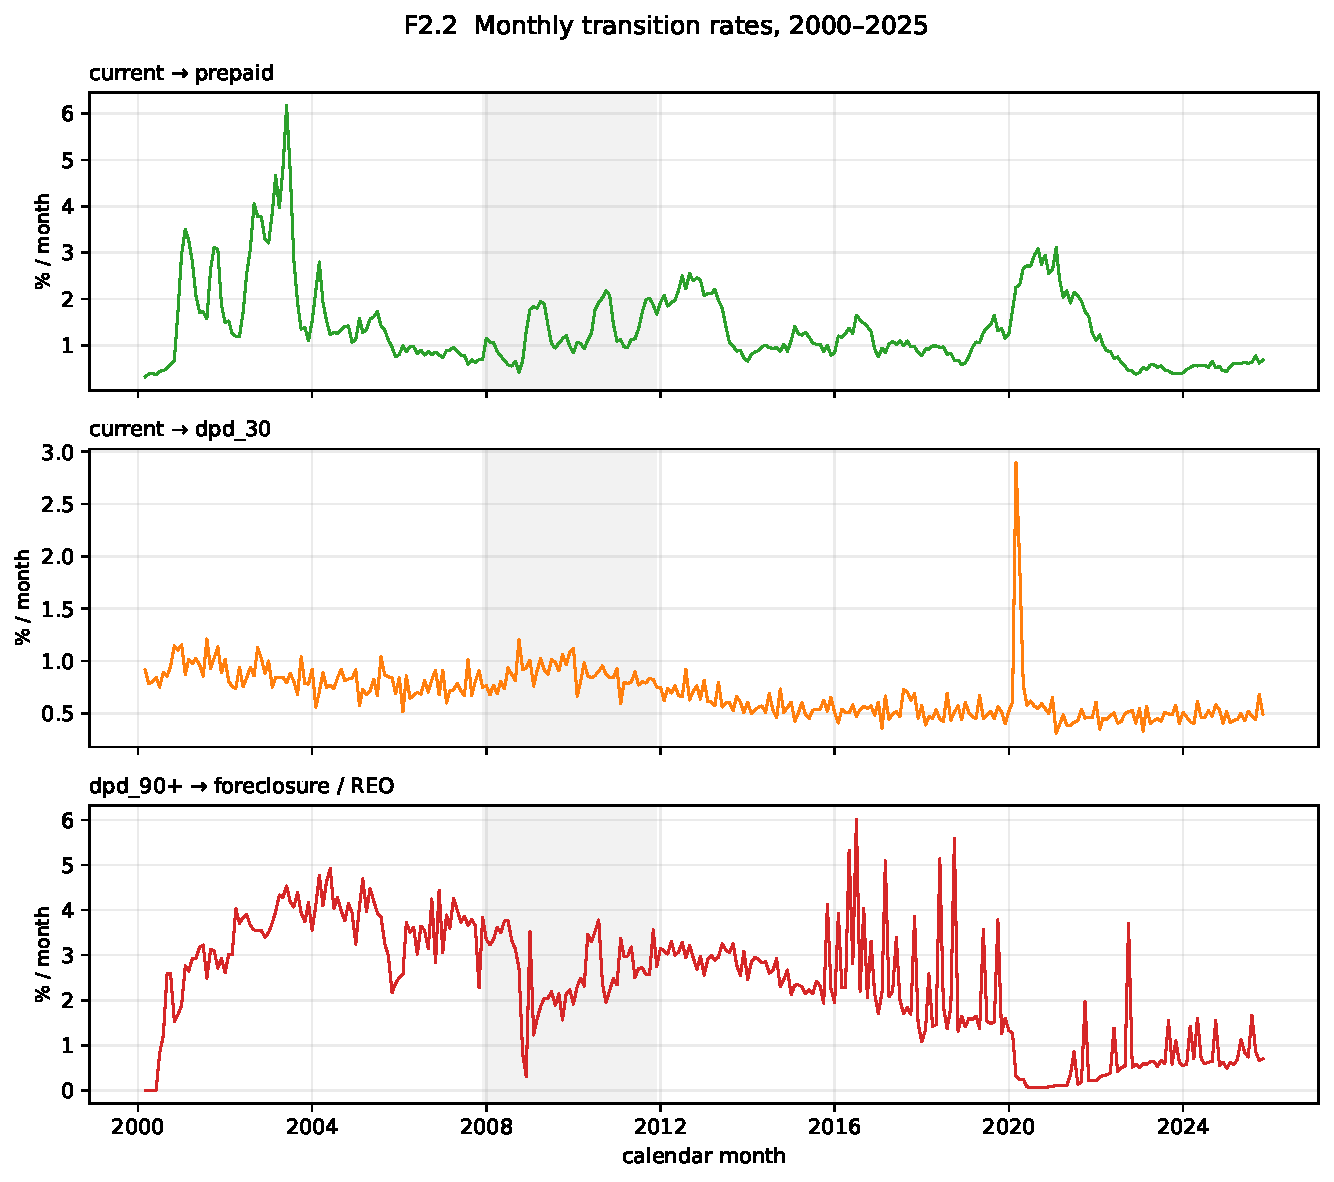
\includegraphics[width=0.9\textwidth]{figs/F2.2_transition_rates.pdf}
\caption[Monthly transition rates out of the Current state]{Monthly
transition rates out of the Current state, 2000--2025: prepayment and
entry into 30\,DPD (left axis), serious-delinquency terminations
(right axis).  Vertical shading marks the 2008--11 crisis and the
2020--21 forbearance episode.}\label{fig:transitionrates}
\end{figure}

\begin{table}[htbp]\centering\small
\caption[Summary statistics of model covariates]{Summary statistics of
the continuous model covariates over the full panel: null rate, mean,
standard deviation, and the min/1st/25th/50th/75th/99th/max
percentiles.}\label{tab:covariate-summary}
\resizebox{\textwidth}{!}{\input{figs/T1.2_covariate_summary.tex}}
\end{table}

% ────────────────────────────────────────────────────────────
\section{Exploratory Evidence: Nonlinearity and Interactions}
\label{sec:data-eda}

Before any model is fitted, the case that nonlinear modelling is
\emph{needed} can be made by counting alone.  The instrument is the
empirical hazard curve: bucket a covariate into equal-population
bins and plot the realised one-month transition rate per bin, with
Wilson 95\% confidence intervals.  Because each curve is a single
out-of-core aggregation over the columnar panel, the entire
programme runs in minutes.

\subsection{Single-covariate nonlinearity}
\label{subsec:data-eda-single}

Three hazard curves carry the argument.
\emph{Prepayment versus loan age}
(Figure~\ref{fig:hazard-age}): the rate rises from $0.27\%$ per month
at origination to a peak of $1.56\%$ at approximately 17 months of
age, then decays to $1.11\%$ by month 52 --- the classic
``seasoning hump,'' strongly non-monotone, with a secondary late-life
rise among long-surviving loans.  \emph{Prepayment versus the
refinancing incentive} (Figure~\ref{fig:hazard-incentive}): the rate
is flat at $0.4$--$0.6\%$ per month while the option is out of the
money, turns up sharply through zero, peaks at $2.71\%$ near
$+1.5$ percentage points of incentive, and falls back to $2.16\%$ by
$+2.7$ --- a roughly sevenfold range containing both an inflection
and a turning point, reproducing the flagship nonlinearity of
\citet{sirignano2021} on this cleaner credit box.
\emph{Delinquency versus credit score}
(Figure~\ref{fig:hazard-fico}): the entry rate into 30\,DPD falls
twenty-four-fold, from $3.06\%$ per month at FICO ${\approx}623$ to
$0.13\%$ at FICO ${\approx}815$, and the decay is convex --- the
slope in the low-score half is roughly $3.7$ times that in the
high-score half.  None of the three shapes is representable by a
linear term.

\begin{figure}[htbp]\centering
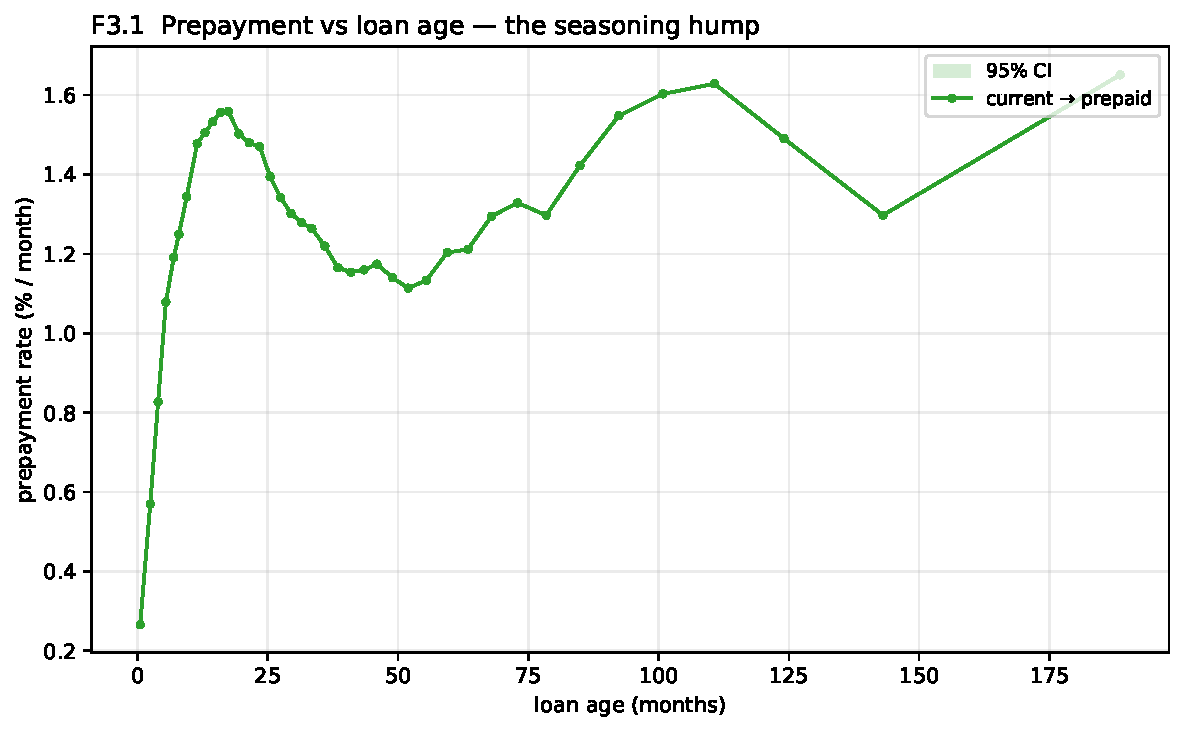
\includegraphics[width=0.8\textwidth]{figs/F3.1_prepay_age.pdf}
\caption[Empirical prepayment hazard by loan age]{Empirical prepayment
hazard by loan age (equal-population buckets, Wilson 95\% intervals):
the seasoning hump.}\label{fig:hazard-age}
\end{figure}

\begin{figure}[htbp]\centering
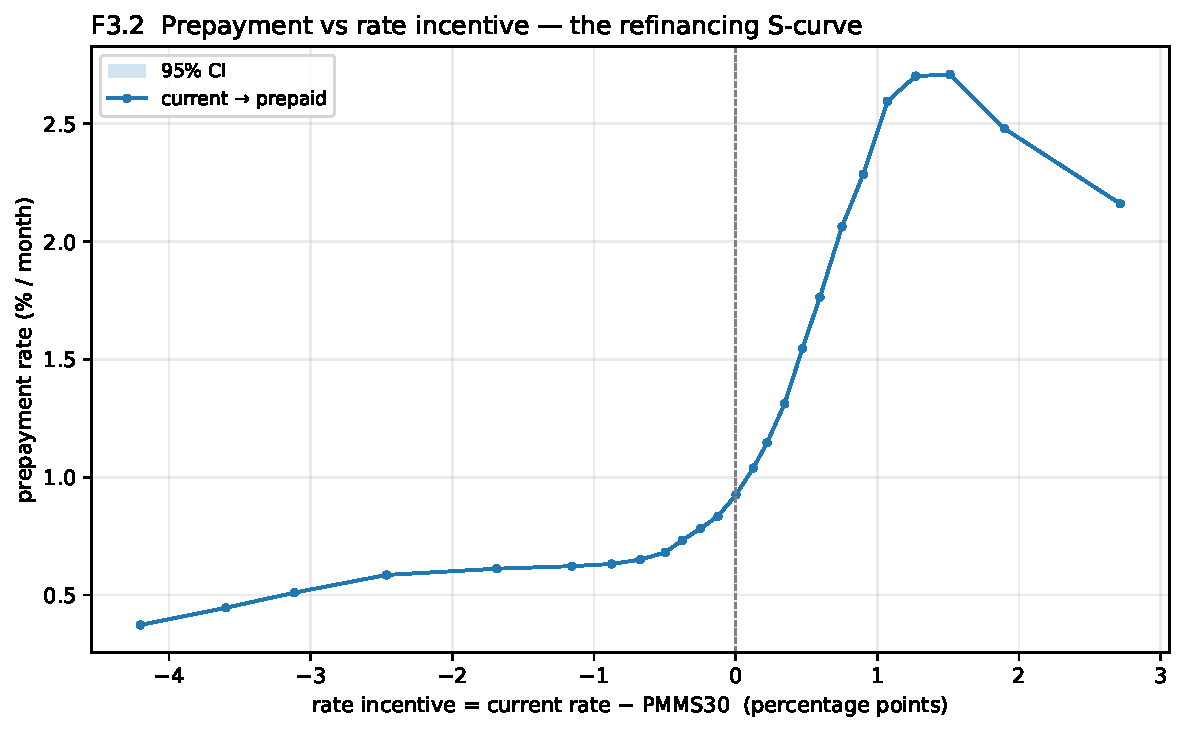
\includegraphics[width=0.8\textwidth]{figs/F3.2_prepay_incentive.pdf}
\caption[Empirical prepayment hazard by refinancing incentive]{Empirical
prepayment hazard by refinancing incentive: the S-curve, with burnout
beyond $+1.5$\,pp.}\label{fig:hazard-incentive}
\end{figure}

\begin{figure}[htbp]\centering
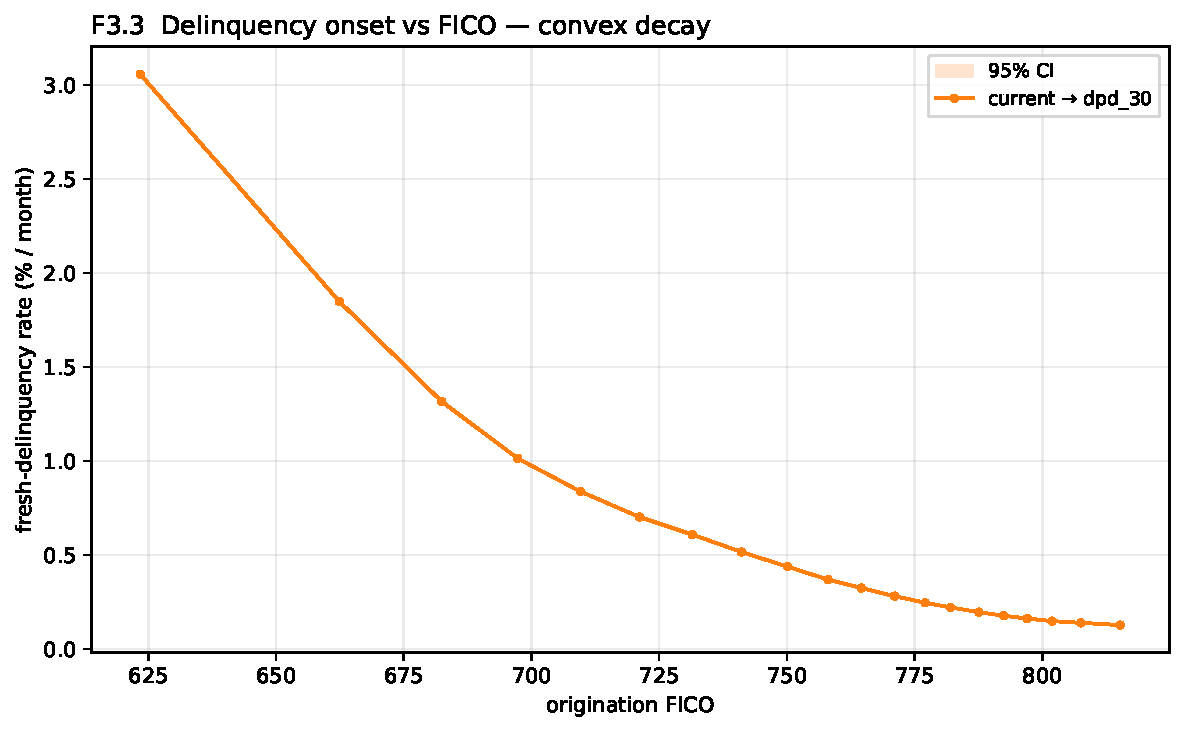
\includegraphics[width=0.8\textwidth]{figs/F3.3_delinq_fico.pdf}
\caption[Empirical 30\,DPD entry hazard by origination credit
score]{Empirical 30\,DPD entry hazard by origination credit score:
convex decay.}\label{fig:hazard-fico}
\end{figure}

\subsection{Interactions: the case against additivity}
\label{subsec:data-eda-interactions}

A linear-\emph{additive} model could in principle be patched with
transformed single-variable terms; interactions are what it cannot
absorb.  On a credit-score~$\times$~LTV grid
(Figure~\ref{fig:interaction-ficoltv}), the monthly rate of entry
into delinquency ranges from $0.11\%$ (best scores, lowest leverage)
to $2.69\%$ (worst scores, highest leverage) --- and decisively, the
\emph{additive} credit-score gradient (worst-minus-best rate) grows
from $1.73$ percentage points at low LTV to $2.48$ at high LTV, a
$43\%$ increase; equivalently, the leverage effect is roughly
$8.5$ times larger for low-score than high-score borrowers.
Additivity forces this gradient to be constant; the violation sits
exactly in the low-score/high-leverage corner that drives credit
losses.  In the prepayment channel
(Figure~\ref{fig:interaction-incfico}), splitting the incentive
S-curve by credit-score tercile shows the in-the-money refinancing
response \emph{rising} with credit quality --- $2.36\%$ per month in
the lowest tercile against $3.01\%$ in the highest --- because
credit-constrained borrowers cannot exercise the option: the
incentive \emph{slope} itself depends on the score.  Finally, holding
loan age fixed at 12--36 months to strip out seasoning, the
delinquency hazard by origination cohort isolates a clean vintage
effect: the 2007 cohort peaks at $1.68\%$ per month against $0.47\%$
for calm cohorts --- a $3.6$-fold premium
(Figure~\ref{fig:vintage}) --- so the origination vintage is a
feature in its own right, not reducible to contemporaneous
covariates.

\begin{figure}[htbp]\centering
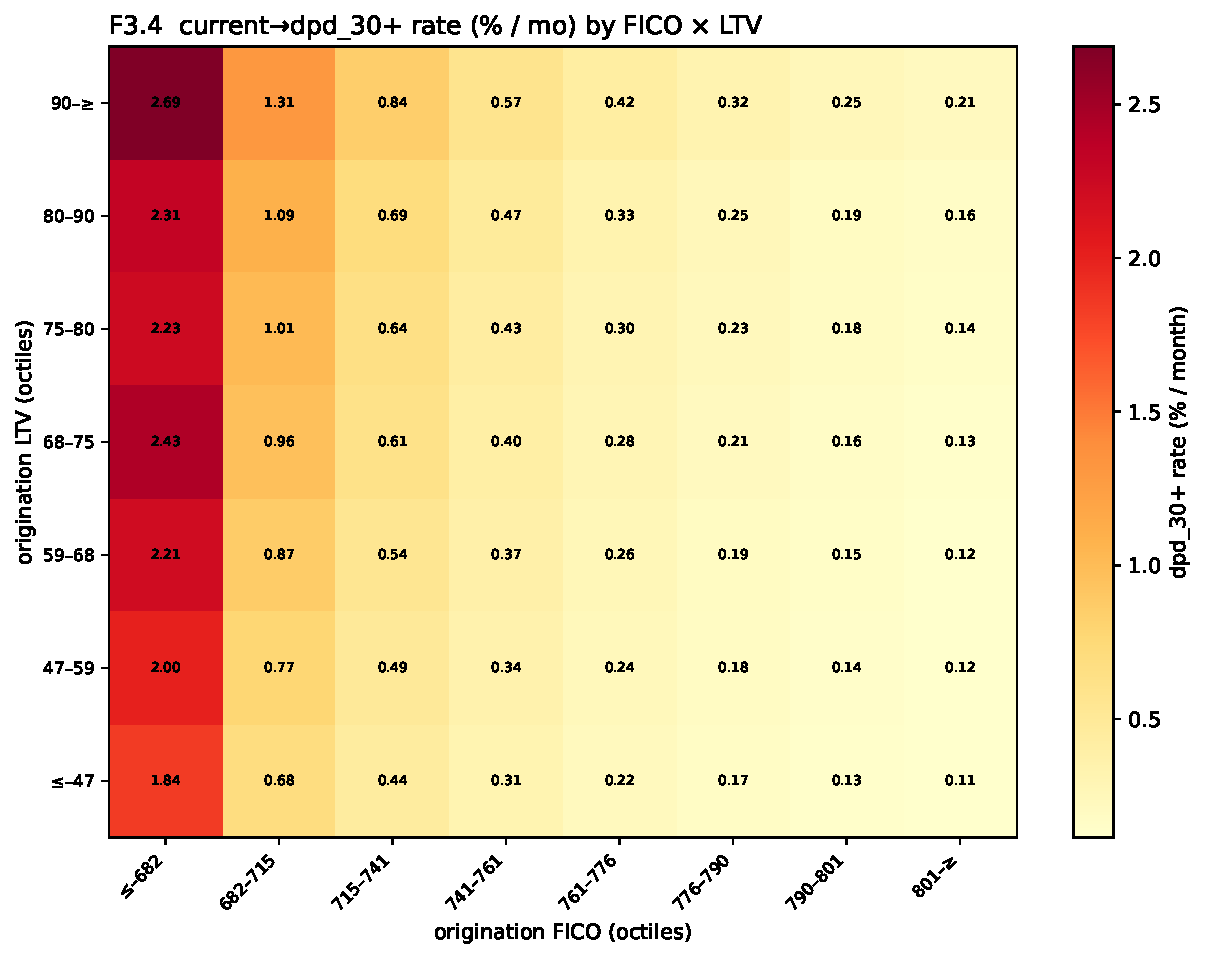
\includegraphics[width=0.78\textwidth]{figs/F3.4_fico_ltv_heatmap.pdf}
\caption[Monthly delinquency-entry rate on a credit-score $\times$ LTV
grid]{Monthly delinquency-entry rate on a credit-score $\times$ LTV grid
(equal-population bands): the additive credit-score gradient grows with
leverage --- additivity is misspecified.}\label{fig:interaction-ficoltv}
\end{figure}

\begin{figure}[htbp]\centering
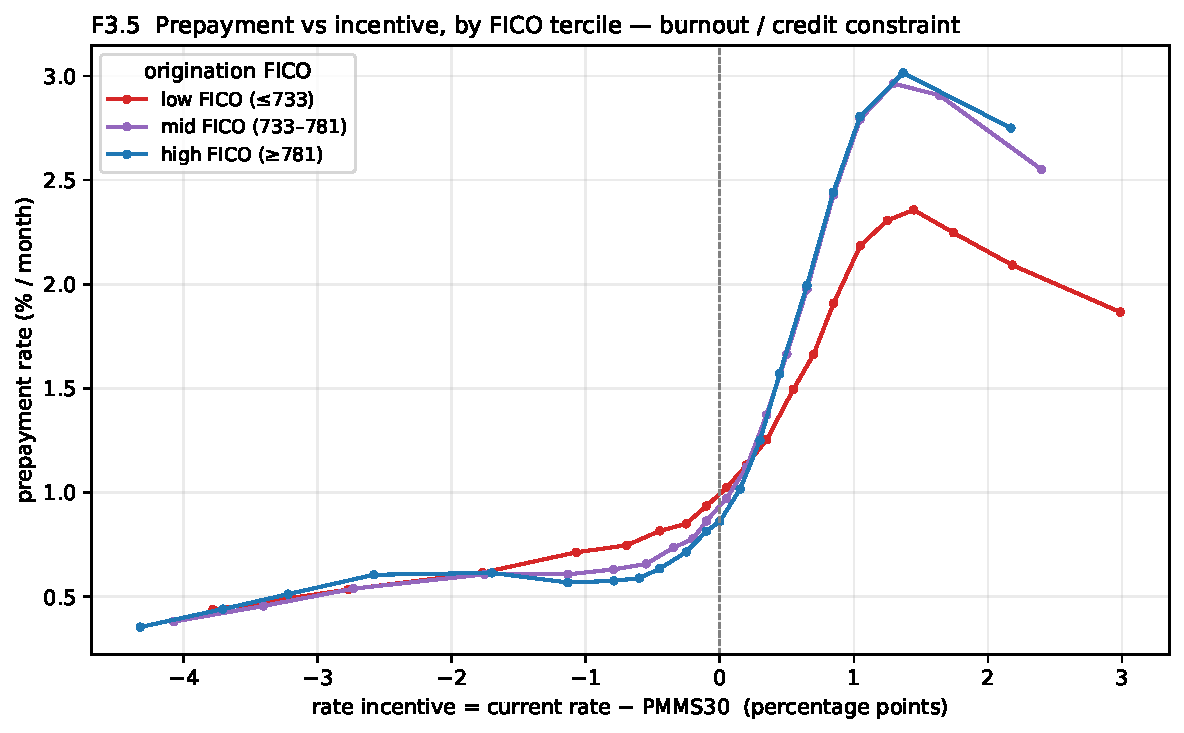
\includegraphics[width=0.8\textwidth]{figs/F3.5_incentive_fico.pdf}
\caption[The incentive S-curve by credit-score tercile]{The incentive
S-curve by credit-score tercile: the refinancing response to an
in-the-money option rises with credit
quality.}\label{fig:interaction-incfico}
\end{figure}

\begin{figure}[htbp]\centering
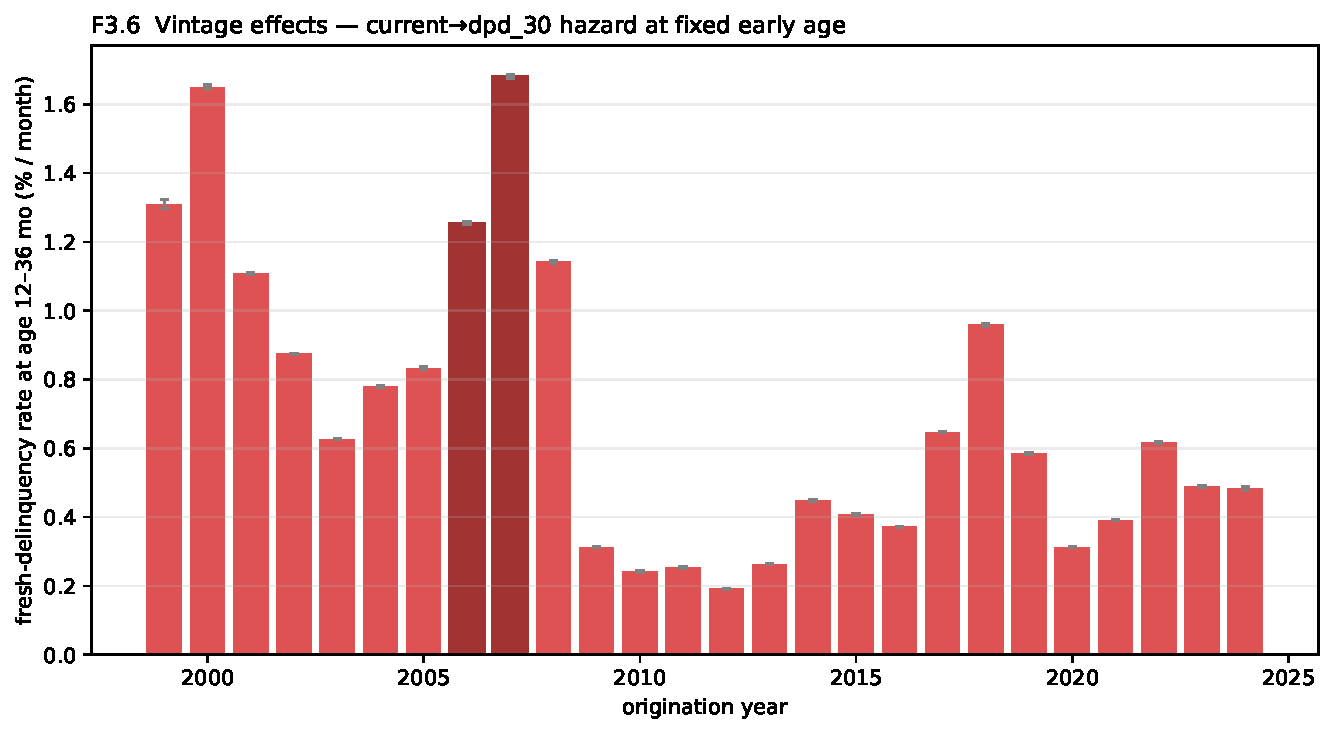
\includegraphics[width=0.8\textwidth]{figs/F3.6_vintage.pdf}
\caption[Delinquency hazard by origination cohort at fixed loan
age]{Delinquency hazard by origination cohort at fixed loan age
(12--36 months): the 2006--08 bubble vintages.}\label{fig:vintage}
\end{figure}

Taken together, the evidence points one way: monthly transition risk
depends on the covariates nonlinearly (the seasoning hump, the
incentive S-curve, convex credit-score decay) and interactively
(score$\times$leverage, incentive$\times$score, vintage).  A
linear-additive model should therefore underfit --- most severely on
prepayment, the channel combining the sharpest single-variable
nonlinearity with a first-order interaction --- and
Chapter~\ref{chap:results} tests precisely this.

% ────────────────────────────────────────────────────────────
\section{Comparison to Sirignano et al.\ (2021)}
\label{sec:data-comparison}

The dataset employed in the present study differs in several important
respects from the proprietary CoreLogic dataset used by
\citet{sirignano2021}, and these differences bear on the
interpretation of the results.

\citet{sirignano2021} draw on records for approximately 120 million
mortgages --- both prime and subprime --- originated across the United
States between January 1995 and June 2014, yielding approximately 3.5
billion loan-month observations.  The CoreLogic data encompass the
full spectrum of mortgage products, including fixed-rate,
adjustable-rate, hybrid, balloon, and interest-only loans, as well as
government-insured instruments.  Macro-economic covariates ---
zip-code-level house price indices from Zillow, county-level
unemployment rates from the Bureau of Labor Statistics, and the
Freddie Mac PMMS series --- are merged at the loan-month level within
the CoreLogic database.  The dataset is proprietary and cannot be
reproduced by independent researchers.

The Fannie Mae primary dataset, by contrast, is limited to
conventional fixed-rate fully-amortising loans and excludes both
subprime and government-insured products.  Macro-economic covariates
must be sourced and joined externally, as described in
Section~\ref{subsec:data-external}.  These differences have two
principal consequences.  First, the estimation sample is more
homogeneous in product mix; the nonlinear prepayment dynamics
associated with adjustable-rate burnout and subprime option exercise
--- prominent in \citeauthor{sirignano2021} --- are absent.  Second,
the absence of a subprime segment limits the range of credit-risk
outcomes observed; \citet{sirignano2021} report a median FICO score
of 630 for their subprime sub-sample against 730 for the prime
sub-sample, whereas the Fannie Mae population is concentrated at the
higher end of this credit-quality spectrum.

These limitations notwithstanding, the Fannie Mae dataset provides a
fully reproducible basis for the analysis.  The core methodological
contribution of \citet{sirignano2021} --- applying deep learning to a
multinomial competing-risks model of monthly loan-state transitions
--- transfers completely to the Fannie Mae panel.  The architecture,
estimation procedure, and evaluation framework described in subsequent
chapters are direct adaptations of that approach.  Table~\ref{tab:data-comparison}
summarises the key differences.

\begin{table}[htbp]
  \centering
  \small
  \begin{tabularx}{\textwidth}{@{} l X X @{}}
    \toprule
    \textbf{Dimension}
      & \textbf{Sirignano et al.\ (2021)}
      & \textbf{Present study} \\
    \midrule
    Data source
      & CoreLogic (proprietary)
      & Fannie Mae SFLP (public) \\[3pt]
    Total loans
      & ${\sim}120$ million
      & 57.6 million \\[3pt]
    Loan-month observations
      & ${\sim}3.5$ billion
      & 3.31 billion \\[3pt]
    Origination window
      & 1995--2014
      & 1999--2025 (full vintage set, reporting to 2025-12) \\[3pt]
    Products covered
      & Fixed, ARM, hybrid, balloon, IO
      & Fixed-rate, fully amortising only \\[3pt]
    Credit segments
      & Prime and subprime
      & Conventional (predominantly prime) \\[3pt]
    Macro covariates
      & Embedded (Zillow, BLS, PMMS)
      & External join required (FHFA HPI, PMMS) \\[3pt]
    Geographic detail
      & Full 5-digit zip code
      & 3-digit truncated zip; MSA \\[3pt]
    States modelled
      & Seven
      & Seven (identical mapping) \\[3pt]
    Reproducibility
      & Not publicly reproducible
      & Fully reproducible \\
    \bottomrule
  \end{tabularx}
  \caption[Comparison of the Fannie Mae SFLP dataset and the
  CoreLogic dataset used by Sirignano et al.\ (2021)]%
  {\textit{Comparison of the Fannie Mae SFLP primary dataset and the
  CoreLogic dataset used by \citet{sirignano2021}.}  CoreLogic counts
  are approximate as reported by the authors; Fannie Mae counts are
  measured on the assembled panel (Section~\ref{sec:data-summary}).}
  \label{tab:data-comparison}
\end{table}

%  to main.tex (after chapter2, before conclusions).
%
%  Required packages (add to the preamble of main.tex):
%      \usepackage{booktabs}
%      \usepackage{tabularx}
%      \usepackage{multirow}
%      \usepackage{natbib}   % or your preferred bib style
% ============================================================

\chapter{Data}
\label{chap:data}

% ────────────────────────────────────────────────────────────
\section{Data Source}
\label{sec:data-source}

This study employs the Fannie Mae Single-Family Loan Performance
(SFLP) dataset, a publicly available research dataset maintained by
the Federal National Mortgage Association (Fannie Mae) and updated on
a quarterly basis.  The dataset was originally released in April 2013
and contains origination and monthly performance records for a subset
of single-family conventional mortgage loans acquired by Fannie Mae
since January 2000.  New loan acquisitions and performance data are
added with an approximate four-month lag following the end of each
calendar quarter \citep{fanniemae2024}.

The data are organised as a \emph{loan-month panel}: each observation
corresponds to a single mortgage loan in a single monthly reporting
period, beginning at the month of acquisition and continuing until the
loan terminates through full prepayment, foreclosure, Real Estate
Owned (REO) disposition, or contractual maturity, or until the data
cut-off date.  This longitudinal structure is well-suited to the
competing-risks framing of \citet{sirignano2021}, which the present
study adapts to the Fannie Mae data.

Raw files are distributed as pipe-delimited CSV without a header row,
organised by acquisition quarter and identified by the convention
\texttt{YYYYQn.csv}.  Column identities are positional, fully
specified in the Fannie Mae Single-Family Loan Performance Data File
Layout and Glossary.  Each row contains 113 fields encoding static
origination attributes, dynamic monthly performance measures, and
post-termination expense and proceeds data.  The estimation sample
employed in this study is the \emph{complete} vintage set from a
single quarterly release: 104 acquisition-quarter files covering
cohorts from 2000Q1 onwards, with monthly reporting periods from
January 2000 through December 2025.  The assembled panel comprises
\textbf{3{,}312{,}456{,}883 loan-month observations across
57{,}562{,}668 loans} --- performance histories spanning four
interest-rate cycles, the 2008--11 foreclosure crisis, the COVID-era
forbearance episode, and the 2022--23 rate shock.

\subsection{From raw files to the estimation panel}
\label{subsec:data-pipeline}

Three distinct concepts in this dataset are colloquially called a
``quarter,'' and distinguishing them prevents the most common
assembly errors.  The \emph{acquisition vintage} identifies a file:
each \texttt{YYYYQn.csv} contains the loans Fannie Mae acquired in
that quarter, carrying their entire subsequent monthly history, and a
loan appears in exactly one file --- so concatenating all files
assembles the full sample with no duplication.  The \emph{monthly
reporting period} identifies a row, and this time dimension --- not
redundancy --- is why the dataset is large.  The \emph{release}
identifies the download: Fannie Mae republishes the entire dataset
quarterly with extended histories, so all files must come from one
release lest vintages carry inconsistent right-censoring dates; an
ingestion audit verifies a uniform cut-off across all 104 files.

Because no single file fits in memory ($\sim$800\,GB of raw CSV in
total), a six-stage pipeline converts the files into a compressed,
columnar store queried out of core: an integrity audit, streaming
conversion, type and sentinel cleaning, construction of the
transition panel with the outcome variable of
Section~\ref{sec:data-outcome}, sampling utilities, and a
reconciliation step that verifies row counts against the raw files.
Columnar storage means a query touching six of the 113 fields reads
roughly five per cent of the bytes, which is what makes the
full-panel descriptive statistics and exploratory analysis of
Sections~\ref{sec:data-summary} and~\ref{sec:data-eda}
computationally cheap.

% ────────────────────────────────────────────────────────────
\section{Population and Eligibility}
\label{sec:data-population}

The primary dataset is not a census of all loans in Fannie Mae's
guarantee book; it is a curated research sample subject to documented
eligibility and exclusion criteria \citep{fanniemae2024}.  The
population is restricted to fixed-rate, fully amortising,
full-documentation single-family conventional mortgage loans with
original terms of at least five years and less than 35 years,
originated on or after 1 January 1999 and acquired by Fannie Mae on
or after 1 January 2000.

A number of product types are explicitly excluded.  Adjustable-rate
mortgages, interest-only loans, balloon-amortisation mortgages, and
loans carrying prepayment penalties are absent from the dataset.
Also excluded are loans with original loan-to-value (LTV) ratios
exceeding 97 per cent, Alt-A and other reduced-documentation
products, government-insured loans (FHA and VA), loans subject to
long-term standby commitments or third-party risk-sharing
arrangements other than primary mortgage insurance, and loans
acquired on a negotiated bulk basis.  Loans with non-standard payment
due dates and loans that liquidated in the same month as acquisition
are similarly excluded.  Fannie Mae's Home Affordable Refinance
Program (HARP) loans are likewise absent from the primary dataset;
when a loan in the primary dataset was subsequently refinanced through
HARP, its termination is recorded as a standard prepayment, and its
post-refinance performance is not tracked here.  This is discussed
further in Section~\ref{sec:data-outcome}.

These restrictions yield a sample of conventionally underwritten
fixed-rate mortgages broadly representative of the agency conventional
loan market under post-crisis underwriting standards.  The exclusion
of adjustable-rate and interest-only products limits the range of
prepayment incentive dynamics captured relative to the full-spectrum
dataset used by \citet{sirignano2021}; this is discussed in
Section~\ref{sec:data-comparison}.  Table~\ref{tab:eligibility}
summarises the principal eligibility criteria and exclusions.

\begin{table}[htbp]
  \centering
  \small
  \begin{tabularx}{\textwidth}{@{} l X @{}}
    \toprule
    \textbf{Criterion} & \textbf{Requirement / Exclusion} \\
    \midrule
    Origination date      & On or after 1 January 1999 \\[2pt]
    Acquisition date      & On or after 1 January 2000 \\[2pt]
    Product type          & Fixed-rate, fully amortising only \\[2pt]
    Loan term             & $5 \leq \mathrm{term} < 35$ years at origination \\[2pt]
    Documentation         & Full documentation only \\[2pt]
    LTV at origination    & $\leq 97\%$ \\[4pt]
    \emph{Excluded: product}      & ARM, interest-only, balloon,
                                    prepayment-penalty loans \\[2pt]
    \emph{Excluded: credit class} & Alt-A, reduced-documentation,
                                    streamlined processing \\[2pt]
    \emph{Excluded: guarantee}    & Government-insured (FHA, VA) loans \\[2pt]
    \emph{Excluded: structure}    & Long-term standby commitments;
                                    bulk acquisitions; lender-recourse
                                    loans (except primary MI) \\[2pt]
    \emph{Excluded: programme}    & HARP and Refi Plus loans \\[2pt]
    \emph{Excluded: payment}      & Bi-weekly and non-first-of-month
                                    due dates \\[2pt]
    \emph{Excluded: timing}       & Loans liquidated in month of
                                    acquisition \\
    \bottomrule
  \end{tabularx}
  \caption[Eligibility criteria for the Fannie Mae SFLP primary dataset]%
  {\textit{Eligibility criteria for the Fannie Mae SFLP primary
  dataset.}  Source: Fannie Mae Single-Family Loan Performance
  Dataset FAQs \citep{fanniemae2024}.}
  \label{tab:eligibility}
\end{table}

% ────────────────────────────────────────────────────────────
\section{Variables}
\label{sec:data-variables}

The 113 fields in each monthly observation can be organised into three
functional groups: static origination attributes, dynamic monthly
performance attributes, and post-termination resolution data.  The
model uses a subset of these fields as covariates.  Two fields --- the
Current Loan Delinquency Status and the Zero Balance Code --- serve as
the primary inputs from which the outcome variable is constructed.

% ────────────────────────────────
\subsection{Origination Attributes}
\label{subsec:data-origination}

Static origination attributes are recorded at loan delivery and do
not change over the life of the loan absent a modification.  The
borrower's FICO credit score at origination is available for both the
primary borrower and, where applicable, a co-borrower; prior to the
January 2015 dataset release only the lower of the two scores was
disclosed, and a missingness indicator is constructed accordingly.
Continuous origination covariates include the original
debt-to-income (DTI) ratio, original LTV ratio, original combined LTV
(CLTV, which incorporates subordinate liens), original unpaid
principal balance (UPB), original interest rate, and original loan
term in months.  Categorical origination attributes include the
acquisition channel (retail, broker, or correspondent), loan purpose
(purchase, rate-term refinance, or cash-out refinance), property type,
occupancy status (primary residence, second home, or investment
property), property state, Metropolitan Statistical Area (MSA), and
three-digit truncated zip code.  The truncation of the zip code
reflects borrower privacy considerations; full zip codes are not
disclosed in the dataset \citep{fanniemae2024}.

% ────────────────────────────────
\subsection{Dynamic Performance Attributes}
\label{subsec:data-performance}

Dynamic performance attributes are updated in each monthly reporting
period.  The current actual unpaid principal balance reflects the
outstanding loan balance at each point in time.  Loan age, measured
in months from the first payment date, and the remaining months to
legal maturity are derived from the contractual amortisation schedule.
The current interest rate reflects the applicable note rate, updated
when a modification changes the loan terms.

Two dynamic fields jointly determine the outcome variable.  The
\textbf{Current Loan Delinquency Status} reports the number of missed
monthly payments as a two-character code: \texttt{00} denotes a
current loan; \texttt{01}, \texttt{02}, and codes \texttt{03} and
above denote 30-, 60-, and 90-or-more-day delinquencies respectively;
and \texttt{XX} denotes an unavailable status.  The \textbf{Zero
Balance Code} is populated exclusively in the terminal monthly
observation and classifies the manner of loan termination into nine
categories, distinguishing between voluntary prepayments, third-party
foreclosure sales, short sales, repurchases, REO dispositions, note
sales, and non-credit removals.  (The dataset also carries a 24-month
payment-history string; it is not used as a model input here, since
the current state and loan-level covariates already summarise the
information the transition model conditions on.)

% ────────────────────────────────
\subsection{Externally Sourced Covariates}
\label{subsec:data-external}

A small, fixed set of external macroeconomic series is joined to the
loan-level panel at feature-construction time (the stored panel
itself is never rewritten); Table~\ref{tab:macrovars} summarises the
sources.  The Freddie Mac Primary Mortgage Market Survey (PMMS)
weekly fixed-rate series, aggregated to calendar-month means, supplies
the prevailing market mortgage rate from which the \emph{rate
incentive} of Equation~\eqref{eq:incentive} is computed --- the
refinancing option value, the primary driver of prepayment behaviour
in the empirical mortgage literature
\citep{schwartz1989,sirignano2021}.  Unemployment rates enter at both
national (Bureau of Labor Statistics) and state level, the latter
because the cross-sectional dispersion in labour-market conditions
(Nevada versus Texas in 2009) is precisely the variation a national
series cannot supply.  House prices enter through the Freddie Mac
House Price Index at national and state level, from which the
mark-to-market loan-to-value ratio of Equation~\eqref{eq:mtmltv} ---
the principal determinant of the default option value
\citep{deng2000} --- and the trailing twelve-month house-price change
are constructed.  The ten-year Treasury yield completes the set.

Each series is joined with a \emph{publication lag} reflecting when
the value was actually observable: rates are published in real time
(no lag), month-$t$ unemployment is released early in month $t{+}1$
(one-month lag), and the house-price index roughly two months after
the reference month (two-month lag).  Final-revision series are used
rather than real-time vintages --- a stated limitation, standard for
historical studies.  Where a state-level value is unavailable
(territories; series start dates) the national value substitutes,
with an indicator flag carried as a model feature.

\begin{table}[htbp]
  \centering
  \small
  \begin{tabularx}{\textwidth}{@{} l l l l c @{}}
    \toprule
    \textbf{Variable} & \textbf{Source} & \textbf{Geography}
      & \textbf{Monthly value} & \textbf{Lag} \\
    \midrule
    30-yr mortgage rate & Freddie Mac PMMS & national & month mean & 0\,m \\
    10-yr Treasury yield & FRED \texttt{DGS10} & national & month mean & 0\,m \\
    Unemployment rate & BLS (via FRED) & national + state & as published & 1\,m \\
    House-price index & Freddie Mac FMHPI & national + state & as published & 2\,m \\
    \bottomrule
  \end{tabularx}
  \caption[External macroeconomic covariates and join conventions]%
  {\textit{External macroeconomic covariates and join conventions.}
  A loan-month at calendar month $t$ is joined to the macro value of
  month $t-\ell$, where $\ell$ is the publication lag.  Seasonally
  adjusted versions are used throughout.}
  \label{tab:macrovars}
\end{table}

As a check on the incentive variable, a market-rate proxy derived
from the panel itself --- the average note rate of loans originated
in each calendar month --- tracks the PMMS series with correlation
$0.991$, root-mean-square deviation $0.198$ percentage points, and
mean absolute deviation $0.147$ percentage points, with a mean gap of
essentially zero.  The PMMS-based incentive is the primary feature;
the panel-derived proxy is retained as a robustness alternative,
demonstrating that the incentive variable is not an artefact of one
data source.

% ────────────────────────────────────────────────────────────
\section{Outcome Variable}
\label{sec:data-outcome}

Following \citet{sirignano2021}, the outcome variable is a categorical
measure of mortgage state in month $t+1$, conditional on the loan's
state and covariate vector in month $t$.  Seven mutually exclusive
states are defined: \emph{Current}, \emph{30 Days Past Due}
(30\,DPD), \emph{60 Days Past Due} (60\,DPD), \emph{90+ Days Past
Due} (90+\,DPD), \emph{Foreclosure}, \emph{Real Estate Owned} (REO),
and \emph{Prepaid}.

State assignment for each loan-month observation follows a
deterministic hierarchy.  When the Zero Balance Code is present ---
indicating the terminal observation for the loan --- the termination
type is mapped to the Foreclosure, REO, or Prepaid absorbing state as
shown in Table~\ref{tab:state-mapping}.  When the Zero Balance Code is
absent, the delinquency status field governs: codes \texttt{00}
through \texttt{03} and above map to Current, 30\,DPD, 60\,DPD, and
90+\,DPD respectively, while \texttt{XX} is treated as missing.  The
state in month $t+1$ is obtained by a window lead over the reporting
period dimension, partitioned by loan identifier.  Loans whose final
observation falls at or before the data cut-off without a recorded
termination event receive a censored indicator and are excluded from
the labelled target.

Regarding HARP loans: as noted in Section~\ref{sec:data-population},
any loan in the primary dataset that was refinanced through the
HARP programme terminates with a Zero Balance Code of \texttt{01}
(prepaid) at the moment of refinancing and is therefore treated as a
standard prepayment in the outcome variable.  This approximation is
defensible given that the loan is extinguished from Fannie Mae's
credit exposure in either case, though it may marginally overstate
the rate-incentive sensitivity of the prepayment hazard during the
period of peak HARP activity (approximately 2009--2013).

\begin{table}[htbp]
  \centering
  \small
  \begin{tabularx}{\textwidth}{@{} l l l X @{}}
    \toprule
    \textbf{State} & \textbf{Source field} & \textbf{Condition}
      & \textbf{Economic interpretation} \\
    \midrule
    Current
      & Delinquency Status & \texttt{= 00}
      & Borrower is contractually current on all payments. \\[3pt]
    30\,DPD
      & Delinquency Status & \texttt{= 01}
      & One missed monthly payment. \\[3pt]
    60\,DPD
      & Delinquency Status & \texttt{= 02}
      & Two consecutive missed monthly payments. \\[3pt]
    90+\,DPD
      & Delinquency Status & \texttt{$\geq$ 03}
      & Three or more missed payments; serious delinquency. \\[3pt]
    Foreclosure
      & Zero Balance Code  & \texttt{02, 03, 15,}
      & Credit-loss termination: third-party sale, short sale, \\
      &                    & \texttt{97, 98}
      & note sale, or credit-event repurchase. \\[3pt]
    REO
      & Zero Balance Code  & \texttt{= 09}
      & Fannie Mae acquires ownership of the property. \\[3pt]
    Prepaid
      & Zero Balance Code  & \texttt{01, 06, 16,}
      & Full payoff, contractual maturity, repurchase, \\
      &                    & \texttt{96}
      & or non-credit removal (including HARP exits). \\
    \bottomrule
  \end{tabularx}
  \caption[Mapping of Fannie Mae data fields to the seven-state
  outcome variable]%
  {\textit{Mapping of Fannie Mae data fields to the seven-state
  outcome variable.}  The Zero Balance Code is populated only in the
  terminal monthly observation; the Delinquency Status governs state
  assignment in all non-terminal periods.}
  \label{tab:state-mapping}
\end{table}

One structural feature of this dataset deserves emphasis: because the
Foreclosure, REO, and Prepaid states are derived from the Zero
Balance Code --- populated only in a loan's final observation ---
these three states are \emph{absorbing}.  There is no ongoing ``in
foreclosure'' monthly status as in the CoreLogic data of
\citet{sirignano2021}, where loans in formal foreclosure are observed
month by month and occasionally return to performing status.  The
origin set here therefore comprises the four live states (Current
through 90+\,DPD) while destinations span all seven: the transition
matrix is $4\times 7$ rather than $7\times 7$
(Section~\ref{sec:meth-model}).  Within the live states the data are
rich in both directions --- delinquency deepens at most one bucket
per month, but cures can jump multiple buckets, and a meaningful
fraction of seriously delinquent loans return to current.  The
seven-state formulation captures this in a way that a binary
default-versus-prepayment classification would obscure, and the
empirical monthly transition matrix derived from each training window
serves as the floor benchmark for the model comparison
(Section~\ref{subsec:meth-empirical}).

% ────────────────────────────────────────────────────────────
\section{Panel Composition and Summary Statistics}
\label{sec:data-summary}

The assembled panel comprises 3{,}312{,}456{,}883 loan-month
observations across 57{,}562{,}668 loans in 104 acquisition-vintage
partitions, with reporting months from January 2000 through December
2025.  Table~\ref{tab:stateshares} reports the distribution of
loan-months across the seven states.  Two features dominate.  First,
extreme class imbalance: the Current state accounts for $96.28\%$ of
all loan-months, while the credit-event terminals occur at roughly
one in ten thousand observations --- the empirical fact behind both
the importance-weighted thinning of training data
(Section~\ref{sec:meth-design}) and the Laplace smoothing of the
empirical benchmark (Section~\ref{subsec:meth-empirical}).  Second,
the rare states are nonetheless abundantly populated in absolute
terms (REO alone contributes roughly half a million loan-months),
which is what permits stable estimation of rare-transition
probabilities at this scale.

\begin{table}[htbp]
  \centering
  \small
  \begin{tabular}{l r @{\qquad\qquad} l r}
    \toprule
    \textbf{State} & \textbf{Share} & \textbf{State} & \textbf{Share} \\
    \midrule
    Current  & 96.28\,\% & 60\,DPD     & 0.31\,\%   \\
    Prepaid  & 1.25\,\%  & REO         & 0.014\,\%  \\
    30\,DPD  & 1.15\,\%  & Foreclosure & 0.0067\,\% \\
    90+\,DPD & 0.98\,\%  &             &            \\
    \bottomrule
  \end{tabular}
  \caption[Distribution of loan-months across the seven states]%
  {\textit{Distribution of loan-months across the seven states},
  full panel, 2000--2025 (3.31 billion loan-months).}
  \label{tab:stateshares}
\end{table}

Pooled over time, the monthly transition rates out of Current are
$1.27\%$ to Prepaid and $0.64\%$ to 30\,DPD.  The pooling, however,
hides the economics: Figure~\ref{fig:transitionrates} plots the
monthly series over 2000--2025, displaying the 2003 and 2020--21
refinancing waves in the prepayment rate, the 2008--11 default wave
in the delinquency rates, and the sharp 2022--23 collapse in
prepayments as market rates rose.  These regime shifts --- rather
than any single structural break --- are the empirical justification
for the rolling backtest design of Section~\ref{sec:meth-design}.
During 2020--21 the delinquency-status codes additionally reflect
COVID-era forbearance, which manifests as unusual persistence in
delinquency states followed by elevated cure rates; no special
treatment is applied, but results involving those years are read with
this in mind.

\begin{figure}[htbp]\centering
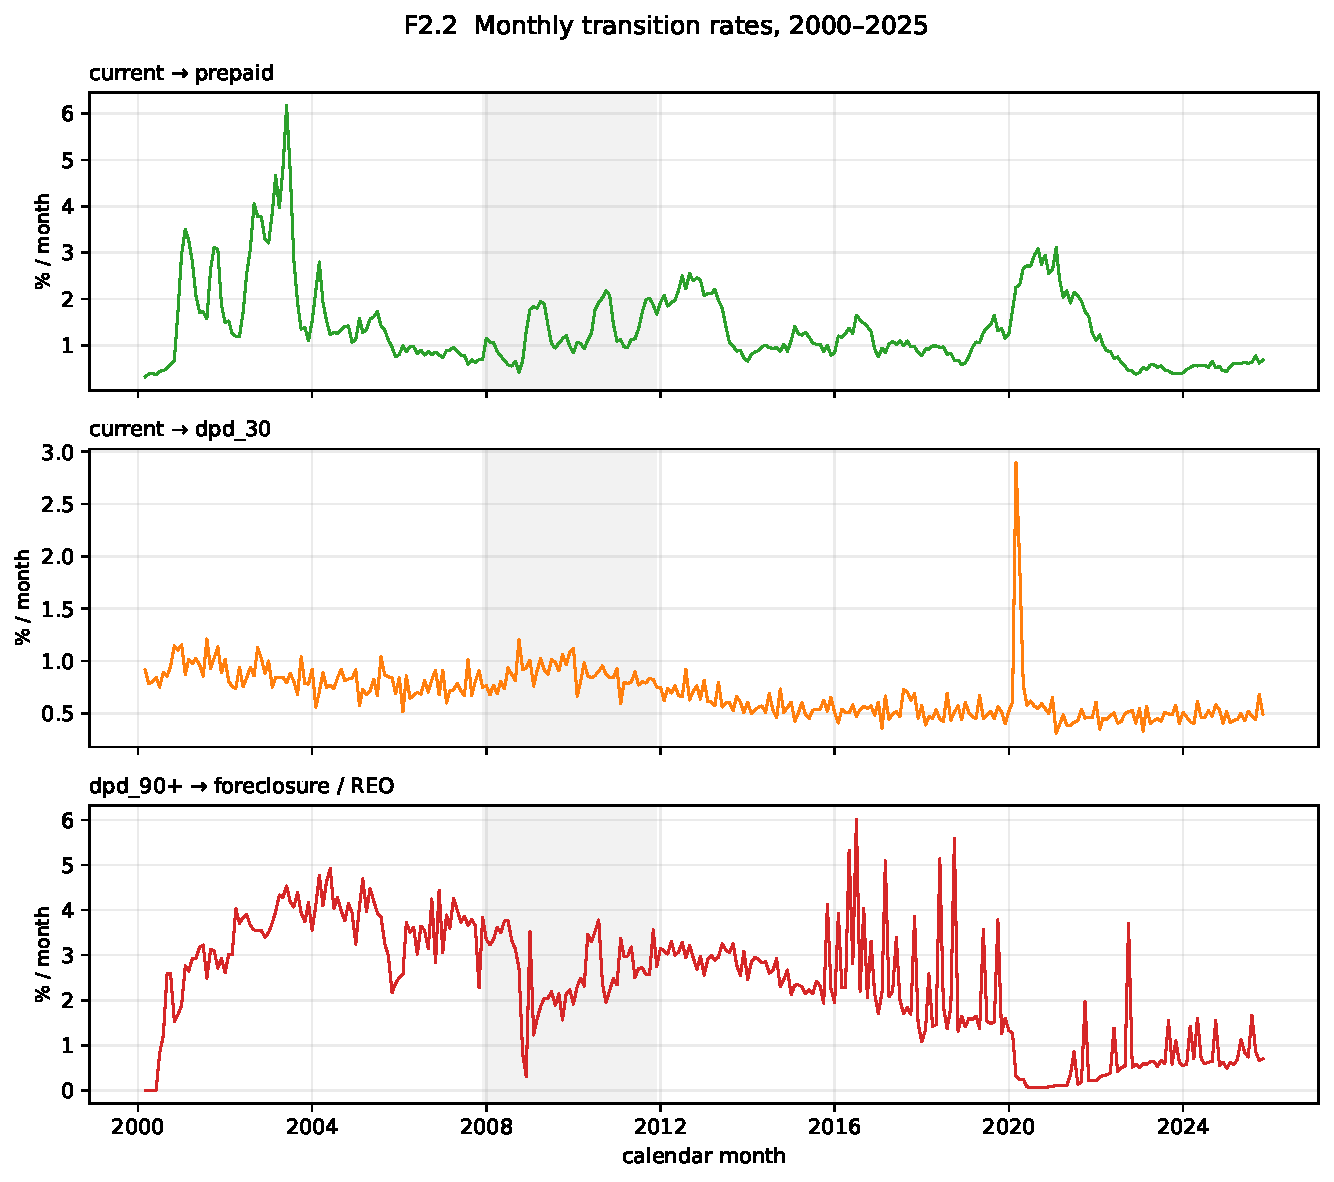
\includegraphics[width=0.9\textwidth]{figs/F2.2_transition_rates.pdf}
\caption[Monthly transition rates out of the Current state]{Monthly
transition rates out of the Current state, 2000--2025: prepayment and
entry into 30\,DPD (left axis), serious-delinquency terminations
(right axis).  Vertical shading marks the 2008--11 crisis and the
2020--21 forbearance episode.}\label{fig:transitionrates}
\end{figure}

\begin{table}[htbp]\centering\small
\caption[Summary statistics of model covariates]{Summary statistics of
the continuous model covariates over the full panel: null rate, mean,
standard deviation, and the min/1st/25th/50th/75th/99th/max
percentiles.}\label{tab:covariate-summary}
\resizebox{\textwidth}{!}{% Source: outputs/tables/eda/T1.2_covariate_summary_continuous.tex (full-panel
% Stage-6 QA). Tabular-only; wrap in \resizebox in chapter3.tex. Caption+label there.
\begin{tabular}{lrrrrrrrrrrl}
\toprule
column & null\_rate & mean & std & min & p01 & p25 & median & p75 & p99 & max & log\_flagged \\
\midrule
Original Interest Rate & 0 & 4.71882 & 1.32648 & 1.5 & 2.36602 & 3.62711 & 4.62688 & 5.75 & 7.85794 & 16.5 & False \\
Current Interest Rate & 0.012707 & 4.68763 & 1.32523 & 0 & 2.28982 & 3.625 & 4.60188 & 5.75 & 7.83746 & 13.5 & False \\
Original UPB & 0 & 199755 & 121639 & 1000 & 38809.4 & 109817 & 170562 & 262260 & 596156 & 2.326e+06 & True \\
Current Actual UPB & 0 & 159715 & 124113 & 0 & 0 & 71875.9 & 134287 & 224204 & 564970 & 2.86e+06 & True \\
Original Loan Term & 0 & 306.643 & 82.0617 & 36 & 120 & 202.959 & 360 & 360 & 360 & 360 & False \\
Loan Age & 0.01272 & 46.8107 & 42.4782 & -3 & 0 & 15 & 34.9747 & 65.8525 & 188.817 & 322 & False \\
Remaining Months to Maturity & 0.027474 & 252.795 & 97.4912 & 0 & 22.5446 & 167.472 & 294.279 & 335.84 & 359 & 480 & False \\
Original Loan-to-Value (LTV) & 0 & 69.7447 & 17.8489 & 1 & 21.1656 & 59.0522 & 74.5451 & 80 & 97 & 105 & False \\
Original Combined LTV (CLTV) & 0.003362 & 70.4277 & 17.9251 & 1 & 21.6837 & 59.7414 & 75 & 80 & 97 & 199 & False \\
Debt-to-Income (DTI) & 0.014108 & 33.3364 & 11.2275 & 0 & 9.02377 & 25 & 33.6755 & 41.9385 & 60.056 & 64 & False \\
fico\_orig & 0.002844 & 746.693 & 52.418 & 300 & 603.635 & 712.774 & 759.539 & 788.96 & 817.552 & 850 & False \\
fico\_co & 0.515382 & 754.702 & 49.6835 & 300 & 611.863 & 725.849 & 768.606 & 793.443 & 818.68 & 850 & False \\
Mortgage Insurance Percentage & 0.810875 & 24.1429 & 7.26184 & 0.12 & 6 & 22.29 & 25 & 30 & 35 & 50 & False \\
Number of Borrowers & 0.000119 & 1.55013 & 0.514524 & 1 & 1 & 1 & 2 & 2 & 2 & 10 & False \\
Number of Units & 0 & 1.03643 & 0.248099 & 1 & 1 & 1 & 1 & 1 & 2 & 4 & False \\
\bottomrule
\end{tabular}
}
\end{table}

% ────────────────────────────────────────────────────────────
\section{Exploratory Evidence: Nonlinearity and Interactions}
\label{sec:data-eda}

Before any model is fitted, the case that nonlinear modelling is
\emph{needed} can be made by counting alone.  The instrument is the
empirical hazard curve: bucket a covariate into equal-population
bins and plot the realised one-month transition rate per bin, with
Wilson 95\% confidence intervals.  Because each curve is a single
out-of-core aggregation over the columnar panel, the entire
programme runs in minutes.

\subsection{Single-covariate nonlinearity}
\label{subsec:data-eda-single}

Three hazard curves carry the argument.
\emph{Prepayment versus loan age}
(Figure~\ref{fig:hazard-age}): the rate rises from $0.27\%$ per month
at origination to a peak of $1.56\%$ at approximately 17 months of
age, then decays to $1.11\%$ by month 52 --- the classic
``seasoning hump,'' strongly non-monotone, with a secondary late-life
rise among long-surviving loans.  \emph{Prepayment versus the
refinancing incentive} (Figure~\ref{fig:hazard-incentive}): the rate
is flat at $0.4$--$0.6\%$ per month while the option is out of the
money, turns up sharply through zero, peaks at $2.71\%$ near
$+1.5$ percentage points of incentive, and falls back to $2.16\%$ by
$+2.7$ --- a roughly sevenfold range containing both an inflection
and a turning point, reproducing the flagship nonlinearity of
\citet{sirignano2021} on this cleaner credit box.
\emph{Delinquency versus credit score}
(Figure~\ref{fig:hazard-fico}): the entry rate into 30\,DPD falls
twenty-four-fold, from $3.06\%$ per month at FICO ${\approx}623$ to
$0.13\%$ at FICO ${\approx}815$, and the decay is convex --- the
slope in the low-score half is roughly $3.7$ times that in the
high-score half.  None of the three shapes is representable by a
linear term.

\begin{figure}[htbp]\centering
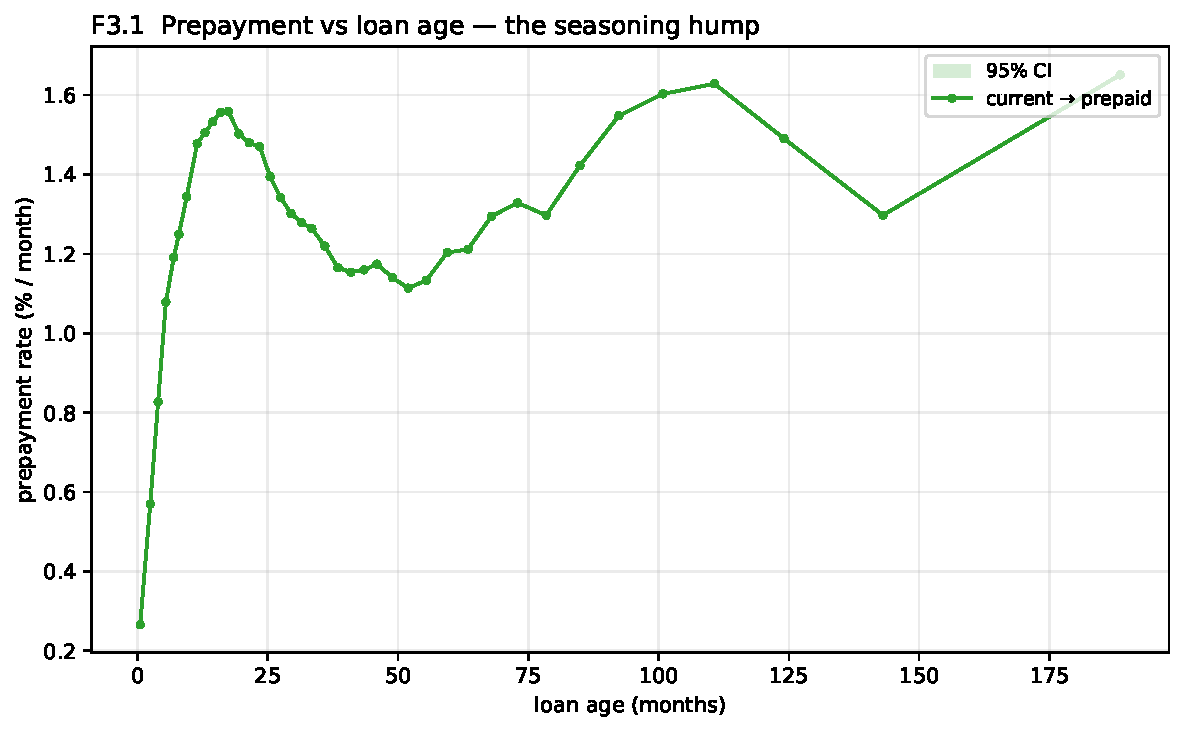
\includegraphics[width=0.8\textwidth]{figs/F3.1_prepay_age.pdf}
\caption[Empirical prepayment hazard by loan age]{Empirical prepayment
hazard by loan age (equal-population buckets, Wilson 95\% intervals):
the seasoning hump.}\label{fig:hazard-age}
\end{figure}

\begin{figure}[htbp]\centering
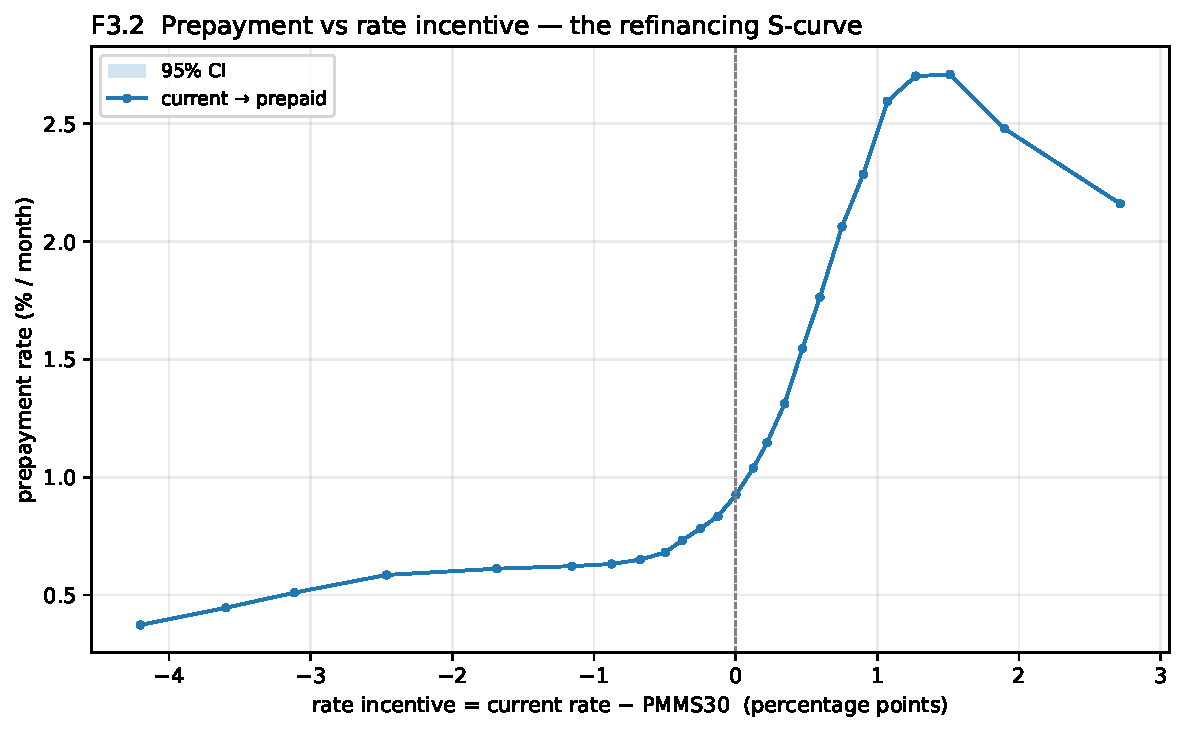
\includegraphics[width=0.8\textwidth]{figs/F3.2_prepay_incentive.pdf}
\caption[Empirical prepayment hazard by refinancing incentive]{Empirical
prepayment hazard by refinancing incentive: the S-curve, with burnout
beyond $+1.5$\,pp.}\label{fig:hazard-incentive}
\end{figure}

\begin{figure}[htbp]\centering
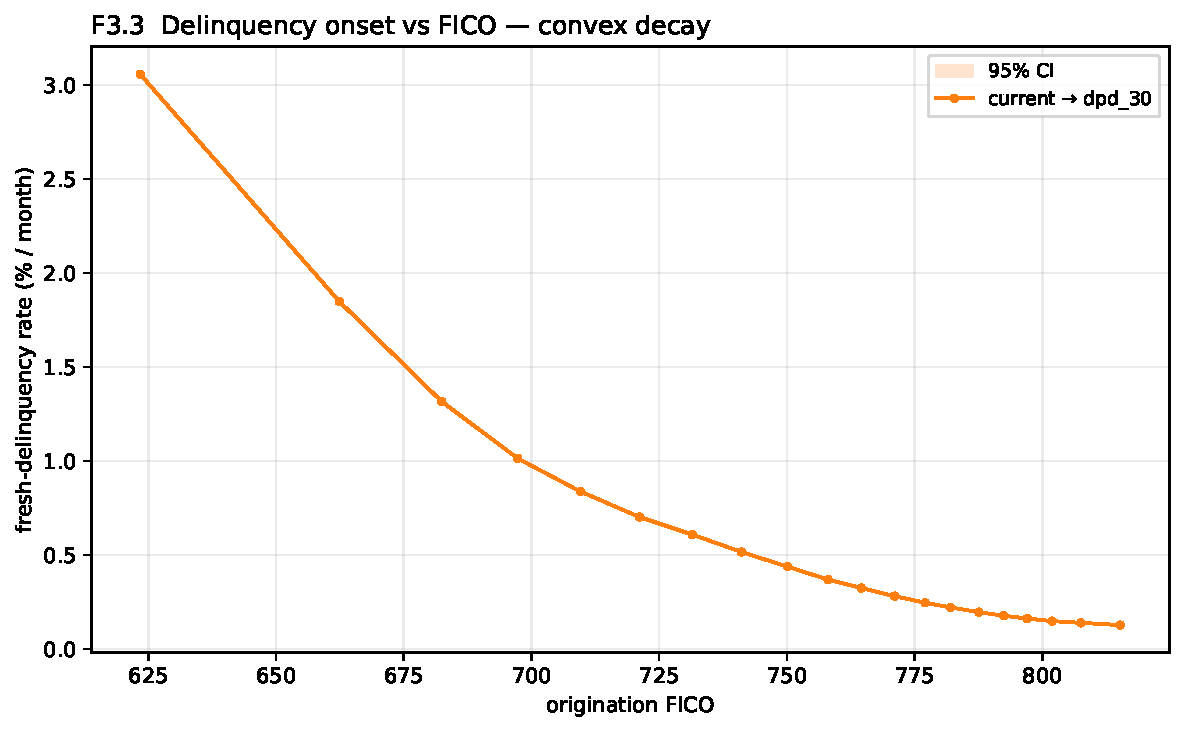
\includegraphics[width=0.8\textwidth]{figs/F3.3_delinq_fico.pdf}
\caption[Empirical 30\,DPD entry hazard by origination credit
score]{Empirical 30\,DPD entry hazard by origination credit score:
convex decay.}\label{fig:hazard-fico}
\end{figure}

\subsection{Interactions: the case against additivity}
\label{subsec:data-eda-interactions}

A linear-\emph{additive} model could in principle be patched with
transformed single-variable terms; interactions are what it cannot
absorb.  On a credit-score~$\times$~LTV grid
(Figure~\ref{fig:interaction-ficoltv}), the monthly rate of entry
into delinquency ranges from $0.11\%$ (best scores, lowest leverage)
to $2.69\%$ (worst scores, highest leverage) --- and decisively, the
\emph{additive} credit-score gradient (worst-minus-best rate) grows
from $1.73$ percentage points at low LTV to $2.48$ at high LTV, a
$43\%$ increase; equivalently, the leverage effect is roughly
$8.5$ times larger for low-score than high-score borrowers.
Additivity forces this gradient to be constant; the violation sits
exactly in the low-score/high-leverage corner that drives credit
losses.  In the prepayment channel
(Figure~\ref{fig:interaction-incfico}), splitting the incentive
S-curve by credit-score tercile shows the in-the-money refinancing
response \emph{rising} with credit quality --- $2.36\%$ per month in
the lowest tercile against $3.01\%$ in the highest --- because
credit-constrained borrowers cannot exercise the option: the
incentive \emph{slope} itself depends on the score.  Finally, holding
loan age fixed at 12--36 months to strip out seasoning, the
delinquency hazard by origination cohort isolates a clean vintage
effect: the 2007 cohort peaks at $1.68\%$ per month against $0.47\%$
for calm cohorts --- a $3.6$-fold premium
(Figure~\ref{fig:vintage}) --- so the origination vintage is a
feature in its own right, not reducible to contemporaneous
covariates.

\begin{figure}[htbp]\centering
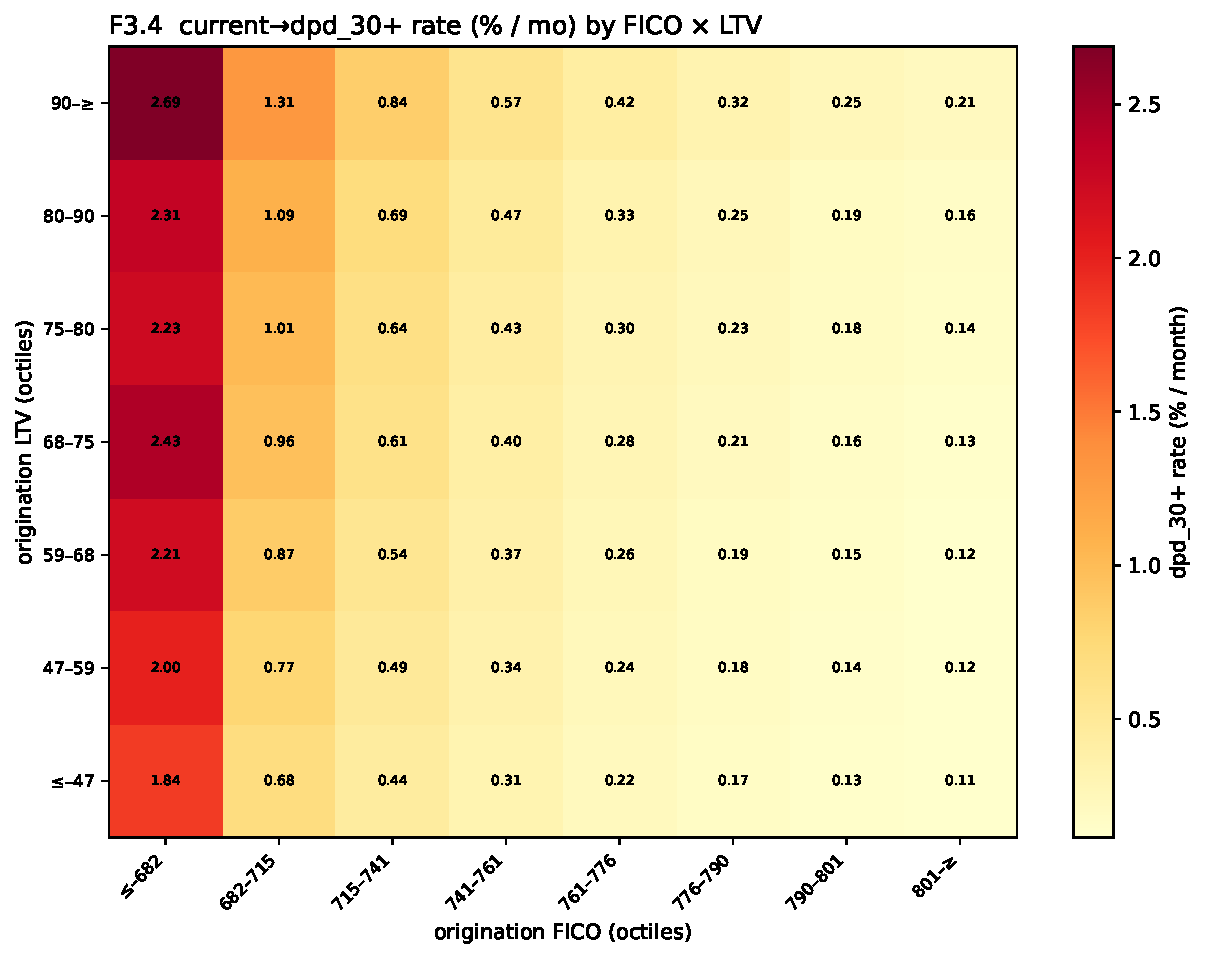
\includegraphics[width=0.78\textwidth]{figs/F3.4_fico_ltv_heatmap.pdf}
\caption[Monthly delinquency-entry rate on a credit-score $\times$ LTV
grid]{Monthly delinquency-entry rate on a credit-score $\times$ LTV grid
(equal-population bands): the additive credit-score gradient grows with
leverage --- additivity is misspecified.}\label{fig:interaction-ficoltv}
\end{figure}

\begin{figure}[htbp]\centering
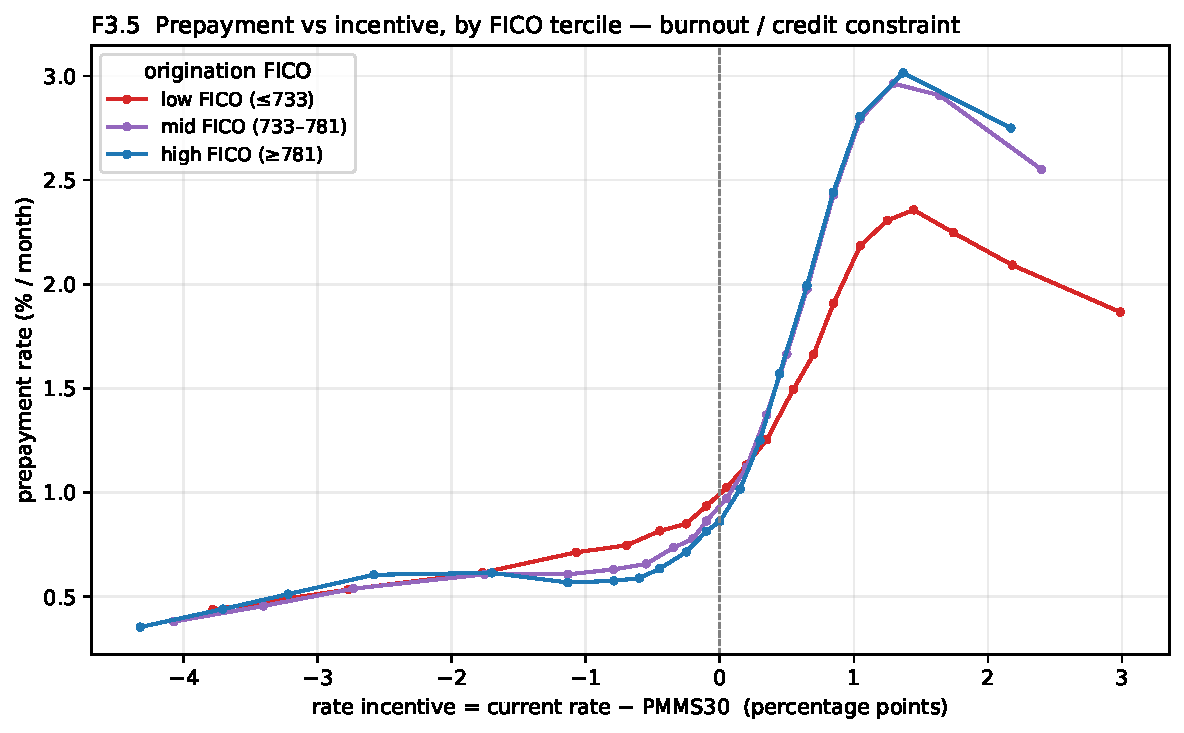
\includegraphics[width=0.8\textwidth]{figs/F3.5_incentive_fico.pdf}
\caption[The incentive S-curve by credit-score tercile]{The incentive
S-curve by credit-score tercile: the refinancing response to an
in-the-money option rises with credit
quality.}\label{fig:interaction-incfico}
\end{figure}

\begin{figure}[htbp]\centering
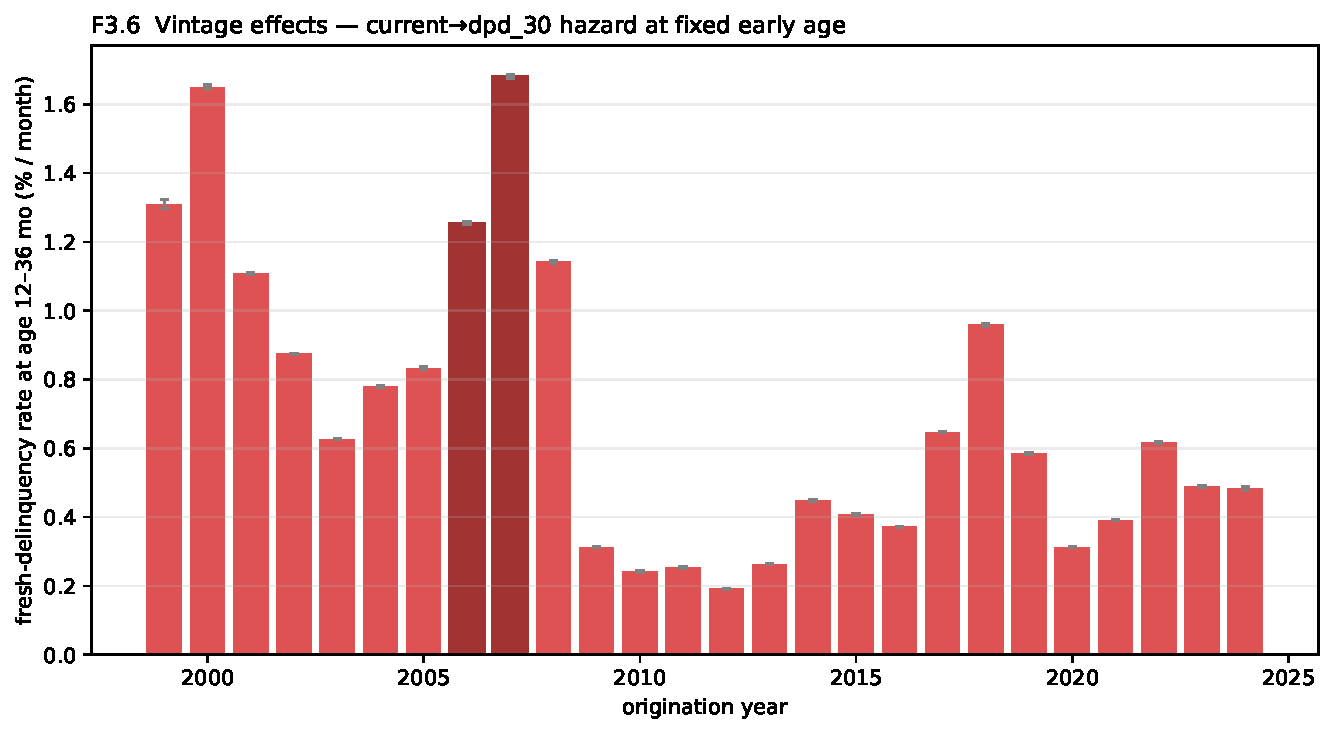
\includegraphics[width=0.8\textwidth]{figs/F3.6_vintage.pdf}
\caption[Delinquency hazard by origination cohort at fixed loan
age]{Delinquency hazard by origination cohort at fixed loan age
(12--36 months): the 2006--08 bubble vintages.}\label{fig:vintage}
\end{figure}

Taken together, the evidence points one way: monthly transition risk
depends on the covariates nonlinearly (the seasoning hump, the
incentive S-curve, convex credit-score decay) and interactively
(score$\times$leverage, incentive$\times$score, vintage).  A
linear-additive model should therefore underfit --- most severely on
prepayment, the channel combining the sharpest single-variable
nonlinearity with a first-order interaction --- and
Chapter~\ref{chap:results} tests precisely this.

% ────────────────────────────────────────────────────────────
\section{Comparison to Sirignano et al.\ (2021)}
\label{sec:data-comparison}

The dataset employed in the present study differs in several important
respects from the proprietary CoreLogic dataset used by
\citet{sirignano2021}, and these differences bear on the
interpretation of the results.

\citet{sirignano2021} draw on records for approximately 120 million
mortgages --- both prime and subprime --- originated across the United
States between January 1995 and June 2014, yielding approximately 3.5
billion loan-month observations.  The CoreLogic data encompass the
full spectrum of mortgage products, including fixed-rate,
adjustable-rate, hybrid, balloon, and interest-only loans, as well as
government-insured instruments.  Macro-economic covariates ---
zip-code-level house price indices from Zillow, county-level
unemployment rates from the Bureau of Labor Statistics, and the
Freddie Mac PMMS series --- are merged at the loan-month level within
the CoreLogic database.  The dataset is proprietary and cannot be
reproduced by independent researchers.

The Fannie Mae primary dataset, by contrast, is limited to
conventional fixed-rate fully-amortising loans and excludes both
subprime and government-insured products.  Macro-economic covariates
must be sourced and joined externally, as described in
Section~\ref{subsec:data-external}.  These differences have two
principal consequences.  First, the estimation sample is more
homogeneous in product mix; the nonlinear prepayment dynamics
associated with adjustable-rate burnout and subprime option exercise
--- prominent in \citeauthor{sirignano2021} --- are absent.  Second,
the absence of a subprime segment limits the range of credit-risk
outcomes observed; \citet{sirignano2021} report a median FICO score
of 630 for their subprime sub-sample against 730 for the prime
sub-sample, whereas the Fannie Mae population is concentrated at the
higher end of this credit-quality spectrum.

These limitations notwithstanding, the Fannie Mae dataset provides a
fully reproducible basis for the analysis.  The core methodological
contribution of \citet{sirignano2021} --- applying deep learning to a
multinomial competing-risks model of monthly loan-state transitions
--- transfers completely to the Fannie Mae panel.  The architecture,
estimation procedure, and evaluation framework described in subsequent
chapters are direct adaptations of that approach.  Table~\ref{tab:data-comparison}
summarises the key differences.

\begin{table}[htbp]
  \centering
  \small
  \begin{tabularx}{\textwidth}{@{} l X X @{}}
    \toprule
    \textbf{Dimension}
      & \textbf{Sirignano et al.\ (2021)}
      & \textbf{Present study} \\
    \midrule
    Data source
      & CoreLogic (proprietary)
      & Fannie Mae SFLP (public) \\[3pt]
    Total loans
      & ${\sim}120$ million
      & 57.6 million \\[3pt]
    Loan-month observations
      & ${\sim}3.5$ billion
      & 3.31 billion \\[3pt]
    Origination window
      & 1995--2014
      & 1999--2025 (full vintage set, reporting to 2025-12) \\[3pt]
    Products covered
      & Fixed, ARM, hybrid, balloon, IO
      & Fixed-rate, fully amortising only \\[3pt]
    Credit segments
      & Prime and subprime
      & Conventional (predominantly prime) \\[3pt]
    Macro covariates
      & Embedded (Zillow, BLS, PMMS)
      & External join required (FHFA HPI, PMMS) \\[3pt]
    Geographic detail
      & Full 5-digit zip code
      & 3-digit truncated zip; MSA \\[3pt]
    States modelled
      & Seven
      & Seven (identical mapping) \\[3pt]
    Reproducibility
      & Not publicly reproducible
      & Fully reproducible \\
    \bottomrule
  \end{tabularx}
  \caption[Comparison of the Fannie Mae SFLP dataset and the
  CoreLogic dataset used by Sirignano et al.\ (2021)]%
  {\textit{Comparison of the Fannie Mae SFLP primary dataset and the
  CoreLogic dataset used by \citet{sirignano2021}.}  CoreLogic counts
  are approximate as reported by the authors; Fannie Mae counts are
  measured on the assembled panel (Section~\ref{sec:data-summary}).}
  \label{tab:data-comparison}
\end{table}

%  to main.tex (after chapter2, before conclusions).
%
%  Required packages (add to the preamble of main.tex):
%      \usepackage{booktabs}
%      \usepackage{tabularx}
%      \usepackage{multirow}
%      \usepackage{natbib}   % or your preferred bib style
% ============================================================

\chapter{Data}
\label{chap:data}

% ────────────────────────────────────────────────────────────
\section{Data Source}
\label{sec:data-source}

This study employs the Fannie Mae Single-Family Loan Performance
(SFLP) dataset, a publicly available research dataset maintained by
the Federal National Mortgage Association (Fannie Mae) and updated on
a quarterly basis.  The dataset was originally released in April 2013
and contains origination and monthly performance records for a subset
of single-family conventional mortgage loans acquired by Fannie Mae
since January 2000.  New loan acquisitions and performance data are
added with an approximate four-month lag following the end of each
calendar quarter \citep{fanniemae2024}.

The data are organised as a \emph{loan-month panel}: each observation
corresponds to a single mortgage loan in a single monthly reporting
period, beginning at the month of acquisition and continuing until the
loan terminates through full prepayment, foreclosure, Real Estate
Owned (REO) disposition, or contractual maturity, or until the data
cut-off date.  This longitudinal structure is well-suited to the
competing-risks framing of \citet{sirignano2021}, which the present
study adapts to the Fannie Mae data.

Raw files are distributed as pipe-delimited CSV without a header row,
organised by acquisition quarter and identified by the convention
\texttt{YYYYQn.csv}.  Column identities are positional, fully
specified in the Fannie Mae Single-Family Loan Performance Data File
Layout and Glossary.  Each row contains 113 fields encoding static
origination attributes, dynamic monthly performance measures, and
post-termination expense and proceeds data.  The estimation sample
employed in this study is the \emph{complete} vintage set from a
single quarterly release: 104 acquisition-quarter files covering
cohorts from 2000Q1 onwards, with monthly reporting periods from
January 2000 through December 2025.  The assembled panel comprises
\textbf{3{,}312{,}456{,}883 loan-month observations across
57{,}562{,}668 loans} --- performance histories spanning four
interest-rate cycles, the 2008--11 foreclosure crisis, the COVID-era
forbearance episode, and the 2022--23 rate shock.

\subsection{From raw files to the estimation panel}
\label{subsec:data-pipeline}

Three distinct concepts in this dataset are colloquially called a
``quarter,'' and distinguishing them prevents the most common
assembly errors.  The \emph{acquisition vintage} identifies a file:
each \texttt{YYYYQn.csv} contains the loans Fannie Mae acquired in
that quarter, carrying their entire subsequent monthly history, and a
loan appears in exactly one file --- so concatenating all files
assembles the full sample with no duplication.  The \emph{monthly
reporting period} identifies a row, and this time dimension --- not
redundancy --- is why the dataset is large.  The \emph{release}
identifies the download: Fannie Mae republishes the entire dataset
quarterly with extended histories, so all files must come from one
release lest vintages carry inconsistent right-censoring dates; an
ingestion audit verifies a uniform cut-off across all 104 files.

Because no single file fits in memory ($\sim$800\,GB of raw CSV in
total), a six-stage pipeline converts the files into a compressed,
columnar store queried out of core: an integrity audit, streaming
conversion, type and sentinel cleaning, construction of the
transition panel with the outcome variable of
Section~\ref{sec:data-outcome}, sampling utilities, and a
reconciliation step that verifies row counts against the raw files.
Columnar storage means a query touching six of the 113 fields reads
roughly five per cent of the bytes, which is what makes the
full-panel descriptive statistics and exploratory analysis of
Sections~\ref{sec:data-summary} and~\ref{sec:data-eda}
computationally cheap.

% ────────────────────────────────────────────────────────────
\section{Population and Eligibility}
\label{sec:data-population}

The primary dataset is not a census of all loans in Fannie Mae's
guarantee book; it is a curated research sample subject to documented
eligibility and exclusion criteria \citep{fanniemae2024}.  The
population is restricted to fixed-rate, fully amortising,
full-documentation single-family conventional mortgage loans with
original terms of at least five years and less than 35 years,
originated on or after 1 January 1999 and acquired by Fannie Mae on
or after 1 January 2000.

A number of product types are explicitly excluded.  Adjustable-rate
mortgages, interest-only loans, balloon-amortisation mortgages, and
loans carrying prepayment penalties are absent from the dataset.
Also excluded are loans with original loan-to-value (LTV) ratios
exceeding 97 per cent, Alt-A and other reduced-documentation
products, government-insured loans (FHA and VA), loans subject to
long-term standby commitments or third-party risk-sharing
arrangements other than primary mortgage insurance, and loans
acquired on a negotiated bulk basis.  Loans with non-standard payment
due dates and loans that liquidated in the same month as acquisition
are similarly excluded.  Fannie Mae's Home Affordable Refinance
Program (HARP) loans are likewise absent from the primary dataset;
when a loan in the primary dataset was subsequently refinanced through
HARP, its termination is recorded as a standard prepayment, and its
post-refinance performance is not tracked here.  This is discussed
further in Section~\ref{sec:data-outcome}.

These restrictions yield a sample of conventionally underwritten
fixed-rate mortgages broadly representative of the agency conventional
loan market under post-crisis underwriting standards.  The exclusion
of adjustable-rate and interest-only products limits the range of
prepayment incentive dynamics captured relative to the full-spectrum
dataset used by \citet{sirignano2021}; this is discussed in
Section~\ref{sec:data-comparison}.  Table~\ref{tab:eligibility}
summarises the principal eligibility criteria and exclusions.

\begin{table}[htbp]
  \centering
  \small
  \begin{tabularx}{\textwidth}{@{} l X @{}}
    \toprule
    \textbf{Criterion} & \textbf{Requirement / Exclusion} \\
    \midrule
    Origination date      & On or after 1 January 1999 \\[2pt]
    Acquisition date      & On or after 1 January 2000 \\[2pt]
    Product type          & Fixed-rate, fully amortising only \\[2pt]
    Loan term             & $5 \leq \mathrm{term} < 35$ years at origination \\[2pt]
    Documentation         & Full documentation only \\[2pt]
    LTV at origination    & $\leq 97\%$ \\[4pt]
    \emph{Excluded: product}      & ARM, interest-only, balloon,
                                    prepayment-penalty loans \\[2pt]
    \emph{Excluded: credit class} & Alt-A, reduced-documentation,
                                    streamlined processing \\[2pt]
    \emph{Excluded: guarantee}    & Government-insured (FHA, VA) loans \\[2pt]
    \emph{Excluded: structure}    & Long-term standby commitments;
                                    bulk acquisitions; lender-recourse
                                    loans (except primary MI) \\[2pt]
    \emph{Excluded: programme}    & HARP and Refi Plus loans \\[2pt]
    \emph{Excluded: payment}      & Bi-weekly and non-first-of-month
                                    due dates \\[2pt]
    \emph{Excluded: timing}       & Loans liquidated in month of
                                    acquisition \\
    \bottomrule
  \end{tabularx}
  \caption[Eligibility criteria for the Fannie Mae SFLP primary dataset]%
  {\textit{Eligibility criteria for the Fannie Mae SFLP primary
  dataset.}  Source: Fannie Mae Single-Family Loan Performance
  Dataset FAQs \citep{fanniemae2024}.}
  \label{tab:eligibility}
\end{table}

% ────────────────────────────────────────────────────────────
\section{Variables}
\label{sec:data-variables}

The 113 fields in each monthly observation can be organised into three
functional groups: static origination attributes, dynamic monthly
performance attributes, and post-termination resolution data.  The
model uses a subset of these fields as covariates.  Two fields --- the
Current Loan Delinquency Status and the Zero Balance Code --- serve as
the primary inputs from which the outcome variable is constructed.

% ────────────────────────────────
\subsection{Origination Attributes}
\label{subsec:data-origination}

Static origination attributes are recorded at loan delivery and do
not change over the life of the loan absent a modification.  The
borrower's FICO credit score at origination is available for both the
primary borrower and, where applicable, a co-borrower; prior to the
January 2015 dataset release only the lower of the two scores was
disclosed, and a missingness indicator is constructed accordingly.
Continuous origination covariates include the original
debt-to-income (DTI) ratio, original LTV ratio, original combined LTV
(CLTV, which incorporates subordinate liens), original unpaid
principal balance (UPB), original interest rate, and original loan
term in months.  Categorical origination attributes include the
acquisition channel (retail, broker, or correspondent), loan purpose
(purchase, rate-term refinance, or cash-out refinance), property type,
occupancy status (primary residence, second home, or investment
property), property state, Metropolitan Statistical Area (MSA), and
three-digit truncated zip code.  The truncation of the zip code
reflects borrower privacy considerations; full zip codes are not
disclosed in the dataset \citep{fanniemae2024}.

% ────────────────────────────────
\subsection{Dynamic Performance Attributes}
\label{subsec:data-performance}

Dynamic performance attributes are updated in each monthly reporting
period.  The current actual unpaid principal balance reflects the
outstanding loan balance at each point in time.  Loan age, measured
in months from the first payment date, and the remaining months to
legal maturity are derived from the contractual amortisation schedule.
The current interest rate reflects the applicable note rate, updated
when a modification changes the loan terms.

Two dynamic fields jointly determine the outcome variable.  The
\textbf{Current Loan Delinquency Status} reports the number of missed
monthly payments as a two-character code: \texttt{00} denotes a
current loan; \texttt{01}, \texttt{02}, and codes \texttt{03} and
above denote 30-, 60-, and 90-or-more-day delinquencies respectively;
and \texttt{XX} denotes an unavailable status.  The \textbf{Zero
Balance Code} is populated exclusively in the terminal monthly
observation and classifies the manner of loan termination into nine
categories, distinguishing between voluntary prepayments, third-party
foreclosure sales, short sales, repurchases, REO dispositions, note
sales, and non-credit removals.  (The dataset also carries a 24-month
payment-history string; it is not used as a model input here, since
the current state and loan-level covariates already summarise the
information the transition model conditions on.)

% ────────────────────────────────
\subsection{Externally Sourced Covariates}
\label{subsec:data-external}

A small, fixed set of external macroeconomic series is joined to the
loan-level panel at feature-construction time (the stored panel
itself is never rewritten); Table~\ref{tab:macrovars} summarises the
sources.  The Freddie Mac Primary Mortgage Market Survey (PMMS)
weekly fixed-rate series, aggregated to calendar-month means, supplies
the prevailing market mortgage rate from which the \emph{rate
incentive} of Equation~\eqref{eq:incentive} is computed --- the
refinancing option value, the primary driver of prepayment behaviour
in the empirical mortgage literature
\citep{schwartz1989,sirignano2021}.  Unemployment rates enter at both
national (Bureau of Labor Statistics) and state level, the latter
because the cross-sectional dispersion in labour-market conditions
(Nevada versus Texas in 2009) is precisely the variation a national
series cannot supply.  House prices enter through the Freddie Mac
House Price Index at national and state level, from which the
mark-to-market loan-to-value ratio of Equation~\eqref{eq:mtmltv} ---
the principal determinant of the default option value
\citep{deng2000} --- and the trailing twelve-month house-price change
are constructed.  The ten-year Treasury yield completes the set.

Each series is joined with a \emph{publication lag} reflecting when
the value was actually observable: rates are published in real time
(no lag), month-$t$ unemployment is released early in month $t{+}1$
(one-month lag), and the house-price index roughly two months after
the reference month (two-month lag).  Final-revision series are used
rather than real-time vintages --- a stated limitation, standard for
historical studies.  Where a state-level value is unavailable
(territories; series start dates) the national value substitutes,
with an indicator flag carried as a model feature.

\begin{table}[htbp]
  \centering
  \small
  \begin{tabularx}{\textwidth}{@{} l l l l c @{}}
    \toprule
    \textbf{Variable} & \textbf{Source} & \textbf{Geography}
      & \textbf{Monthly value} & \textbf{Lag} \\
    \midrule
    30-yr mortgage rate & Freddie Mac PMMS & national & month mean & 0\,m \\
    10-yr Treasury yield & FRED \texttt{DGS10} & national & month mean & 0\,m \\
    Unemployment rate & BLS (via FRED) & national + state & as published & 1\,m \\
    House-price index & Freddie Mac FMHPI & national + state & as published & 2\,m \\
    \bottomrule
  \end{tabularx}
  \caption[External macroeconomic covariates and join conventions]%
  {\textit{External macroeconomic covariates and join conventions.}
  A loan-month at calendar month $t$ is joined to the macro value of
  month $t-\ell$, where $\ell$ is the publication lag.  Seasonally
  adjusted versions are used throughout.}
  \label{tab:macrovars}
\end{table}

As a check on the incentive variable, a market-rate proxy derived
from the panel itself --- the average note rate of loans originated
in each calendar month --- tracks the PMMS series with correlation
$0.991$, root-mean-square deviation $0.198$ percentage points, and
mean absolute deviation $0.147$ percentage points, with a mean gap of
essentially zero.  The PMMS-based incentive is the primary feature;
the panel-derived proxy is retained as a robustness alternative,
demonstrating that the incentive variable is not an artefact of one
data source.

% ────────────────────────────────────────────────────────────
\section{Outcome Variable}
\label{sec:data-outcome}

Following \citet{sirignano2021}, the outcome variable is a categorical
measure of mortgage state in month $t+1$, conditional on the loan's
state and covariate vector in month $t$.  Seven mutually exclusive
states are defined: \emph{Current}, \emph{30 Days Past Due}
(30\,DPD), \emph{60 Days Past Due} (60\,DPD), \emph{90+ Days Past
Due} (90+\,DPD), \emph{Foreclosure}, \emph{Real Estate Owned} (REO),
and \emph{Prepaid}.

State assignment for each loan-month observation follows a
deterministic hierarchy.  When the Zero Balance Code is present ---
indicating the terminal observation for the loan --- the termination
type is mapped to the Foreclosure, REO, or Prepaid absorbing state as
shown in Table~\ref{tab:state-mapping}.  When the Zero Balance Code is
absent, the delinquency status field governs: codes \texttt{00}
through \texttt{03} and above map to Current, 30\,DPD, 60\,DPD, and
90+\,DPD respectively, while \texttt{XX} is treated as missing.  The
state in month $t+1$ is obtained by a window lead over the reporting
period dimension, partitioned by loan identifier.  Loans whose final
observation falls at or before the data cut-off without a recorded
termination event receive a censored indicator and are excluded from
the labelled target.

Regarding HARP loans: as noted in Section~\ref{sec:data-population},
any loan in the primary dataset that was refinanced through the
HARP programme terminates with a Zero Balance Code of \texttt{01}
(prepaid) at the moment of refinancing and is therefore treated as a
standard prepayment in the outcome variable.  This approximation is
defensible given that the loan is extinguished from Fannie Mae's
credit exposure in either case, though it may marginally overstate
the rate-incentive sensitivity of the prepayment hazard during the
period of peak HARP activity (approximately 2009--2013).

\begin{table}[htbp]
  \centering
  \small
  \begin{tabularx}{\textwidth}{@{} l l l X @{}}
    \toprule
    \textbf{State} & \textbf{Source field} & \textbf{Condition}
      & \textbf{Economic interpretation} \\
    \midrule
    Current
      & Delinquency Status & \texttt{= 00}
      & Borrower is contractually current on all payments. \\[3pt]
    30\,DPD
      & Delinquency Status & \texttt{= 01}
      & One missed monthly payment. \\[3pt]
    60\,DPD
      & Delinquency Status & \texttt{= 02}
      & Two consecutive missed monthly payments. \\[3pt]
    90+\,DPD
      & Delinquency Status & \texttt{$\geq$ 03}
      & Three or more missed payments; serious delinquency. \\[3pt]
    Foreclosure
      & Zero Balance Code  & \texttt{02, 03, 15,}
      & Credit-loss termination: third-party sale, short sale, \\
      &                    & \texttt{97, 98}
      & note sale, or credit-event repurchase. \\[3pt]
    REO
      & Zero Balance Code  & \texttt{= 09}
      & Fannie Mae acquires ownership of the property. \\[3pt]
    Prepaid
      & Zero Balance Code  & \texttt{01, 06, 16,}
      & Full payoff, contractual maturity, repurchase, \\
      &                    & \texttt{96}
      & or non-credit removal (including HARP exits). \\
    \bottomrule
  \end{tabularx}
  \caption[Mapping of Fannie Mae data fields to the seven-state
  outcome variable]%
  {\textit{Mapping of Fannie Mae data fields to the seven-state
  outcome variable.}  The Zero Balance Code is populated only in the
  terminal monthly observation; the Delinquency Status governs state
  assignment in all non-terminal periods.}
  \label{tab:state-mapping}
\end{table}

One structural feature of this dataset deserves emphasis: because the
Foreclosure, REO, and Prepaid states are derived from the Zero
Balance Code --- populated only in a loan's final observation ---
these three states are \emph{absorbing}.  There is no ongoing ``in
foreclosure'' monthly status as in the CoreLogic data of
\citet{sirignano2021}, where loans in formal foreclosure are observed
month by month and occasionally return to performing status.  The
origin set here therefore comprises the four live states (Current
through 90+\,DPD) while destinations span all seven: the transition
matrix is $4\times 7$ rather than $7\times 7$
(Section~\ref{sec:meth-model}).  Within the live states the data are
rich in both directions --- delinquency deepens at most one bucket
per month, but cures can jump multiple buckets, and a meaningful
fraction of seriously delinquent loans return to current.  The
seven-state formulation captures this in a way that a binary
default-versus-prepayment classification would obscure, and the
empirical monthly transition matrix derived from each training window
serves as the floor benchmark for the model comparison
(Section~\ref{subsec:meth-empirical}).

% ────────────────────────────────────────────────────────────
\section{Panel Composition and Summary Statistics}
\label{sec:data-summary}

The assembled panel comprises 3{,}312{,}456{,}883 loan-month
observations across 57{,}562{,}668 loans in 104 acquisition-vintage
partitions, with reporting months from January 2000 through December
2025.  Table~\ref{tab:stateshares} reports the distribution of
loan-months across the seven states.  Two features dominate.  First,
extreme class imbalance: the Current state accounts for $96.28\%$ of
all loan-months, while the credit-event terminals occur at roughly
one in ten thousand observations --- the empirical fact behind both
the importance-weighted thinning of training data
(Section~\ref{sec:meth-design}) and the Laplace smoothing of the
empirical benchmark (Section~\ref{subsec:meth-empirical}).  Second,
the rare states are nonetheless abundantly populated in absolute
terms (REO alone contributes roughly half a million loan-months),
which is what permits stable estimation of rare-transition
probabilities at this scale.

\begin{table}[htbp]
  \centering
  \small
  \begin{tabular}{l r @{\qquad\qquad} l r}
    \toprule
    \textbf{State} & \textbf{Share} & \textbf{State} & \textbf{Share} \\
    \midrule
    Current  & 96.28\,\% & 60\,DPD     & 0.31\,\%   \\
    Prepaid  & 1.25\,\%  & REO         & 0.014\,\%  \\
    30\,DPD  & 1.15\,\%  & Foreclosure & 0.0067\,\% \\
    90+\,DPD & 0.98\,\%  &             &            \\
    \bottomrule
  \end{tabular}
  \caption[Distribution of loan-months across the seven states]%
  {\textit{Distribution of loan-months across the seven states},
  full panel, 2000--2025 (3.31 billion loan-months).}
  \label{tab:stateshares}
\end{table}

Pooled over time, the monthly transition rates out of Current are
$1.27\%$ to Prepaid and $0.64\%$ to 30\,DPD.  The pooling, however,
hides the economics: Figure~\ref{fig:transitionrates} plots the
monthly series over 2000--2025, displaying the 2003 and 2020--21
refinancing waves in the prepayment rate, the 2008--11 default wave
in the delinquency rates, and the sharp 2022--23 collapse in
prepayments as market rates rose.  These regime shifts --- rather
than any single structural break --- are the empirical justification
for the rolling backtest design of Section~\ref{sec:meth-design}.
During 2020--21 the delinquency-status codes additionally reflect
COVID-era forbearance, which manifests as unusual persistence in
delinquency states followed by elevated cure rates; no special
treatment is applied, but results involving those years are read with
this in mind.

\begin{figure}[htbp]\centering
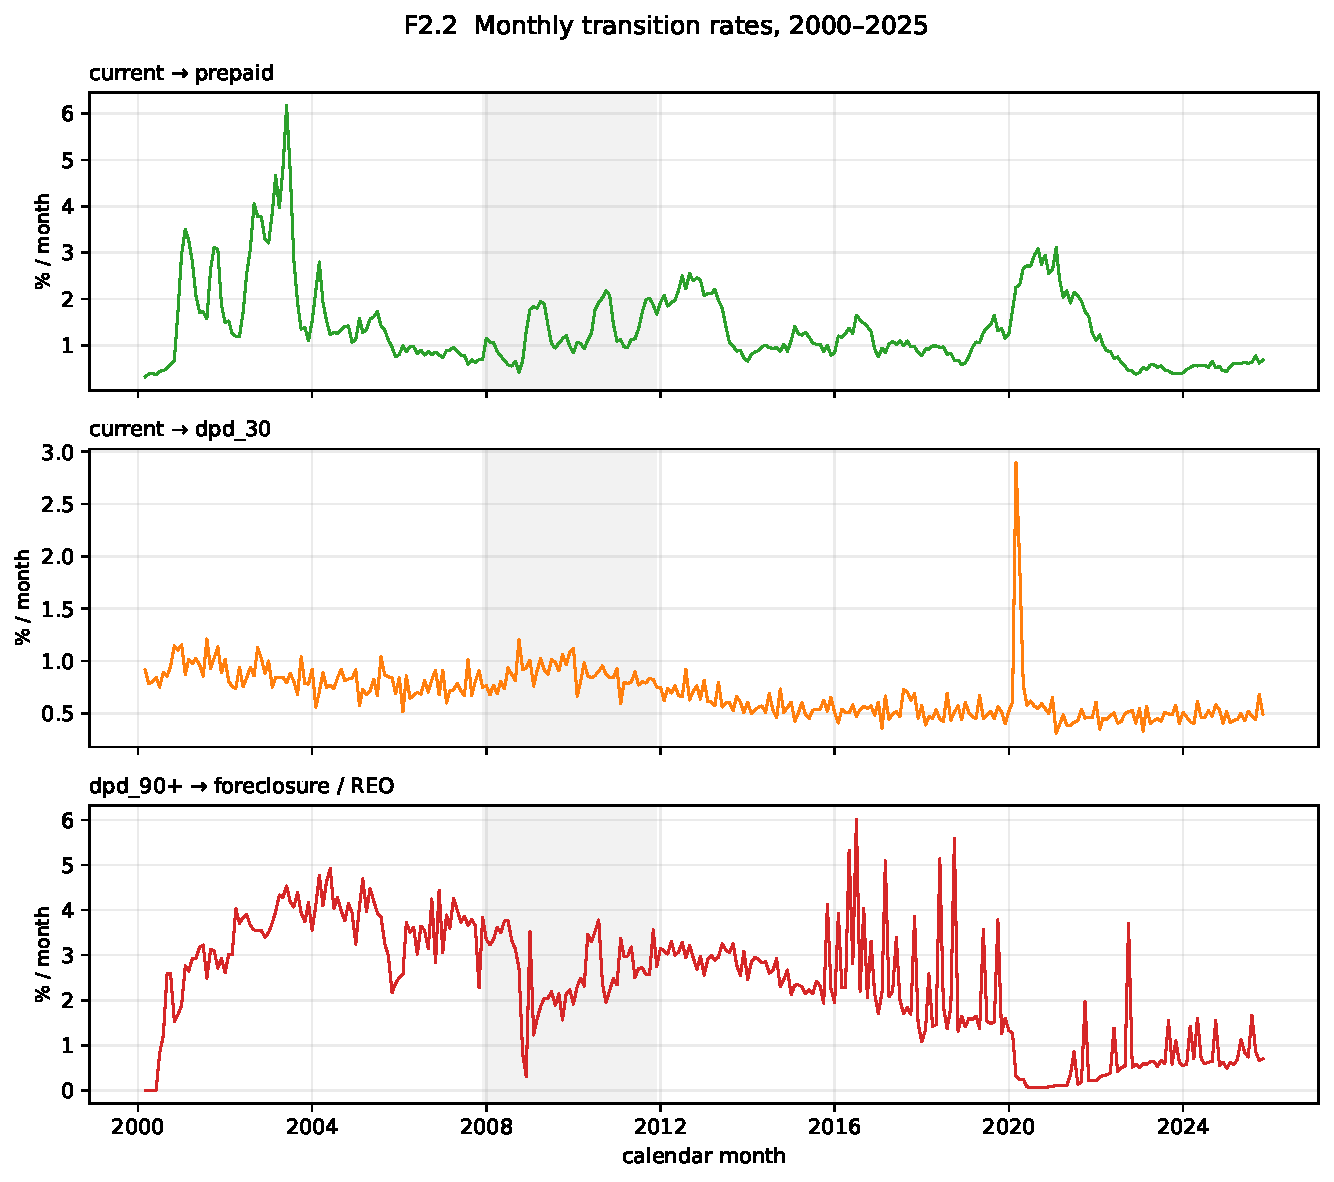
\includegraphics[width=0.9\textwidth]{figs/F2.2_transition_rates.pdf}
\caption[Monthly transition rates out of the Current state]{Monthly
transition rates out of the Current state, 2000--2025: prepayment and
entry into 30\,DPD (left axis), serious-delinquency terminations
(right axis).  Vertical shading marks the 2008--11 crisis and the
2020--21 forbearance episode.}\label{fig:transitionrates}
\end{figure}

\begin{table}[htbp]\centering\small
\caption[Summary statistics of model covariates]{Summary statistics of
the continuous model covariates over the full panel: null rate, mean,
standard deviation, and the min/1st/25th/50th/75th/99th/max
percentiles.}\label{tab:covariate-summary}
\resizebox{\textwidth}{!}{% Source: outputs/tables/eda/T1.2_covariate_summary_continuous.tex (full-panel
% Stage-6 QA). Tabular-only; wrap in \resizebox in chapter3.tex. Caption+label there.
\begin{tabular}{lrrrrrrrrrrl}
\toprule
column & null\_rate & mean & std & min & p01 & p25 & median & p75 & p99 & max & log\_flagged \\
\midrule
Original Interest Rate & 0 & 4.71882 & 1.32648 & 1.5 & 2.36602 & 3.62711 & 4.62688 & 5.75 & 7.85794 & 16.5 & False \\
Current Interest Rate & 0.012707 & 4.68763 & 1.32523 & 0 & 2.28982 & 3.625 & 4.60188 & 5.75 & 7.83746 & 13.5 & False \\
Original UPB & 0 & 199755 & 121639 & 1000 & 38809.4 & 109817 & 170562 & 262260 & 596156 & 2.326e+06 & True \\
Current Actual UPB & 0 & 159715 & 124113 & 0 & 0 & 71875.9 & 134287 & 224204 & 564970 & 2.86e+06 & True \\
Original Loan Term & 0 & 306.643 & 82.0617 & 36 & 120 & 202.959 & 360 & 360 & 360 & 360 & False \\
Loan Age & 0.01272 & 46.8107 & 42.4782 & -3 & 0 & 15 & 34.9747 & 65.8525 & 188.817 & 322 & False \\
Remaining Months to Maturity & 0.027474 & 252.795 & 97.4912 & 0 & 22.5446 & 167.472 & 294.279 & 335.84 & 359 & 480 & False \\
Original Loan-to-Value (LTV) & 0 & 69.7447 & 17.8489 & 1 & 21.1656 & 59.0522 & 74.5451 & 80 & 97 & 105 & False \\
Original Combined LTV (CLTV) & 0.003362 & 70.4277 & 17.9251 & 1 & 21.6837 & 59.7414 & 75 & 80 & 97 & 199 & False \\
Debt-to-Income (DTI) & 0.014108 & 33.3364 & 11.2275 & 0 & 9.02377 & 25 & 33.6755 & 41.9385 & 60.056 & 64 & False \\
fico\_orig & 0.002844 & 746.693 & 52.418 & 300 & 603.635 & 712.774 & 759.539 & 788.96 & 817.552 & 850 & False \\
fico\_co & 0.515382 & 754.702 & 49.6835 & 300 & 611.863 & 725.849 & 768.606 & 793.443 & 818.68 & 850 & False \\
Mortgage Insurance Percentage & 0.810875 & 24.1429 & 7.26184 & 0.12 & 6 & 22.29 & 25 & 30 & 35 & 50 & False \\
Number of Borrowers & 0.000119 & 1.55013 & 0.514524 & 1 & 1 & 1 & 2 & 2 & 2 & 10 & False \\
Number of Units & 0 & 1.03643 & 0.248099 & 1 & 1 & 1 & 1 & 1 & 2 & 4 & False \\
\bottomrule
\end{tabular}
}
\end{table}

% ────────────────────────────────────────────────────────────
\section{Exploratory Evidence: Nonlinearity and Interactions}
\label{sec:data-eda}

Before any model is fitted, the case that nonlinear modelling is
\emph{needed} can be made by counting alone.  The instrument is the
empirical hazard curve: bucket a covariate into equal-population
bins and plot the realised one-month transition rate per bin, with
Wilson 95\% confidence intervals.  Because each curve is a single
out-of-core aggregation over the columnar panel, the entire
programme runs in minutes.

\subsection{Single-covariate nonlinearity}
\label{subsec:data-eda-single}

Three hazard curves carry the argument.
\emph{Prepayment versus loan age}
(Figure~\ref{fig:hazard-age}): the rate rises from $0.27\%$ per month
at origination to a peak of $1.56\%$ at approximately 17 months of
age, then decays to $1.11\%$ by month 52 --- the classic
``seasoning hump,'' strongly non-monotone, with a secondary late-life
rise among long-surviving loans.  \emph{Prepayment versus the
refinancing incentive} (Figure~\ref{fig:hazard-incentive}): the rate
is flat at $0.4$--$0.6\%$ per month while the option is out of the
money, turns up sharply through zero, peaks at $2.71\%$ near
$+1.5$ percentage points of incentive, and falls back to $2.16\%$ by
$+2.7$ --- a roughly sevenfold range containing both an inflection
and a turning point, reproducing the flagship nonlinearity of
\citet{sirignano2021} on this cleaner credit box.
\emph{Delinquency versus credit score}
(Figure~\ref{fig:hazard-fico}): the entry rate into 30\,DPD falls
twenty-four-fold, from $3.06\%$ per month at FICO ${\approx}623$ to
$0.13\%$ at FICO ${\approx}815$, and the decay is convex --- the
slope in the low-score half is roughly $3.7$ times that in the
high-score half.  None of the three shapes is representable by a
linear term.

\begin{figure}[htbp]\centering
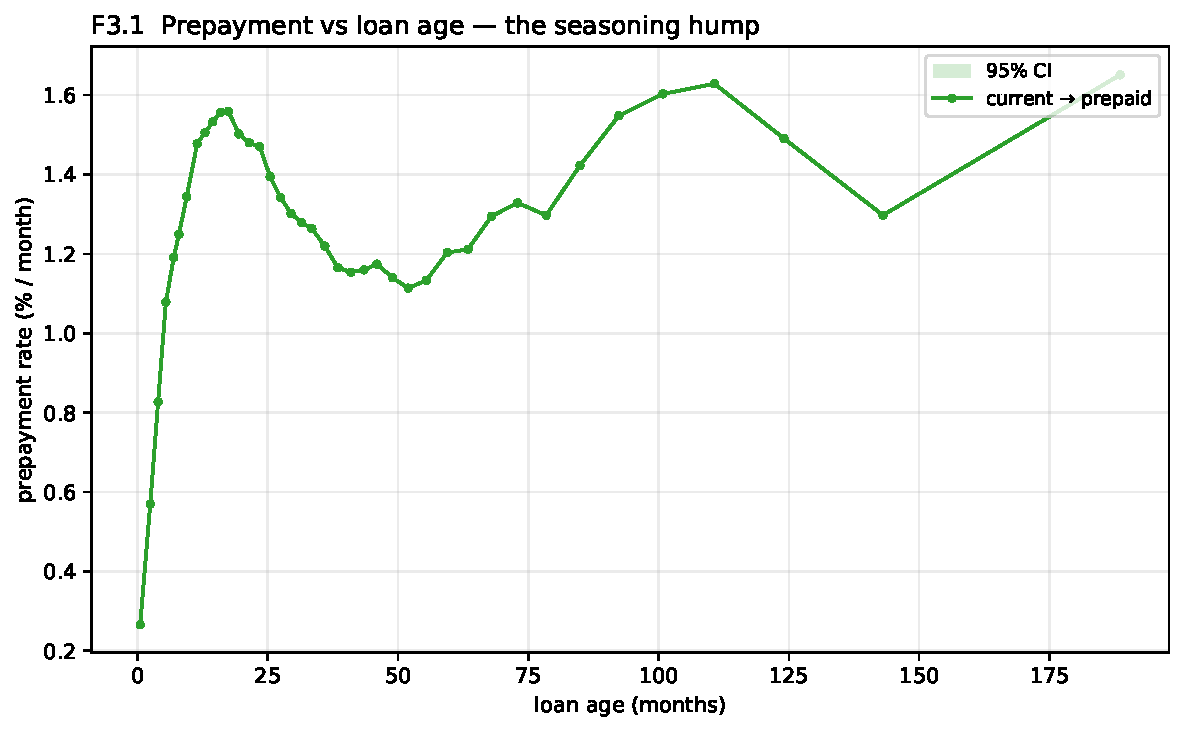
\includegraphics[width=0.8\textwidth]{figs/F3.1_prepay_age.pdf}
\caption[Empirical prepayment hazard by loan age]{Empirical prepayment
hazard by loan age (equal-population buckets, Wilson 95\% intervals):
the seasoning hump.}\label{fig:hazard-age}
\end{figure}

\begin{figure}[htbp]\centering
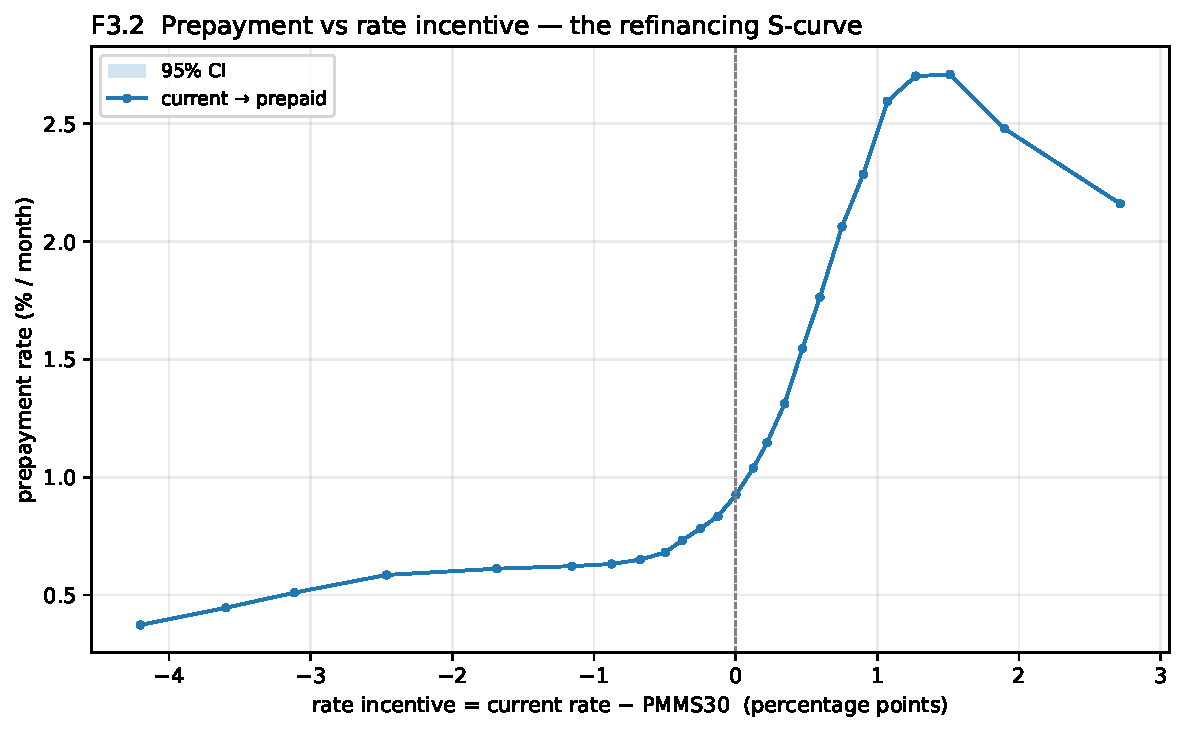
\includegraphics[width=0.8\textwidth]{figs/F3.2_prepay_incentive.pdf}
\caption[Empirical prepayment hazard by refinancing incentive]{Empirical
prepayment hazard by refinancing incentive: the S-curve, with burnout
beyond $+1.5$\,pp.}\label{fig:hazard-incentive}
\end{figure}

\begin{figure}[htbp]\centering
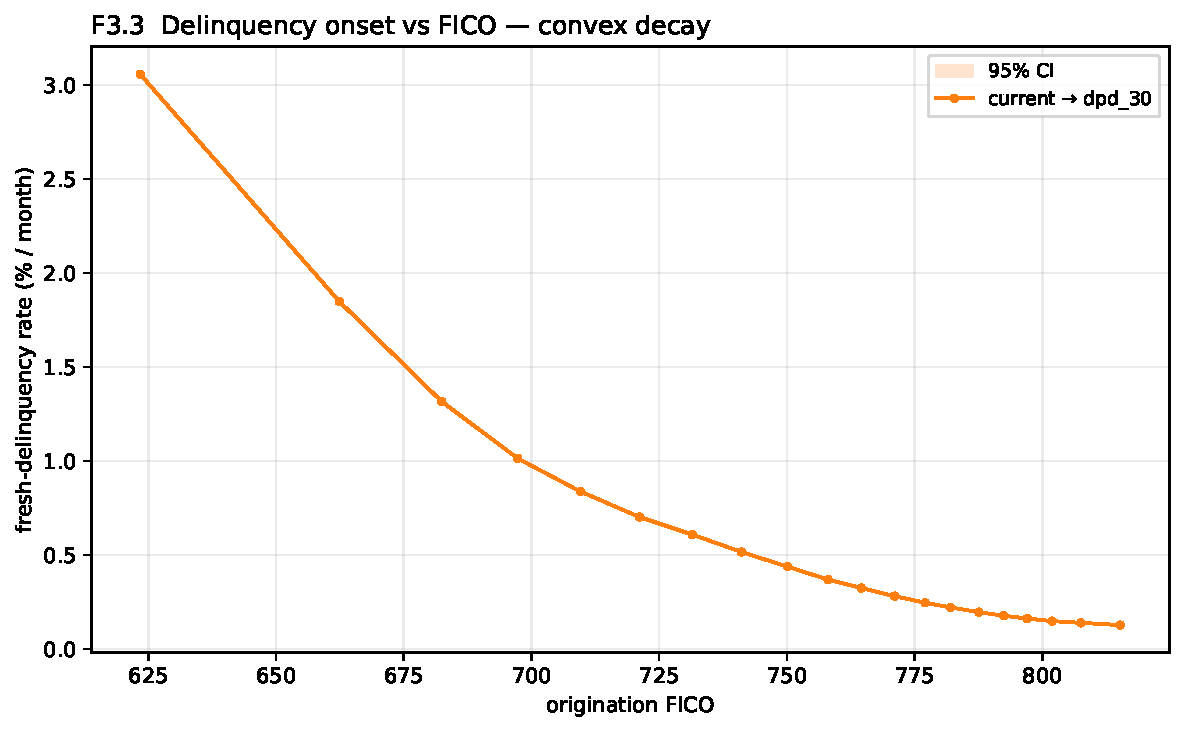
\includegraphics[width=0.8\textwidth]{figs/F3.3_delinq_fico.pdf}
\caption[Empirical 30\,DPD entry hazard by origination credit
score]{Empirical 30\,DPD entry hazard by origination credit score:
convex decay.}\label{fig:hazard-fico}
\end{figure}

\subsection{Interactions: the case against additivity}
\label{subsec:data-eda-interactions}

A linear-\emph{additive} model could in principle be patched with
transformed single-variable terms; interactions are what it cannot
absorb.  On a credit-score~$\times$~LTV grid
(Figure~\ref{fig:interaction-ficoltv}), the monthly rate of entry
into delinquency ranges from $0.11\%$ (best scores, lowest leverage)
to $2.69\%$ (worst scores, highest leverage) --- and decisively, the
\emph{additive} credit-score gradient (worst-minus-best rate) grows
from $1.73$ percentage points at low LTV to $2.48$ at high LTV, a
$43\%$ increase; equivalently, the leverage effect is roughly
$8.5$ times larger for low-score than high-score borrowers.
Additivity forces this gradient to be constant; the violation sits
exactly in the low-score/high-leverage corner that drives credit
losses.  In the prepayment channel
(Figure~\ref{fig:interaction-incfico}), splitting the incentive
S-curve by credit-score tercile shows the in-the-money refinancing
response \emph{rising} with credit quality --- $2.36\%$ per month in
the lowest tercile against $3.01\%$ in the highest --- because
credit-constrained borrowers cannot exercise the option: the
incentive \emph{slope} itself depends on the score.  Finally, holding
loan age fixed at 12--36 months to strip out seasoning, the
delinquency hazard by origination cohort isolates a clean vintage
effect: the 2007 cohort peaks at $1.68\%$ per month against $0.47\%$
for calm cohorts --- a $3.6$-fold premium
(Figure~\ref{fig:vintage}) --- so the origination vintage is a
feature in its own right, not reducible to contemporaneous
covariates.

\begin{figure}[htbp]\centering
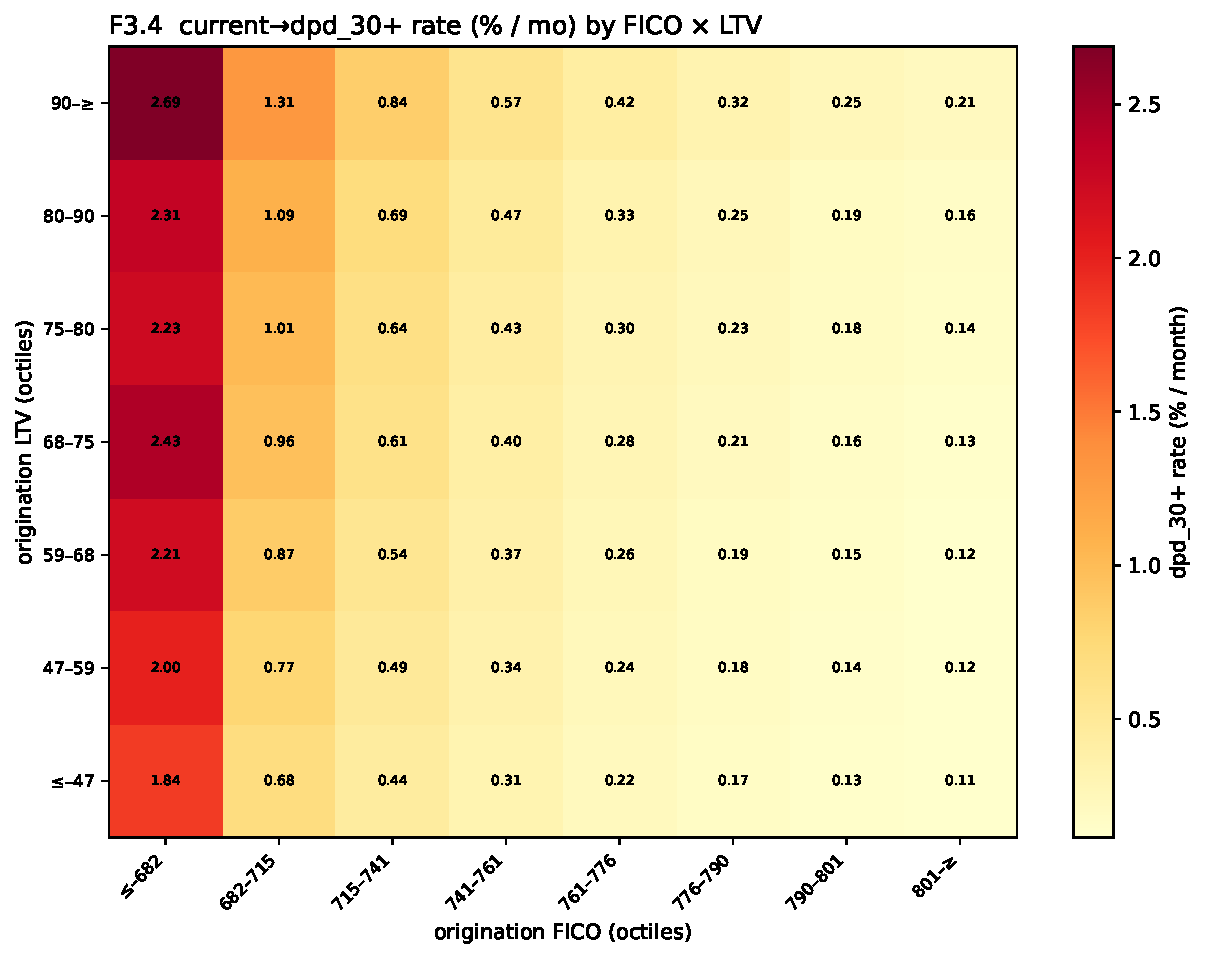
\includegraphics[width=0.78\textwidth]{figs/F3.4_fico_ltv_heatmap.pdf}
\caption[Monthly delinquency-entry rate on a credit-score $\times$ LTV
grid]{Monthly delinquency-entry rate on a credit-score $\times$ LTV grid
(equal-population bands): the additive credit-score gradient grows with
leverage --- additivity is misspecified.}\label{fig:interaction-ficoltv}
\end{figure}

\begin{figure}[htbp]\centering
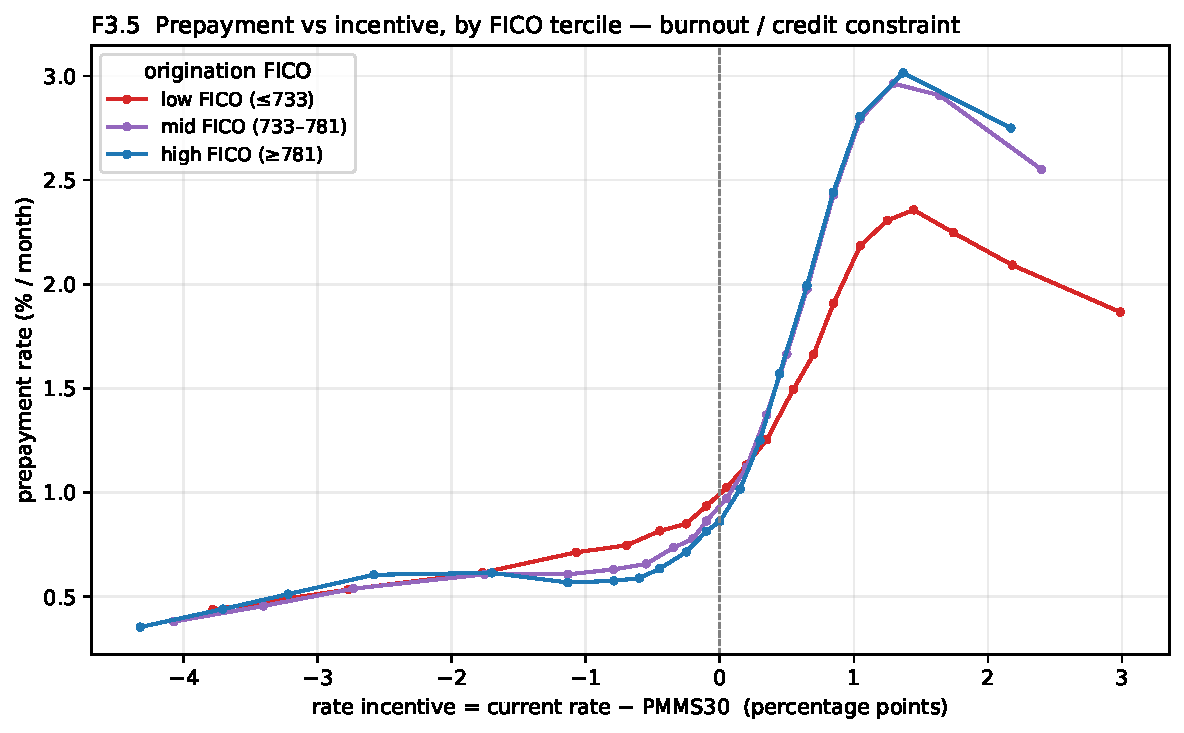
\includegraphics[width=0.8\textwidth]{figs/F3.5_incentive_fico.pdf}
\caption[The incentive S-curve by credit-score tercile]{The incentive
S-curve by credit-score tercile: the refinancing response to an
in-the-money option rises with credit
quality.}\label{fig:interaction-incfico}
\end{figure}

\begin{figure}[htbp]\centering
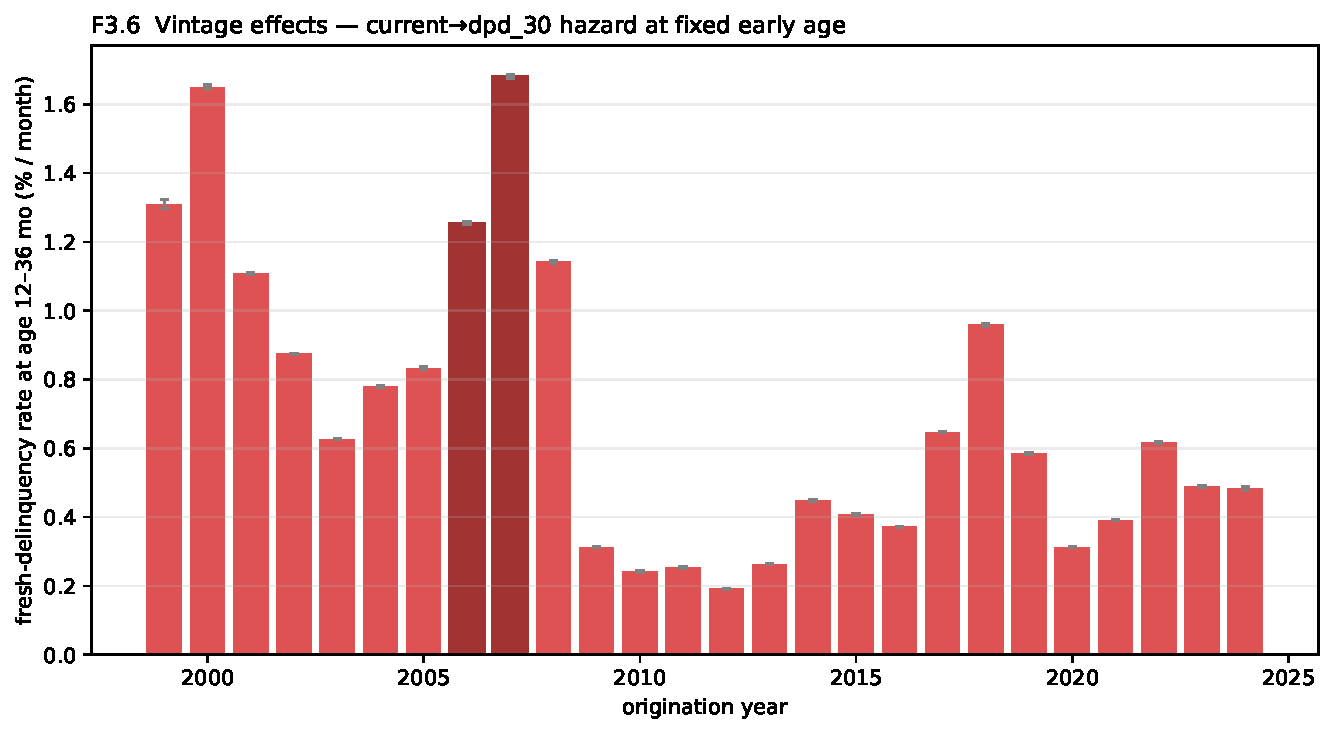
\includegraphics[width=0.8\textwidth]{figs/F3.6_vintage.pdf}
\caption[Delinquency hazard by origination cohort at fixed loan
age]{Delinquency hazard by origination cohort at fixed loan age
(12--36 months): the 2006--08 bubble vintages.}\label{fig:vintage}
\end{figure}

Taken together, the evidence points one way: monthly transition risk
depends on the covariates nonlinearly (the seasoning hump, the
incentive S-curve, convex credit-score decay) and interactively
(score$\times$leverage, incentive$\times$score, vintage).  A
linear-additive model should therefore underfit --- most severely on
prepayment, the channel combining the sharpest single-variable
nonlinearity with a first-order interaction --- and
Chapter~\ref{chap:results} tests precisely this.

% ────────────────────────────────────────────────────────────
\section{Comparison to Sirignano et al.\ (2021)}
\label{sec:data-comparison}

The dataset employed in the present study differs in several important
respects from the proprietary CoreLogic dataset used by
\citet{sirignano2021}, and these differences bear on the
interpretation of the results.

\citet{sirignano2021} draw on records for approximately 120 million
mortgages --- both prime and subprime --- originated across the United
States between January 1995 and June 2014, yielding approximately 3.5
billion loan-month observations.  The CoreLogic data encompass the
full spectrum of mortgage products, including fixed-rate,
adjustable-rate, hybrid, balloon, and interest-only loans, as well as
government-insured instruments.  Macro-economic covariates ---
zip-code-level house price indices from Zillow, county-level
unemployment rates from the Bureau of Labor Statistics, and the
Freddie Mac PMMS series --- are merged at the loan-month level within
the CoreLogic database.  The dataset is proprietary and cannot be
reproduced by independent researchers.

The Fannie Mae primary dataset, by contrast, is limited to
conventional fixed-rate fully-amortising loans and excludes both
subprime and government-insured products.  Macro-economic covariates
must be sourced and joined externally, as described in
Section~\ref{subsec:data-external}.  These differences have two
principal consequences.  First, the estimation sample is more
homogeneous in product mix; the nonlinear prepayment dynamics
associated with adjustable-rate burnout and subprime option exercise
--- prominent in \citeauthor{sirignano2021} --- are absent.  Second,
the absence of a subprime segment limits the range of credit-risk
outcomes observed; \citet{sirignano2021} report a median FICO score
of 630 for their subprime sub-sample against 730 for the prime
sub-sample, whereas the Fannie Mae population is concentrated at the
higher end of this credit-quality spectrum.

These limitations notwithstanding, the Fannie Mae dataset provides a
fully reproducible basis for the analysis.  The core methodological
contribution of \citet{sirignano2021} --- applying deep learning to a
multinomial competing-risks model of monthly loan-state transitions
--- transfers completely to the Fannie Mae panel.  The architecture,
estimation procedure, and evaluation framework described in subsequent
chapters are direct adaptations of that approach.  Table~\ref{tab:data-comparison}
summarises the key differences.

\begin{table}[htbp]
  \centering
  \small
  \begin{tabularx}{\textwidth}{@{} l X X @{}}
    \toprule
    \textbf{Dimension}
      & \textbf{Sirignano et al.\ (2021)}
      & \textbf{Present study} \\
    \midrule
    Data source
      & CoreLogic (proprietary)
      & Fannie Mae SFLP (public) \\[3pt]
    Total loans
      & ${\sim}120$ million
      & 57.6 million \\[3pt]
    Loan-month observations
      & ${\sim}3.5$ billion
      & 3.31 billion \\[3pt]
    Origination window
      & 1995--2014
      & 1999--2025 (full vintage set, reporting to 2025-12) \\[3pt]
    Products covered
      & Fixed, ARM, hybrid, balloon, IO
      & Fixed-rate, fully amortising only \\[3pt]
    Credit segments
      & Prime and subprime
      & Conventional (predominantly prime) \\[3pt]
    Macro covariates
      & Embedded (Zillow, BLS, PMMS)
      & External join required (FHFA HPI, PMMS) \\[3pt]
    Geographic detail
      & Full 5-digit zip code
      & 3-digit truncated zip; MSA \\[3pt]
    States modelled
      & Seven
      & Seven (identical mapping) \\[3pt]
    Reproducibility
      & Not publicly reproducible
      & Fully reproducible \\
    \bottomrule
  \end{tabularx}
  \caption[Comparison of the Fannie Mae SFLP dataset and the
  CoreLogic dataset used by Sirignano et al.\ (2021)]%
  {\textit{Comparison of the Fannie Mae SFLP primary dataset and the
  CoreLogic dataset used by \citet{sirignano2021}.}  CoreLogic counts
  are approximate as reported by the authors; Fannie Mae counts are
  measured on the assembled panel (Section~\ref{sec:data-summary}).}
  \label{tab:data-comparison}
\end{table}

%  to main.tex (after chapter2, before conclusions).
%
%  Required packages (add to the preamble of main.tex):
%      \usepackage{booktabs}
%      \usepackage{tabularx}
%      \usepackage{multirow}
%      \usepackage{natbib}   % or your preferred bib style
% ============================================================

\chapter{Data}
\label{chap:data}

% ────────────────────────────────────────────────────────────
\section{Data Source}
\label{sec:data-source}

This study employs the Fannie Mae Single-Family Loan Performance
(SFLP) dataset, a publicly available research dataset maintained by
the Federal National Mortgage Association (Fannie Mae) and updated on
a quarterly basis.  The dataset was originally released in April 2013
and contains origination and monthly performance records for a subset
of single-family conventional mortgage loans acquired by Fannie Mae
since January 2000.  New loan acquisitions and performance data are
added with an approximate four-month lag following the end of each
calendar quarter \citep{fanniemae2024}.

The data are organised as a \emph{loan-month panel}: each observation
corresponds to a single mortgage loan in a single monthly reporting
period, beginning at the month of acquisition and continuing until the
loan terminates through full prepayment, foreclosure, Real Estate
Owned (REO) disposition, or contractual maturity, or until the data
cut-off date.  This longitudinal structure is well-suited to the
competing-risks framing of \citet{sirignano2021}, which the present
study adapts to the Fannie Mae data.

Raw files are distributed as pipe-delimited CSV without a header row,
organised by acquisition quarter and identified by the convention
\texttt{YYYYQn.csv}.  Column identities are positional, fully
specified in the Fannie Mae Single-Family Loan Performance Data File
Layout and Glossary.  Each row contains 113 fields encoding static
origination attributes, dynamic monthly performance measures, and
post-termination expense and proceeds data.  The estimation sample
employed in this study is the \emph{complete} vintage set from a
single quarterly release: 104 acquisition-quarter files covering
cohorts from 2000Q1 onwards, with monthly reporting periods from
January 2000 through December 2025.  The assembled panel comprises
\textbf{3{,}312{,}456{,}883 loan-month observations across
57{,}562{,}668 loans} --- performance histories spanning four
interest-rate cycles, the 2008--11 foreclosure crisis, the COVID-era
forbearance episode, and the 2022--23 rate shock.

\subsection{From raw files to the estimation panel}
\label{subsec:data-pipeline}

Three distinct concepts in this dataset are colloquially called a
``quarter,'' and distinguishing them prevents the most common
assembly errors.  The \emph{acquisition vintage} identifies a file:
each \texttt{YYYYQn.csv} contains the loans Fannie Mae acquired in
that quarter, carrying their entire subsequent monthly history, and a
loan appears in exactly one file --- so concatenating all files
assembles the full sample with no duplication.  The \emph{monthly
reporting period} identifies a row, and this time dimension --- not
redundancy --- is why the dataset is large.  The \emph{release}
identifies the download: Fannie Mae republishes the entire dataset
quarterly with extended histories, so all files must come from one
release lest vintages carry inconsistent right-censoring dates; an
ingestion audit verifies a uniform cut-off across all 104 files.

Because no single file fits in memory ($\sim$800\,GB of raw CSV in
total), a six-stage pipeline converts the files into a compressed,
columnar store queried out of core: an integrity audit, streaming
conversion, type and sentinel cleaning, construction of the
transition panel with the outcome variable of
Section~\ref{sec:data-outcome}, sampling utilities, and a
reconciliation step that verifies row counts against the raw files.
Columnar storage means a query touching six of the 113 fields reads
roughly five per cent of the bytes, which is what makes the
full-panel descriptive statistics and exploratory analysis of
Sections~\ref{sec:data-summary} and~\ref{sec:data-eda}
computationally cheap.

% ────────────────────────────────────────────────────────────
\section{Population and Eligibility}
\label{sec:data-population}

The primary dataset is not a census of all loans in Fannie Mae's
guarantee book; it is a curated research sample subject to documented
eligibility and exclusion criteria \citep{fanniemae2024}.  The
population is restricted to fixed-rate, fully amortising,
full-documentation single-family conventional mortgage loans with
original terms of at least five years and less than 35 years,
originated on or after 1 January 1999 and acquired by Fannie Mae on
or after 1 January 2000.

A number of product types are explicitly excluded.  Adjustable-rate
mortgages, interest-only loans, balloon-amortisation mortgages, and
loans carrying prepayment penalties are absent from the dataset.
Also excluded are loans with original loan-to-value (LTV) ratios
exceeding 97 per cent, Alt-A and other reduced-documentation
products, government-insured loans (FHA and VA), loans subject to
long-term standby commitments or third-party risk-sharing
arrangements other than primary mortgage insurance, and loans
acquired on a negotiated bulk basis.  Loans with non-standard payment
due dates and loans that liquidated in the same month as acquisition
are similarly excluded.  Fannie Mae's Home Affordable Refinance
Program (HARP) loans are likewise absent from the primary dataset;
when a loan in the primary dataset was subsequently refinanced through
HARP, its termination is recorded as a standard prepayment, and its
post-refinance performance is not tracked here.  This is discussed
further in Section~\ref{sec:data-outcome}.

These restrictions yield a sample of conventionally underwritten
fixed-rate mortgages broadly representative of the agency conventional
loan market under post-crisis underwriting standards.  The exclusion
of adjustable-rate and interest-only products limits the range of
prepayment incentive dynamics captured relative to the full-spectrum
dataset used by \citet{sirignano2021}; this is discussed in
Section~\ref{sec:data-comparison}.  Table~\ref{tab:eligibility}
summarises the principal eligibility criteria and exclusions.

\begin{table}[htbp]
  \centering
  \small
  \begin{tabularx}{\textwidth}{@{} l X @{}}
    \toprule
    \textbf{Criterion} & \textbf{Requirement / Exclusion} \\
    \midrule
    Origination date      & On or after 1 January 1999 \\[2pt]
    Acquisition date      & On or after 1 January 2000 \\[2pt]
    Product type          & Fixed-rate, fully amortising only \\[2pt]
    Loan term             & $5 \leq \mathrm{term} < 35$ years at origination \\[2pt]
    Documentation         & Full documentation only \\[2pt]
    LTV at origination    & $\leq 97\%$ \\[4pt]
    \emph{Excluded: product}      & ARM, interest-only, balloon,
                                    prepayment-penalty loans \\[2pt]
    \emph{Excluded: credit class} & Alt-A, reduced-documentation,
                                    streamlined processing \\[2pt]
    \emph{Excluded: guarantee}    & Government-insured (FHA, VA) loans \\[2pt]
    \emph{Excluded: structure}    & Long-term standby commitments;
                                    bulk acquisitions; lender-recourse
                                    loans (except primary MI) \\[2pt]
    \emph{Excluded: programme}    & HARP and Refi Plus loans \\[2pt]
    \emph{Excluded: payment}      & Bi-weekly and non-first-of-month
                                    due dates \\[2pt]
    \emph{Excluded: timing}       & Loans liquidated in month of
                                    acquisition \\
    \bottomrule
  \end{tabularx}
  \caption[Eligibility criteria for the Fannie Mae SFLP primary dataset]%
  {\textit{Eligibility criteria for the Fannie Mae SFLP primary
  dataset.}  Source: Fannie Mae Single-Family Loan Performance
  Dataset FAQs \citep{fanniemae2024}.}
  \label{tab:eligibility}
\end{table}

% ────────────────────────────────────────────────────────────
\section{Variables}
\label{sec:data-variables}

The 113 fields in each monthly observation can be organised into three
functional groups: static origination attributes, dynamic monthly
performance attributes, and post-termination resolution data.  The
model uses a subset of these fields as covariates.  Two fields --- the
Current Loan Delinquency Status and the Zero Balance Code --- serve as
the primary inputs from which the outcome variable is constructed.

% ────────────────────────────────
\subsection{Origination Attributes}
\label{subsec:data-origination}

Static origination attributes are recorded at loan delivery and do
not change over the life of the loan absent a modification.  The
borrower's FICO credit score at origination is available for both the
primary borrower and, where applicable, a co-borrower; prior to the
January 2015 dataset release only the lower of the two scores was
disclosed, and a missingness indicator is constructed accordingly.
Continuous origination covariates include the original
debt-to-income (DTI) ratio, original LTV ratio, original combined LTV
(CLTV, which incorporates subordinate liens), original unpaid
principal balance (UPB), original interest rate, and original loan
term in months.  Categorical origination attributes include the
acquisition channel (retail, broker, or correspondent), loan purpose
(purchase, rate-term refinance, or cash-out refinance), property type,
occupancy status (primary residence, second home, or investment
property), property state, Metropolitan Statistical Area (MSA), and
three-digit truncated zip code.  The truncation of the zip code
reflects borrower privacy considerations; full zip codes are not
disclosed in the dataset \citep{fanniemae2024}.

% ────────────────────────────────
\subsection{Dynamic Performance Attributes}
\label{subsec:data-performance}

Dynamic performance attributes are updated in each monthly reporting
period.  The current actual unpaid principal balance reflects the
outstanding loan balance at each point in time.  Loan age, measured
in months from the first payment date, and the remaining months to
legal maturity are derived from the contractual amortisation schedule.
The current interest rate reflects the applicable note rate, updated
when a modification changes the loan terms.

Two dynamic fields jointly determine the outcome variable.  The
\textbf{Current Loan Delinquency Status} reports the number of missed
monthly payments as a two-character code: \texttt{00} denotes a
current loan; \texttt{01}, \texttt{02}, and codes \texttt{03} and
above denote 30-, 60-, and 90-or-more-day delinquencies respectively;
and \texttt{XX} denotes an unavailable status.  The \textbf{Zero
Balance Code} is populated exclusively in the terminal monthly
observation and classifies the manner of loan termination into nine
categories, distinguishing between voluntary prepayments, third-party
foreclosure sales, short sales, repurchases, REO dispositions, note
sales, and non-credit removals.  (The dataset also carries a 24-month
payment-history string; it is not used as a model input here, since
the current state and loan-level covariates already summarise the
information the transition model conditions on.)

% ────────────────────────────────
\subsection{Externally Sourced Covariates}
\label{subsec:data-external}

A small, fixed set of external macroeconomic series is joined to the
loan-level panel at feature-construction time (the stored panel
itself is never rewritten); Table~\ref{tab:macrovars} summarises the
sources.  The Freddie Mac Primary Mortgage Market Survey (PMMS)
weekly fixed-rate series, aggregated to calendar-month means, supplies
the prevailing market mortgage rate from which the \emph{rate
incentive} of Equation~\eqref{eq:incentive} is computed --- the
refinancing option value, the primary driver of prepayment behaviour
in the empirical mortgage literature
\citep{schwartz1989,sirignano2021}.  Unemployment rates enter at both
national (Bureau of Labor Statistics) and state level, the latter
because the cross-sectional dispersion in labour-market conditions
(Nevada versus Texas in 2009) is precisely the variation a national
series cannot supply.  House prices enter through the Freddie Mac
House Price Index at national and state level, from which the
mark-to-market loan-to-value ratio of Equation~\eqref{eq:mtmltv} ---
the principal determinant of the default option value
\citep{deng2000} --- and the trailing twelve-month house-price change
are constructed.  The ten-year Treasury yield completes the set.

Each series is joined with a \emph{publication lag} reflecting when
the value was actually observable: rates are published in real time
(no lag), month-$t$ unemployment is released early in month $t{+}1$
(one-month lag), and the house-price index roughly two months after
the reference month (two-month lag).  Final-revision series are used
rather than real-time vintages --- a stated limitation, standard for
historical studies.  Where a state-level value is unavailable
(territories; series start dates) the national value substitutes,
with an indicator flag carried as a model feature.

\begin{table}[htbp]
  \centering
  \small
  \begin{tabularx}{\textwidth}{@{} l l l l c @{}}
    \toprule
    \textbf{Variable} & \textbf{Source} & \textbf{Geography}
      & \textbf{Monthly value} & \textbf{Lag} \\
    \midrule
    30-yr mortgage rate & Freddie Mac PMMS & national & month mean & 0\,m \\
    10-yr Treasury yield & FRED \texttt{DGS10} & national & month mean & 0\,m \\
    Unemployment rate & BLS (via FRED) & national + state & as published & 1\,m \\
    House-price index & Freddie Mac FMHPI & national + state & as published & 2\,m \\
    \bottomrule
  \end{tabularx}
  \caption[External macroeconomic covariates and join conventions]%
  {\textit{External macroeconomic covariates and join conventions.}
  A loan-month at calendar month $t$ is joined to the macro value of
  month $t-\ell$, where $\ell$ is the publication lag.  Seasonally
  adjusted versions are used throughout.}
  \label{tab:macrovars}
\end{table}

As a check on the incentive variable, a market-rate proxy derived
from the panel itself --- the average note rate of loans originated
in each calendar month --- tracks the PMMS series with correlation
$0.991$, root-mean-square deviation $0.198$ percentage points, and
mean absolute deviation $0.147$ percentage points, with a mean gap of
essentially zero.  The PMMS-based incentive is the primary feature;
the panel-derived proxy is retained as a robustness alternative,
demonstrating that the incentive variable is not an artefact of one
data source.

% ────────────────────────────────────────────────────────────
\section{Outcome Variable}
\label{sec:data-outcome}

Following \citet{sirignano2021}, the outcome variable is a categorical
measure of mortgage state in month $t+1$, conditional on the loan's
state and covariate vector in month $t$.  Seven mutually exclusive
states are defined: \emph{Current}, \emph{30 Days Past Due}
(30\,DPD), \emph{60 Days Past Due} (60\,DPD), \emph{90+ Days Past
Due} (90+\,DPD), \emph{Foreclosure}, \emph{Real Estate Owned} (REO),
and \emph{Prepaid}.

State assignment for each loan-month observation follows a
deterministic hierarchy.  When the Zero Balance Code is present ---
indicating the terminal observation for the loan --- the termination
type is mapped to the Foreclosure, REO, or Prepaid absorbing state as
shown in Table~\ref{tab:state-mapping}.  When the Zero Balance Code is
absent, the delinquency status field governs: codes \texttt{00}
through \texttt{03} and above map to Current, 30\,DPD, 60\,DPD, and
90+\,DPD respectively, while \texttt{XX} is treated as missing.  The
state in month $t+1$ is obtained by a window lead over the reporting
period dimension, partitioned by loan identifier.  Loans whose final
observation falls at or before the data cut-off without a recorded
termination event receive a censored indicator and are excluded from
the labelled target.

Regarding HARP loans: as noted in Section~\ref{sec:data-population},
any loan in the primary dataset that was refinanced through the
HARP programme terminates with a Zero Balance Code of \texttt{01}
(prepaid) at the moment of refinancing and is therefore treated as a
standard prepayment in the outcome variable.  This approximation is
defensible given that the loan is extinguished from Fannie Mae's
credit exposure in either case, though it may marginally overstate
the rate-incentive sensitivity of the prepayment hazard during the
period of peak HARP activity (approximately 2009--2013).

\begin{table}[htbp]
  \centering
  \small
  \begin{tabularx}{\textwidth}{@{} l l l X @{}}
    \toprule
    \textbf{State} & \textbf{Source field} & \textbf{Condition}
      & \textbf{Economic interpretation} \\
    \midrule
    Current
      & Delinquency Status & \texttt{= 00}
      & Borrower is contractually current on all payments. \\[3pt]
    30\,DPD
      & Delinquency Status & \texttt{= 01}
      & One missed monthly payment. \\[3pt]
    60\,DPD
      & Delinquency Status & \texttt{= 02}
      & Two consecutive missed monthly payments. \\[3pt]
    90+\,DPD
      & Delinquency Status & \texttt{$\geq$ 03}
      & Three or more missed payments; serious delinquency. \\[3pt]
    Foreclosure
      & Zero Balance Code  & \texttt{02, 03, 15,}
      & Credit-loss termination: third-party sale, short sale, \\
      &                    & \texttt{97, 98}
      & note sale, or credit-event repurchase. \\[3pt]
    REO
      & Zero Balance Code  & \texttt{= 09}
      & Fannie Mae acquires ownership of the property. \\[3pt]
    Prepaid
      & Zero Balance Code  & \texttt{01, 06, 16,}
      & Full payoff, contractual maturity, repurchase, \\
      &                    & \texttt{96}
      & or non-credit removal (including HARP exits). \\
    \bottomrule
  \end{tabularx}
  \caption[Mapping of Fannie Mae data fields to the seven-state
  outcome variable]%
  {\textit{Mapping of Fannie Mae data fields to the seven-state
  outcome variable.}  The Zero Balance Code is populated only in the
  terminal monthly observation; the Delinquency Status governs state
  assignment in all non-terminal periods.}
  \label{tab:state-mapping}
\end{table}

One structural feature of this dataset deserves emphasis: because the
Foreclosure, REO, and Prepaid states are derived from the Zero
Balance Code --- populated only in a loan's final observation ---
these three states are \emph{absorbing}.  There is no ongoing ``in
foreclosure'' monthly status as in the CoreLogic data of
\citet{sirignano2021}, where loans in formal foreclosure are observed
month by month and occasionally return to performing status.  The
origin set here therefore comprises the four live states (Current
through 90+\,DPD) while destinations span all seven: the transition
matrix is $4\times 7$ rather than $7\times 7$
(Section~\ref{sec:meth-model}).  Within the live states the data are
rich in both directions --- delinquency deepens at most one bucket
per month, but cures can jump multiple buckets, and a meaningful
fraction of seriously delinquent loans return to current.  The
seven-state formulation captures this in a way that a binary
default-versus-prepayment classification would obscure, and the
empirical monthly transition matrix derived from each training window
serves as the floor benchmark for the model comparison
(Section~\ref{subsec:meth-empirical}).

% ────────────────────────────────────────────────────────────
\section{Panel Composition and Summary Statistics}
\label{sec:data-summary}

The assembled panel comprises 3{,}312{,}456{,}883 loan-month
observations across 57{,}562{,}668 loans in 104 acquisition-vintage
partitions, with reporting months from January 2000 through December
2025.  Table~\ref{tab:stateshares} reports the distribution of
loan-months across the seven states.  Two features dominate.  First,
extreme class imbalance: the Current state accounts for $96.28\%$ of
all loan-months, while the credit-event terminals occur at roughly
one in ten thousand observations --- the empirical fact behind both
the importance-weighted thinning of training data
(Section~\ref{sec:meth-design}) and the Laplace smoothing of the
empirical benchmark (Section~\ref{subsec:meth-empirical}).  Second,
the rare states are nonetheless abundantly populated in absolute
terms (REO alone contributes roughly half a million loan-months),
which is what permits stable estimation of rare-transition
probabilities at this scale.

\begin{table}[htbp]
  \centering
  \small
  \begin{tabular}{l r @{\qquad\qquad} l r}
    \toprule
    \textbf{State} & \textbf{Share} & \textbf{State} & \textbf{Share} \\
    \midrule
    Current  & 96.28\,\% & 60\,DPD     & 0.31\,\%   \\
    Prepaid  & 1.25\,\%  & REO         & 0.014\,\%  \\
    30\,DPD  & 1.15\,\%  & Foreclosure & 0.0067\,\% \\
    90+\,DPD & 0.98\,\%  &             &            \\
    \bottomrule
  \end{tabular}
  \caption[Distribution of loan-months across the seven states]%
  {\textit{Distribution of loan-months across the seven states},
  full panel, 2000--2025 (3.31 billion loan-months).}
  \label{tab:stateshares}
\end{table}

Pooled over time, the monthly transition rates out of Current are
$1.27\%$ to Prepaid and $0.64\%$ to 30\,DPD.  The pooling, however,
hides the economics: Figure~\ref{fig:transitionrates} plots the
monthly series over 2000--2025, displaying the 2003 and 2020--21
refinancing waves in the prepayment rate, the 2008--11 default wave
in the delinquency rates, and the sharp 2022--23 collapse in
prepayments as market rates rose.  These regime shifts --- rather
than any single structural break --- are the empirical justification
for the rolling backtest design of Section~\ref{sec:meth-design}.
During 2020--21 the delinquency-status codes additionally reflect
COVID-era forbearance, which manifests as unusual persistence in
delinquency states followed by elevated cure rates; no special
treatment is applied, but results involving those years are read with
this in mind.

\begin{figure}[htbp]\centering
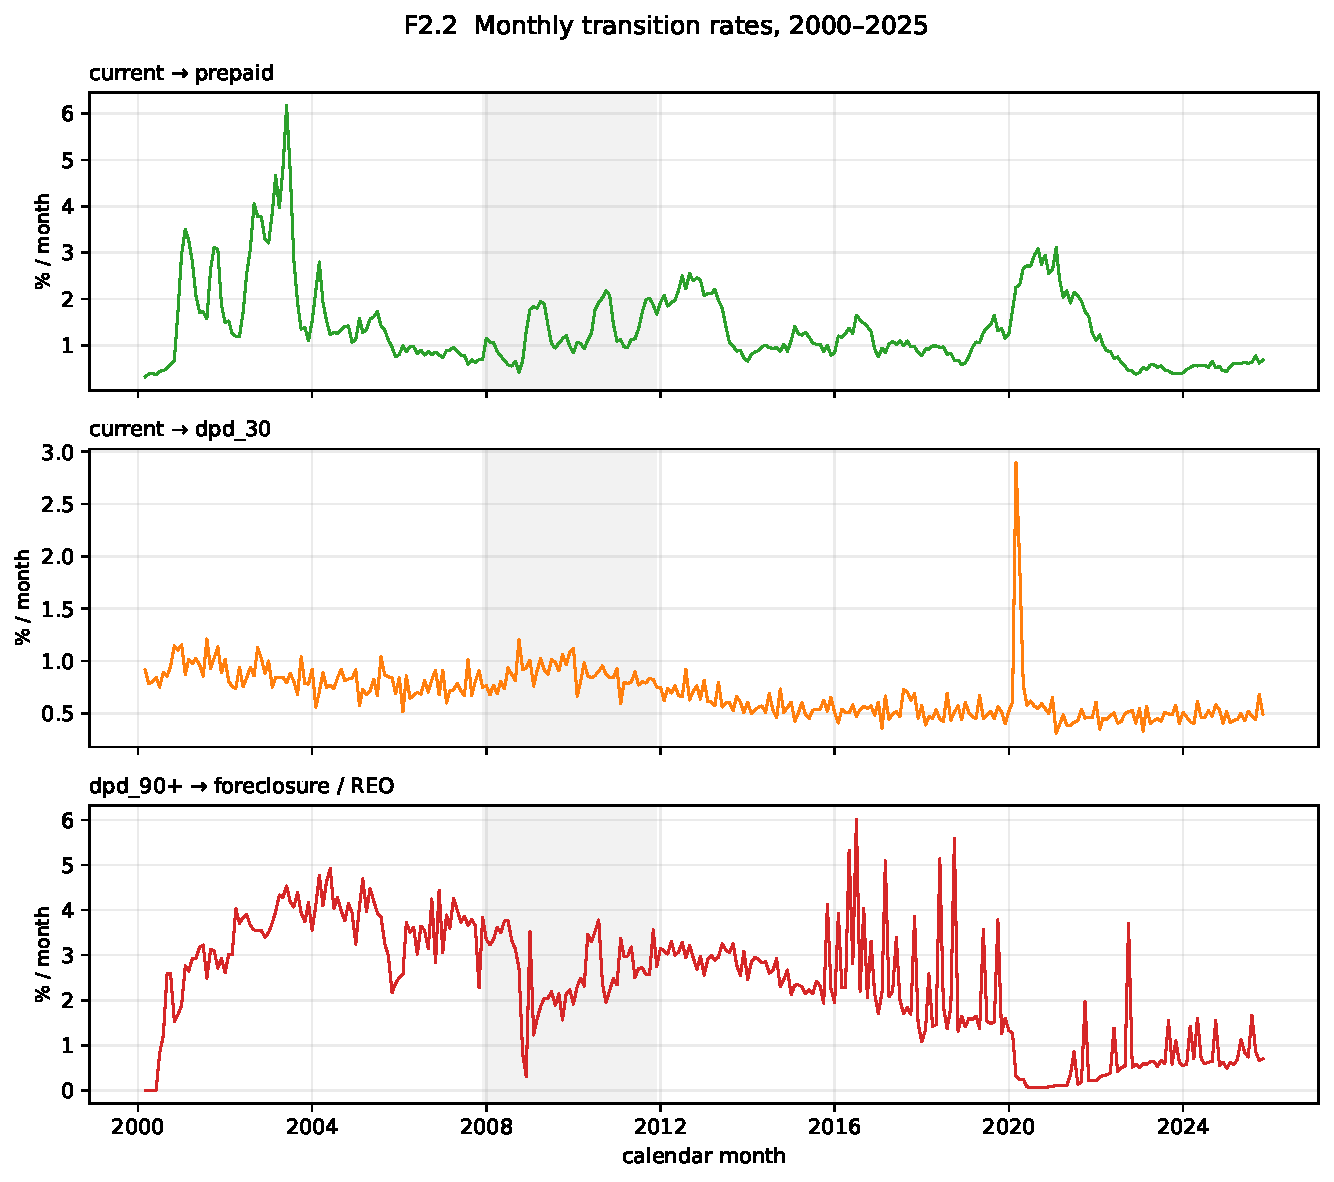
\includegraphics[width=0.9\textwidth]{figs/F2.2_transition_rates.pdf}
\caption[Monthly transition rates out of the Current state]{Monthly
transition rates out of the Current state, 2000--2025: prepayment and
entry into 30\,DPD (left axis), serious-delinquency terminations
(right axis).  Vertical shading marks the 2008--11 crisis and the
2020--21 forbearance episode.}\label{fig:transitionrates}
\end{figure}

\begin{table}[htbp]\centering\small
\caption[Summary statistics of model covariates]{Summary statistics of
the continuous model covariates over the full panel: null rate, mean,
standard deviation, and the min/1st/25th/50th/75th/99th/max
percentiles.}\label{tab:covariate-summary}
\resizebox{\textwidth}{!}{% Source: outputs/tables/eda/T1.2_covariate_summary_continuous.tex (full-panel
% Stage-6 QA). Tabular-only; wrap in \resizebox in chapter3.tex. Caption+label there.
\begin{tabular}{lrrrrrrrrrrl}
\toprule
column & null\_rate & mean & std & min & p01 & p25 & median & p75 & p99 & max & log\_flagged \\
\midrule
Original Interest Rate & 0 & 4.71882 & 1.32648 & 1.5 & 2.36602 & 3.62711 & 4.62688 & 5.75 & 7.85794 & 16.5 & False \\
Current Interest Rate & 0.012707 & 4.68763 & 1.32523 & 0 & 2.28982 & 3.625 & 4.60188 & 5.75 & 7.83746 & 13.5 & False \\
Original UPB & 0 & 199755 & 121639 & 1000 & 38809.4 & 109817 & 170562 & 262260 & 596156 & 2.326e+06 & True \\
Current Actual UPB & 0 & 159715 & 124113 & 0 & 0 & 71875.9 & 134287 & 224204 & 564970 & 2.86e+06 & True \\
Original Loan Term & 0 & 306.643 & 82.0617 & 36 & 120 & 202.959 & 360 & 360 & 360 & 360 & False \\
Loan Age & 0.01272 & 46.8107 & 42.4782 & -3 & 0 & 15 & 34.9747 & 65.8525 & 188.817 & 322 & False \\
Remaining Months to Maturity & 0.027474 & 252.795 & 97.4912 & 0 & 22.5446 & 167.472 & 294.279 & 335.84 & 359 & 480 & False \\
Original Loan-to-Value (LTV) & 0 & 69.7447 & 17.8489 & 1 & 21.1656 & 59.0522 & 74.5451 & 80 & 97 & 105 & False \\
Original Combined LTV (CLTV) & 0.003362 & 70.4277 & 17.9251 & 1 & 21.6837 & 59.7414 & 75 & 80 & 97 & 199 & False \\
Debt-to-Income (DTI) & 0.014108 & 33.3364 & 11.2275 & 0 & 9.02377 & 25 & 33.6755 & 41.9385 & 60.056 & 64 & False \\
fico\_orig & 0.002844 & 746.693 & 52.418 & 300 & 603.635 & 712.774 & 759.539 & 788.96 & 817.552 & 850 & False \\
fico\_co & 0.515382 & 754.702 & 49.6835 & 300 & 611.863 & 725.849 & 768.606 & 793.443 & 818.68 & 850 & False \\
Mortgage Insurance Percentage & 0.810875 & 24.1429 & 7.26184 & 0.12 & 6 & 22.29 & 25 & 30 & 35 & 50 & False \\
Number of Borrowers & 0.000119 & 1.55013 & 0.514524 & 1 & 1 & 1 & 2 & 2 & 2 & 10 & False \\
Number of Units & 0 & 1.03643 & 0.248099 & 1 & 1 & 1 & 1 & 1 & 2 & 4 & False \\
\bottomrule
\end{tabular}
}
\end{table}

% ────────────────────────────────────────────────────────────
\section{Exploratory Evidence: Nonlinearity and Interactions}
\label{sec:data-eda}

Before any model is fitted, the case that nonlinear modelling is
\emph{needed} can be made by counting alone.  The instrument is the
empirical hazard curve: bucket a covariate into equal-population
bins and plot the realised one-month transition rate per bin, with
Wilson 95\% confidence intervals.  Because each curve is a single
out-of-core aggregation over the columnar panel, the entire
programme runs in minutes.

\subsection{Single-covariate nonlinearity}
\label{subsec:data-eda-single}

Three hazard curves carry the argument.
\emph{Prepayment versus loan age}
(Figure~\ref{fig:hazard-age}): the rate rises from $0.27\%$ per month
at origination to a peak of $1.56\%$ at approximately 17 months of
age, then decays to $1.11\%$ by month 52 --- the classic
``seasoning hump,'' strongly non-monotone, with a secondary late-life
rise among long-surviving loans.  \emph{Prepayment versus the
refinancing incentive} (Figure~\ref{fig:hazard-incentive}): the rate
is flat at $0.4$--$0.6\%$ per month while the option is out of the
money, turns up sharply through zero, peaks at $2.71\%$ near
$+1.5$ percentage points of incentive, and falls back to $2.16\%$ by
$+2.7$ --- a roughly sevenfold range containing both an inflection
and a turning point, reproducing the flagship nonlinearity of
\citet{sirignano2021} on this cleaner credit box.
\emph{Delinquency versus credit score}
(Figure~\ref{fig:hazard-fico}): the entry rate into 30\,DPD falls
twenty-four-fold, from $3.06\%$ per month at FICO ${\approx}623$ to
$0.13\%$ at FICO ${\approx}815$, and the decay is convex --- the
slope in the low-score half is roughly $3.7$ times that in the
high-score half.  None of the three shapes is representable by a
linear term.

\begin{figure}[htbp]\centering
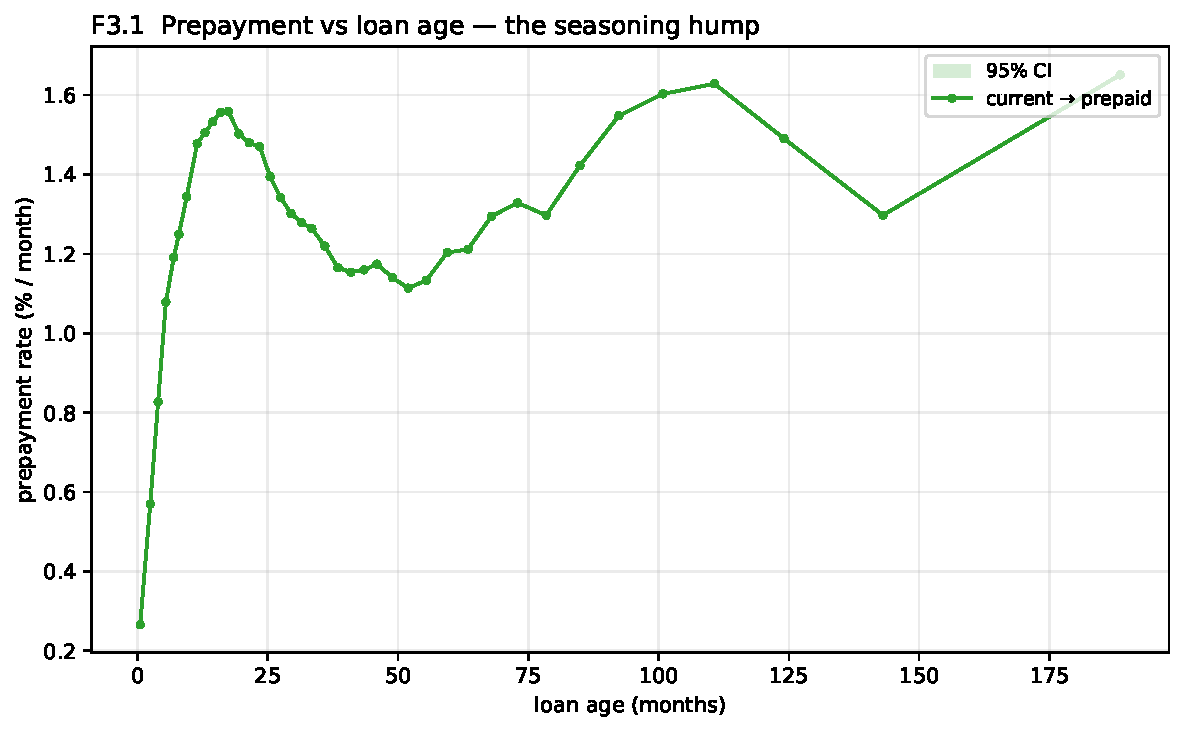
\includegraphics[width=0.8\textwidth]{figs/F3.1_prepay_age.pdf}
\caption[Empirical prepayment hazard by loan age]{Empirical prepayment
hazard by loan age (equal-population buckets, Wilson 95\% intervals):
the seasoning hump.}\label{fig:hazard-age}
\end{figure}

\begin{figure}[htbp]\centering
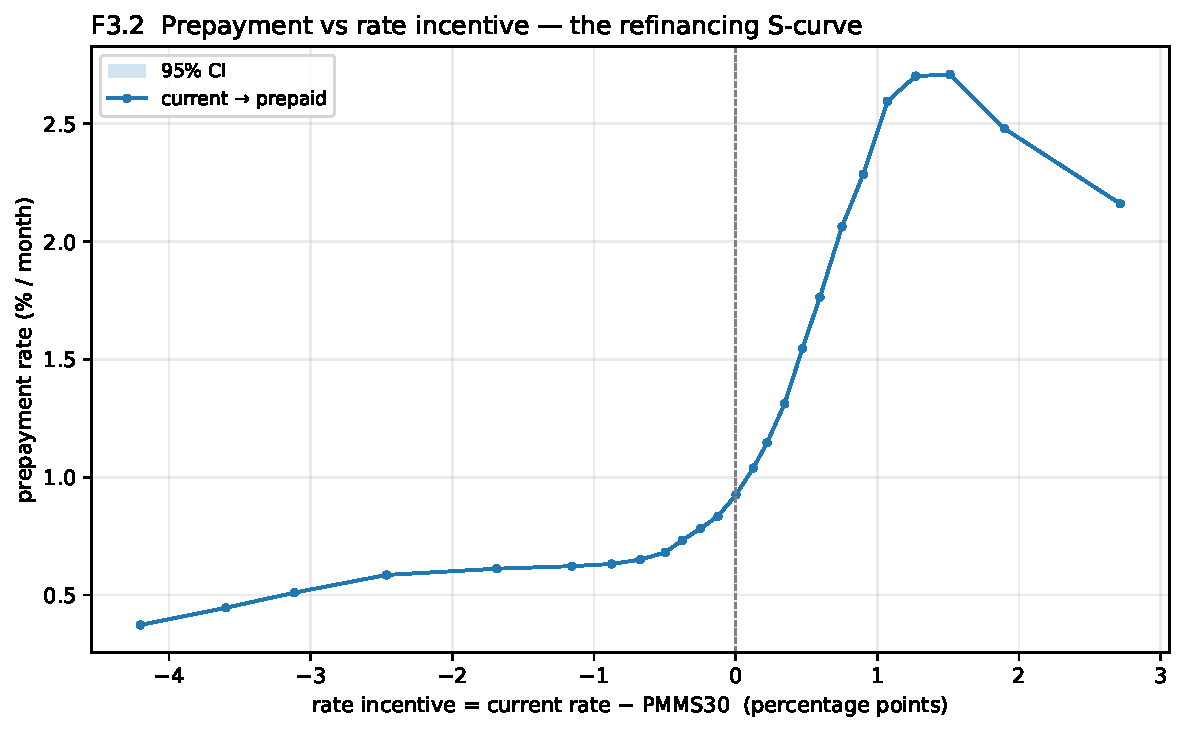
\includegraphics[width=0.8\textwidth]{figs/F3.2_prepay_incentive.pdf}
\caption[Empirical prepayment hazard by refinancing incentive]{Empirical
prepayment hazard by refinancing incentive: the S-curve, with burnout
beyond $+1.5$\,pp.}\label{fig:hazard-incentive}
\end{figure}

\begin{figure}[htbp]\centering
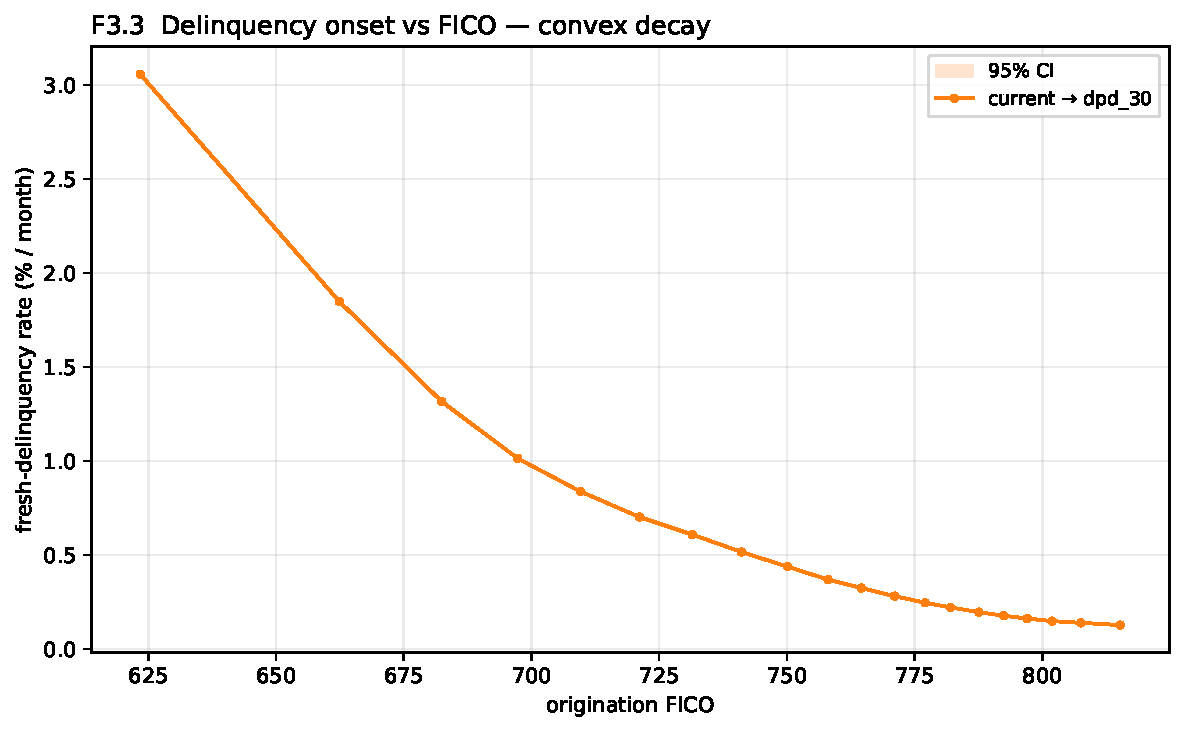
\includegraphics[width=0.8\textwidth]{figs/F3.3_delinq_fico.pdf}
\caption[Empirical 30\,DPD entry hazard by origination credit
score]{Empirical 30\,DPD entry hazard by origination credit score:
convex decay.}\label{fig:hazard-fico}
\end{figure}

\subsection{Interactions: the case against additivity}
\label{subsec:data-eda-interactions}

A linear-\emph{additive} model could in principle be patched with
transformed single-variable terms; interactions are what it cannot
absorb.  On a credit-score~$\times$~LTV grid
(Figure~\ref{fig:interaction-ficoltv}), the monthly rate of entry
into delinquency ranges from $0.11\%$ (best scores, lowest leverage)
to $2.69\%$ (worst scores, highest leverage) --- and decisively, the
\emph{additive} credit-score gradient (worst-minus-best rate) grows
from $1.73$ percentage points at low LTV to $2.48$ at high LTV, a
$43\%$ increase; equivalently, the leverage effect is roughly
$8.5$ times larger for low-score than high-score borrowers.
Additivity forces this gradient to be constant; the violation sits
exactly in the low-score/high-leverage corner that drives credit
losses.  In the prepayment channel
(Figure~\ref{fig:interaction-incfico}), splitting the incentive
S-curve by credit-score tercile shows the in-the-money refinancing
response \emph{rising} with credit quality --- $2.36\%$ per month in
the lowest tercile against $3.01\%$ in the highest --- because
credit-constrained borrowers cannot exercise the option: the
incentive \emph{slope} itself depends on the score.  Finally, holding
loan age fixed at 12--36 months to strip out seasoning, the
delinquency hazard by origination cohort isolates a clean vintage
effect: the 2007 cohort peaks at $1.68\%$ per month against $0.47\%$
for calm cohorts --- a $3.6$-fold premium
(Figure~\ref{fig:vintage}) --- so the origination vintage is a
feature in its own right, not reducible to contemporaneous
covariates.

\begin{figure}[htbp]\centering
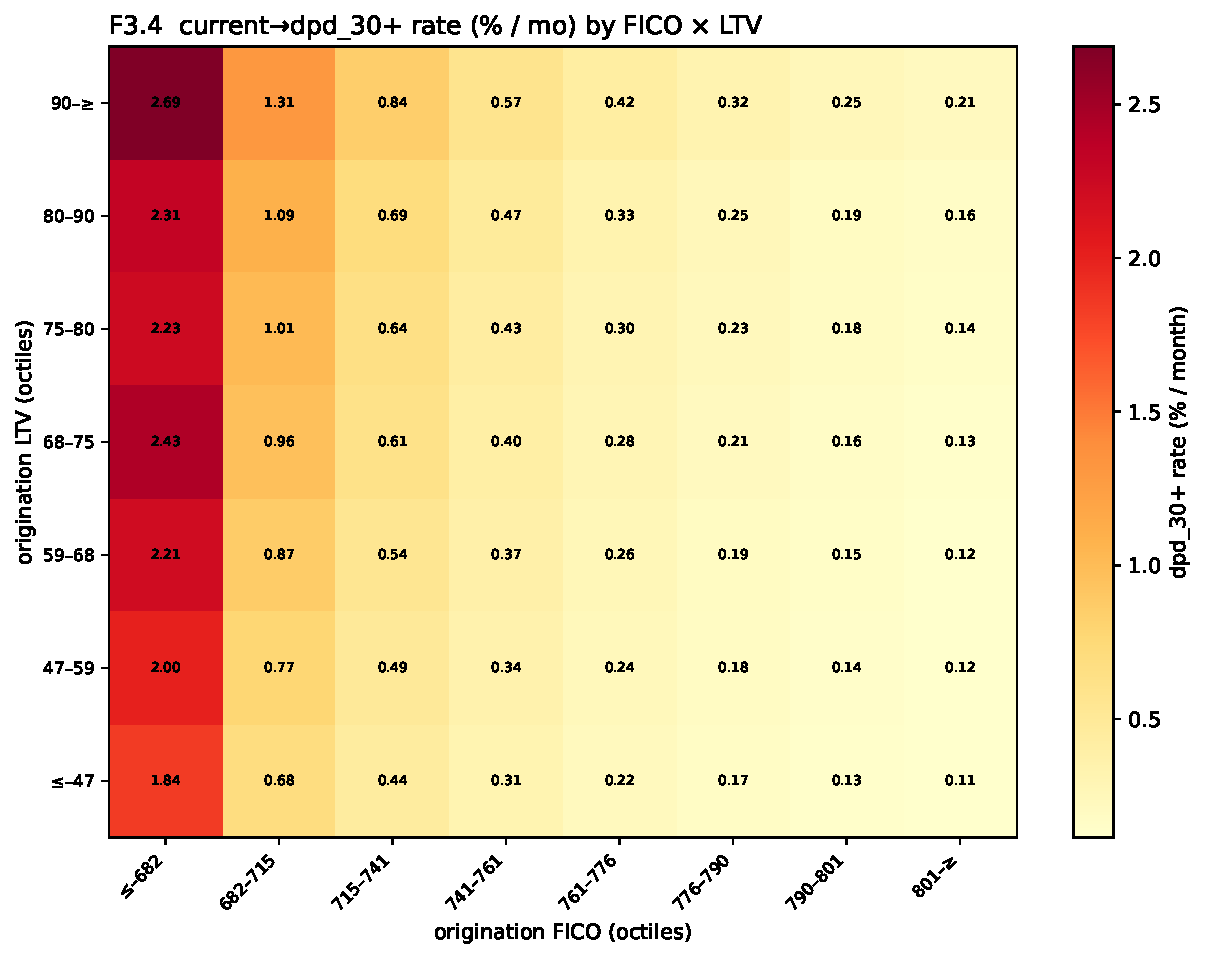
\includegraphics[width=0.78\textwidth]{figs/F3.4_fico_ltv_heatmap.pdf}
\caption[Monthly delinquency-entry rate on a credit-score $\times$ LTV
grid]{Monthly delinquency-entry rate on a credit-score $\times$ LTV grid
(equal-population bands): the additive credit-score gradient grows with
leverage --- additivity is misspecified.}\label{fig:interaction-ficoltv}
\end{figure}

\begin{figure}[htbp]\centering
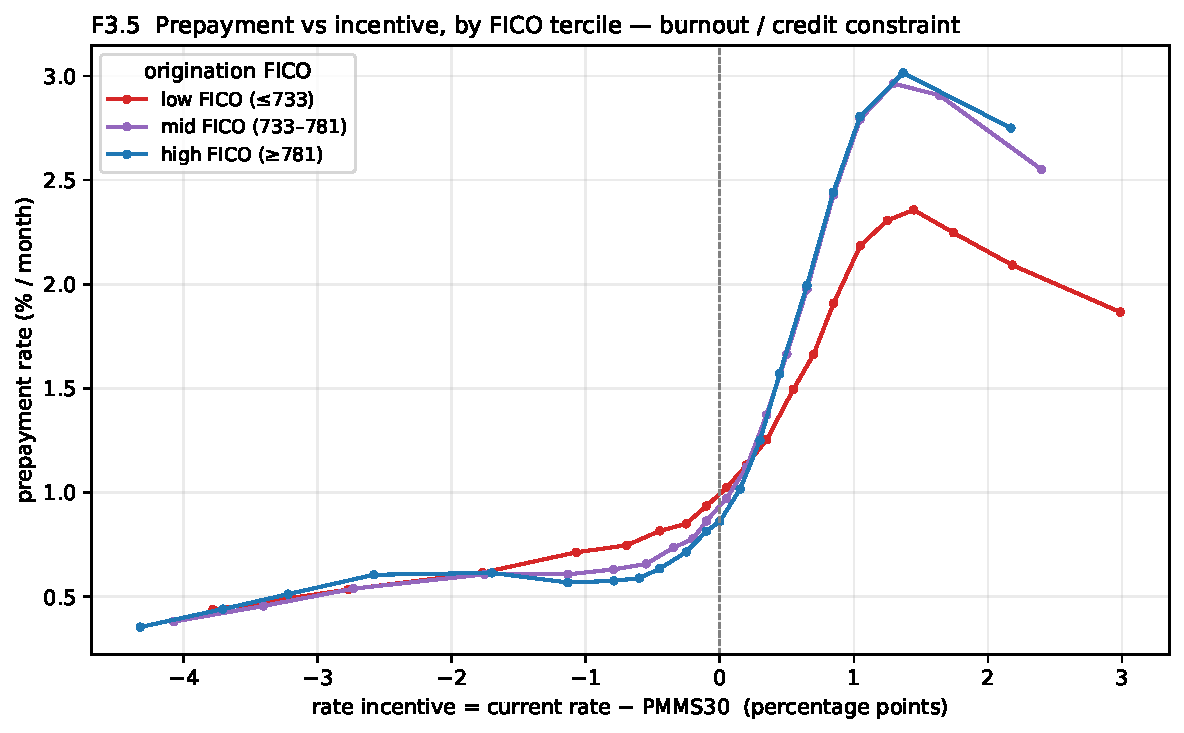
\includegraphics[width=0.8\textwidth]{figs/F3.5_incentive_fico.pdf}
\caption[The incentive S-curve by credit-score tercile]{The incentive
S-curve by credit-score tercile: the refinancing response to an
in-the-money option rises with credit
quality.}\label{fig:interaction-incfico}
\end{figure}

\begin{figure}[htbp]\centering
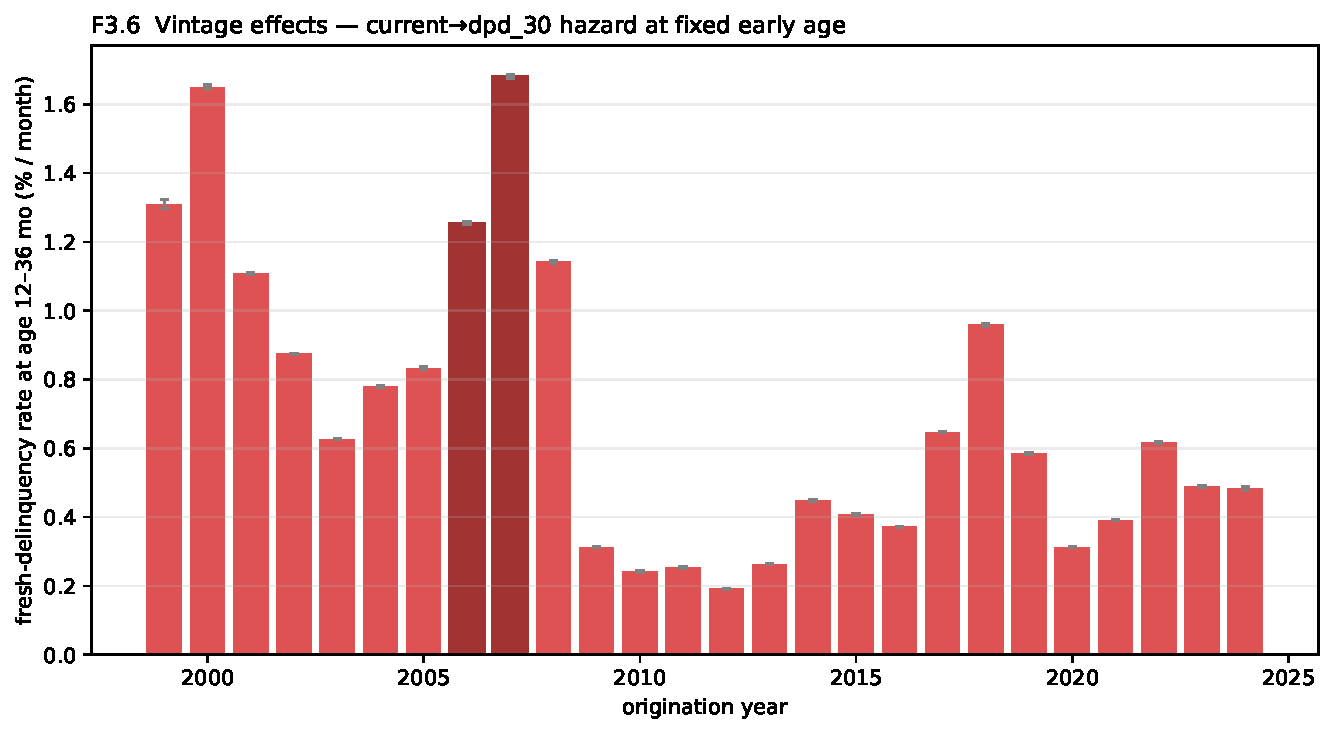
\includegraphics[width=0.8\textwidth]{figs/F3.6_vintage.pdf}
\caption[Delinquency hazard by origination cohort at fixed loan
age]{Delinquency hazard by origination cohort at fixed loan age
(12--36 months): the 2006--08 bubble vintages.}\label{fig:vintage}
\end{figure}

Taken together, the evidence points one way: monthly transition risk
depends on the covariates nonlinearly (the seasoning hump, the
incentive S-curve, convex credit-score decay) and interactively
(score$\times$leverage, incentive$\times$score, vintage).  A
linear-additive model should therefore underfit --- most severely on
prepayment, the channel combining the sharpest single-variable
nonlinearity with a first-order interaction --- and
Chapter~\ref{chap:results} tests precisely this.

% ────────────────────────────────────────────────────────────
\section{Comparison to Sirignano et al.\ (2021)}
\label{sec:data-comparison}

The dataset employed in the present study differs in several important
respects from the proprietary CoreLogic dataset used by
\citet{sirignano2021}, and these differences bear on the
interpretation of the results.

\citet{sirignano2021} draw on records for approximately 120 million
mortgages --- both prime and subprime --- originated across the United
States between January 1995 and June 2014, yielding approximately 3.5
billion loan-month observations.  The CoreLogic data encompass the
full spectrum of mortgage products, including fixed-rate,
adjustable-rate, hybrid, balloon, and interest-only loans, as well as
government-insured instruments.  Macro-economic covariates ---
zip-code-level house price indices from Zillow, county-level
unemployment rates from the Bureau of Labor Statistics, and the
Freddie Mac PMMS series --- are merged at the loan-month level within
the CoreLogic database.  The dataset is proprietary and cannot be
reproduced by independent researchers.

The Fannie Mae primary dataset, by contrast, is limited to
conventional fixed-rate fully-amortising loans and excludes both
subprime and government-insured products.  Macro-economic covariates
must be sourced and joined externally, as described in
Section~\ref{subsec:data-external}.  These differences have two
principal consequences.  First, the estimation sample is more
homogeneous in product mix; the nonlinear prepayment dynamics
associated with adjustable-rate burnout and subprime option exercise
--- prominent in \citeauthor{sirignano2021} --- are absent.  Second,
the absence of a subprime segment limits the range of credit-risk
outcomes observed; \citet{sirignano2021} report a median FICO score
of 630 for their subprime sub-sample against 730 for the prime
sub-sample, whereas the Fannie Mae population is concentrated at the
higher end of this credit-quality spectrum.

These limitations notwithstanding, the Fannie Mae dataset provides a
fully reproducible basis for the analysis.  The core methodological
contribution of \citet{sirignano2021} --- applying deep learning to a
multinomial competing-risks model of monthly loan-state transitions
--- transfers completely to the Fannie Mae panel.  The architecture,
estimation procedure, and evaluation framework described in subsequent
chapters are direct adaptations of that approach.  Table~\ref{tab:data-comparison}
summarises the key differences.

\begin{table}[htbp]
  \centering
  \small
  \begin{tabularx}{\textwidth}{@{} l X X @{}}
    \toprule
    \textbf{Dimension}
      & \textbf{Sirignano et al.\ (2021)}
      & \textbf{Present study} \\
    \midrule
    Data source
      & CoreLogic (proprietary)
      & Fannie Mae SFLP (public) \\[3pt]
    Total loans
      & ${\sim}120$ million
      & 57.6 million \\[3pt]
    Loan-month observations
      & ${\sim}3.5$ billion
      & 3.31 billion \\[3pt]
    Origination window
      & 1995--2014
      & 1999--2025 (full vintage set, reporting to 2025-12) \\[3pt]
    Products covered
      & Fixed, ARM, hybrid, balloon, IO
      & Fixed-rate, fully amortising only \\[3pt]
    Credit segments
      & Prime and subprime
      & Conventional (predominantly prime) \\[3pt]
    Macro covariates
      & Embedded (Zillow, BLS, PMMS)
      & External join required (FHFA HPI, PMMS) \\[3pt]
    Geographic detail
      & Full 5-digit zip code
      & 3-digit truncated zip; MSA \\[3pt]
    States modelled
      & Seven
      & Seven (identical mapping) \\[3pt]
    Reproducibility
      & Not publicly reproducible
      & Fully reproducible \\
    \bottomrule
  \end{tabularx}
  \caption[Comparison of the Fannie Mae SFLP dataset and the
  CoreLogic dataset used by Sirignano et al.\ (2021)]%
  {\textit{Comparison of the Fannie Mae SFLP primary dataset and the
  CoreLogic dataset used by \citet{sirignano2021}.}  CoreLogic counts
  are approximate as reported by the authors; Fannie Mae counts are
  measured on the assembled panel (Section~\ref{sec:data-summary}).}
  \label{tab:data-comparison}
\end{table}
